\documentclass[11pt,a4paper]{article}

\usepackage[T1]{fontenc}
\usepackage[utf8]{inputenc}
\usepackage{lmodern}
\usepackage[margin=2.5cm]{geometry}
\usepackage{amsmath,amssymb}
\usepackage{booktabs}
\usepackage{graphicx}
\usepackage{float}
\usepackage{xcolor}
\usepackage{tikz}
\usetikzlibrary{positioning,arrows.meta,fit}
\usepackage[numbers,sort&compress]{natbib}
\usepackage[colorlinks=true,linkcolor=blue!50!black,citecolor=blue!50!black,urlcolor=blue!50!black]{hyperref}

\newcommand{\mHa}{\,\mathrm{mHa}}
\newcommand{\sysname}{BLACKBOX.ROCKS~$|\psi\rangle$~Q}
\newcommand{\finding}[1]{\par\smallskip\noindent\textbf{Finding.} \emph{#1}\par\smallskip}
\newcommand{\inbrief}[1]{\par\smallskip\noindent\textbf{In brief.} \emph{#1}\par\medskip}

\title{Every Quantum Run Needs a Referee:\\
Design and Empirical Lessons from a Vendor-Neutral\\ Hybrid Quantum--Classical Platform}

\author{Alexander Nachtigall\\
\small BLACKBOX.ROCKS, Cologne, Germany\\
\small \texttt{contact@blackbox.rocks}}

\date{November 2026}

\begin{document}
\maketitle

\begin{abstract}
Several vendors offer quantum computers, and their results are hard to judge,
because each is measured against a different yardstick. We describe
\sysname, a platform that runs seven kinds of problems (portfolio selection,
vehicle routing, facility location, mission planning, option pricing,
molecular energies and site selection) with classical and quantum methods
side by side, on simulators and on IBM quantum hardware. Its rule is that
no quantum result is shown without a referee: the exact answer where one
can be computed, otherwise a classical method on the same problem. A control
replaces the quantum step, in the simplest case by random numbers passed
through the same software. We report the architecture, the tests that guard
it and seeded experiments on all seven problems, including eight rounds on
IBM hardware, seven with their analysis fixed in advance. One textbook
speed-up is real in simulation: a quantum estimate of an option price needs
38 times fewer evaluations than classical sampling. On hardware it gave no
gain. For molecular energies a classical method is 6 to 41 times more
accurate. One of four portfolio methods selects better than chance, also on
hardware, where 39\% of its signal survives at 8 qubits and 0.4\% at 16; yet
in 138 of 150 runs the portfolio displayed is the one the classical steps
compute without it. In vehicle routing the classical method gives the
shorter plans. In facility location, site selection and mission planning,
classical repair steps supply most of the quality, and in mission planning
random numbers given the same time were not shown to do worse. On hardware,
a circuit placed by calibration data five hours old lost 23\% of its valid
samples. We claim no quantum advantage: none of the results shows one. What
the paper offers is the method: referees, controls and analyses fixed before
the run.
\end{abstract}

\clearpage
\tableofcontents

%======================================================================
\clearpage
\section{Introduction}
\label{sec:intro}

Quantum computing is sold today by several hardware vendors with different
qubit modalities, software kits and access models~\cite{preskill2018,bharti2022}.
An organisation that wants to know whether quantum methods can help with a
concrete problem meets three obstacles before it meets any physics.

\begin{enumerate}
  \item \textbf{Fragmentation.} Each vendor stack needs its own encoding,
        compilation and credential handling, so comparing modalities on one
        problem is an engineering project in itself.
  \item \textbf{Incomparable baselines.} Published results are reported
        against classical baselines of very different strength. ``The quantum
        method found a good solution'' carries no information without the
        best classical answer next to it~\cite{ronnow2014,abbas2024}.
  \item \textbf{Silent failure.} Many optimisation encodings fail without
        crashing: a sign, scale or bit-ordering error yields a valid-looking
        answer to a different problem.
\end{enumerate}

This paper describes \sysname{}, a platform built around one rule that
addresses all three: \emph{every quantum result is shown next to a referee
computed on the same instance}. Where an exact answer exists --- a closed-form
option price, a full configuration interaction (FCI) energy, an exact maximum
independent set, an exact mixed-integer optimum --- the referee is exact.
Where it does not, the referee is a classical method run on the identical
instance, and the quantum result is reported as a gap, positive or negative.

The rule sounds obvious. Applying it consistently across seven workloads and
several vendors shaped the architecture, the tests and every experiment of
this paper. Each result below is reported next to its referee and, where a
classical stage follows the quantum one, next to a control in which the
quantum step is replaced by random numbers passed through the same code. The
rule is also applied to the experiments themselves: an estimator is held to
its information bound, a control is tuned on instances the comparison does
not use, and a referee that is named is also run. And it is followed to the
screen: for the one portfolio method whose selections are better than
chance, the classical weighting that comes after the selection displays the
same portfolio with it and without it (Section~\ref{sec:res-portfolio2}).
The paper describes the platform as it stands and the experiments run on
that code. Corrections made on the way, to the code and to earlier versions
of this paper, are listed in the release notes of the public archive.

\paragraph{Contributions.}
\begin{enumerate}
  \item A set of design principles for referee-first quantum middleware and an
        architecture that implements them across gate-based, annealing and
        analog back-ends (Sections~\ref{sec:principles}--\ref{sec:architecture}).
  \item A correctness methodology: a single QUBO-to-Ising authority locked
        by exhaustive equivalence tests, the classes of error such a lock
        catches, and the checks on the experiments that cover what it
        cannot see (Section~\ref{sec:correctness}).
  \item A set of referees and controls for hybrid pipelines that are cheap
        at the sizes where they are possible: an exact MILP, exact evaluation
        of variational states against closed-form uniform references, a
        selected-CI curve at matched subspace dimension, a control tuned on
        held-out instances, uniform bits run through the production code,
        relabelled inputs, depth-matched null circuits and
        marginal-preserving shuffles on hardware
        (Sections~\ref{sec:method}--\ref{sec:results}).
  \item Reproducible experiments with seeds and confidence intervals on all
        seven workloads, and eight hardware rounds on three 156-qubit IBM Heron
        processors (1\,153\,s of QPU time), the second to eighth with their
        analysis committed before the first job (Section~\ref{sec:results}).
  \item A discussion of cross-cutting lessons and a research agenda
        (Sections~\ref{sec:discussion}--\ref{sec:agenda}).
\end{enumerate}

\paragraph{Summary of findings.}
\begin{itemize}
  \item \emph{The one proven asymptotic gain is real on a simulator and
        depth-limited on hardware.} Maximum-likelihood amplitude estimation
        (MLAE) converges with slope $-0.96$ against $-0.49$ for classical
        sampling and sits on its Cram\'er--Rao bound. Its circuit at Grover
        power 64 needs $13{,}374$ CX gates. On hardware, the information a
        query can carry, in units of an ideal unamplified sample, reached
        3.3--4.8 on a 3-qubit register on screened qubits (noiseless:
        11--13), 1.0 on 4 qubits and 0.05 after one Grover iterate on the
        6-qubit pricing register. In a test fixed in advance on three
        screened 3-qubit sets, estimates from 2\,450 queries were as
        accurate as ideal unamplified sampling with the same queries and
        not more
        (Sections~\ref{sec:res-mc},~\ref{sec:res-hw}).
  \item \emph{A weak referee flatters every method, and an encoding can solve
        a different problem.} An exact MILP solver showed the platform's
        facility-location baseline to be 2.2--3.4\% above optimal on the two
        larger instances. The QUBO
        leaves capacity to classical repair; its own optimum violates
        capacity on every instance. Annealing followed by repair was on
        average no better than the heuristic it shares a local search with,
        and worse on the largest instance
        (Section~\ref{sec:res-cflp}).
  \item \emph{A variational method is limited by its training before it is
        limited by its circuit.} With its cost Hamiltonian normalised and
        evaluated exactly, the QAOA ansatz reaches
        approximation ratios of 0.66--0.83 at depth 1--3; the platform's
        training budget reaches 0.17--0.31 (Section~\ref{sec:res-qaoa}).
  \item \emph{A good selection is not yet a better portfolio.} Four
        portfolio methods were measured against the exact optimum of their
        own QUBO and against uniform bits run through the same code. QAOA
        returns an exact optimum in 50, 43 and 39 of 50 runs on
        instances no earlier run had touched, against 21, 3 and 0 for its
        null. CVaR-VQE beats its null only without a cardinality cap.
        BF-DCQO and PCE return the optimum in every capped run, and so do
        their nulls: a classical search decides. And on the product's
        default path the displayed portfolio is the one the classical
        weighting computes without any selection in 138 of 150 QAOA runs
        (Section~\ref{sec:res-portfolio2}).
  \item \emph{Name the strongest classical method, then run it.}
        Sample-based diagonalization was exact whenever its subspace covered
        most of the configuration space. At matched dimension the noiseless
        SqDRIFT pipeline is 14--80$\times$ more accurate than random
        selection and 6--41$\times$ less accurate than a classical selected
        CI (Section~\ref{sec:res-chem}).
  \item \emph{A control has free parameters too.} A Rydberg mapping that
        looked twice as good as its control is indistinguishable from that
        control in optimal readouts once the control is tuned on held-out
        instances (Section~\ref{sec:res-mis}).
  \item \emph{A null that passes through the production code is a classical
        method.} For mission resource allocation the product shows, next to
        64 annealed reads, 64 random bitstrings through the same repair and
        greedy fill. In an experiment planned in advance the annealed reads
        end on average $0.10\%$ from the proven optimum and the null
        $0.88\%$, better
        on 46 of 60 instances and worse on 4, where one greedy pass ends
        $4.1\%$ away. With 1\,024 random bitstrings the null is level or
        ahead up to 72 variables and behind above. A second planned
        experiment gave the null the time the annealed reads take: the
        annealed reads were not shown closer to the optimum (the null was
        closer on 24 of 60 further instances, the annealed reads on 16),
        and the exact solver proved every optimum in less time than the
        annealed arm took. Evaluated exactly on
        small instances, QAOA raised the probability of a feasible optimal
        sample and lowered the probability of ending at an optimum after
        repair and fill, so no gate-based method was built
        (Section~\ref{sec:res-mission}).
  \item \emph{On hardware, a calibration is part of the experiment.} The
        device's published calibration was three days old. Circuits placed
        with it lost half their contrast per Grover iterate; the same
        circuits on qubits screened in the session lost under 10\%. A QAOA circuit
        with 214 two-qubit gates kept seven times the feasible rate of a
        depth-matched null, and sixteen times on a second device.
        Sample-based diagonalization returned mean
        errors below 0.2\,mHa from device samples, from shuffled samples and
        from uniform bits alike. Portfolio QAOA with angles trained on the
        simulator stayed better than its nulls at 213, 465 and 827 two-qubit
        gates, while the share of batches of 200 shots that contain an
        optimum fell from 98.5\% to 45.7\% and 1.8\%. Trained on the device
        by the product's own path, the 8-asset circuits reached the
        approximation ratio of transferred angles, $0.35$ against $0.35$,
        where an ideal device gives $0.62$ and $0.63$. And in a test fixed
        in advance, one circuit returned 23\% fewer constraint-satisfying
        samples on the qubits chosen from calibration data five hours old
        than on those chosen from the data read at submission, and 35\%
        fewer on those chosen from data five days old
        (Section~\ref{sec:res-hw}).
\end{itemize}

\paragraph{How to read this paper.} Sections~\ref{sec:related}
to~\ref{sec:agenda} each open with a summary of what they contain, marked
\emph{In brief}, as does every subsection of Section~\ref{sec:results}; each
of those subsections closes with its finding.
Sections~\ref{sec:related} to~\ref{sec:architecture} give the context, the
design principles and the architecture. Section~\ref{sec:correctness}
describes how the encodings are tested and which further checks guard the
experiments. Sections~\ref{sec:workloads}
and~\ref{sec:method} define the workloads and the experimental method.
Section~\ref{sec:results} reports the experiments by workload, followed by
the hardware rounds.
Sections~\ref{sec:discussion} to~\ref{sec:agenda} discuss the lessons, the
limitations and the open questions. A reader who wants the results alone can
read the summary of findings above, the summaries that open the subsections
of Section~\ref{sec:results} and the findings that close them.

\section{Background and related work}
\label{sec:related}

\inbrief{Vendor kits expose devices and leave encoding, baseline and
comparison to the user, and to our knowledge no middleware makes a classical
referee on the same instance mandatory. Benchmark suites characterise devices
or circuit families, typically without a domain baseline. The methods we use
are published ones; what this paper adds is a system that runs them under
one referee rule, and what the rule revealed.}

\paragraph{Software stacks.}
Vendor and open-source kits --- Qiskit~\cite{javadi2024}, Cirq, Amazon Braket,
D-Wave Ocean, Pulser~\cite{silverio2022} --- expose devices and simulators but
leave problem encoding, baselines and comparison to the user. Commercial
middleware adds workflow orchestration and multi-vendor access. To our
knowledge, none makes an instance-level classical referee a mandatory part of
every result.

\paragraph{Benchmarks.}
Device-level metrics such as quantum volume~\cite{cross2019} characterise
hardware, not applications. Application-oriented suites~\cite{lubinski2023,tomesh2022}
measure circuit-level fidelity on algorithm families, typically without a
domain baseline. The speed-up literature~\cite{ronnow2014} established that
a claimed advantage must be defined against the best classical method at
equal resources. Recent surveys~\cite{abbas2024,herman2023,lee2023} reach the
same conclusion for optimisation, finance and chemistry respectively, and
noise bounds limit what shallow optimisation circuits can deliver on current
devices~\cite{stilck2021}.

\paragraph{Methods used here.}
Ising and QUBO formulations~\cite{lucas2014,glover2019}; quantum
annealing~\cite{kadowaki1998,johnson2011} and simulated
annealing~\cite{kirkpatrick1983}; QAOA~\cite{farhi2014}, its
constraint-preserving generalisation~\cite{hadfield2019} and parameter
scaling for weighted problems~\cite{shaydulin2023,sureshbabu2024}; variational
eigensolvers~\cite{peruzzo2014}, CVaR objectives~\cite{barkoutsos2020}, Pauli
correlation encoding~\cite{sciorilli2024} and bias-field digitized
counterdiabatic optimisation~\cite{cadavid2024}; amplitude
estimation~\cite{brassard2002,montanaro2015,suzuki2020,giurgica2022}, its
maximum-likelihood form under noise~\cite{tanaka2021}, and its use for option
pricing~\cite{woerner2019,stamatopoulos2020}; qDRIFT~\cite{campbell2019} and
sample-based diagonalization~\cite{kanno2023,robledo2024,sqdrift2025};
selected configuration interaction~\cite{huron1973,holmes2016}; and
Rydberg-blockade MIS~\cite{pichler2018,ebadi2022,wurtz2023,nguyen2023}. Our
contribution is not a new algorithm but a system that applies these methods
under one referee discipline, and what that discipline shows about them. For
the portfolio methods named after published
algorithms~\cite{barkoutsos2020,sciorilli2024,cadavid2024} we state which
choices are ours and do not claim to reproduce the results of those papers
(Section~\ref{sec:res-portfolio2}).

%======================================================================
\section{Design principles}
\label{sec:principles}

\inbrief{Eight principles turn the referee rule into requirements: the
referee is computed on the same instance and is exact where possible; a
failed quantum step is never replaced silently; raw and refined results are
reported apart; each conversion exists once; systematic and statistical
error are separated; the interface may not overclaim; and the experiments
get a referee of their own.}

Eight principles follow from the referee rule. Each guards against a
specific failure, noted in brackets.

\begin{description}
  \item[P1 --- Same-instance referee.] Every run computes its referee on the
        instance it submits, not on a published benchmark. \emph{[Published
        baselines rarely match the constraints of a given instance.]}
  \item[P2 --- Exact where possible, strong otherwise.] Prefer closed forms,
        exact diagonalization and exact optimisation; a heuristic referee must
        be labelled as such. \emph{[Section~\ref{sec:res-cflp}: a heuristic
        referee hides a 2--3\% gap. Section~\ref{sec:res-chem}: a simple
        classical selection hides a 6- to 41-fold gap.]}
  \item[P3 --- No silent substitution.] A failed quantum step surfaces as an
        error and is never replaced by another back-end under the quantum
        label. \emph{[A broad exception handler can return local-simulator
        results under a vendor label.]}
  \item[P4 --- Separate raw from refined.] Hybrid pipelines report the raw
        quantum output and the refined result separately, and share the
        refinement operator with the referee. \emph{[Section~\ref{sec:res-cflp}:
        repair and local search turned raw plans that cost 21--47\% more
        than the optimum, all of them infeasible, into feasible plans
        3.5--3.9\% above it.]}
  \item[P5 --- One authority for the mathematics.] Conversions such as
        QUBO$\to$Ising exist once and are locked by exhaustive tests.
        \emph{[Section~\ref{sec:correctness}: independent copies of a
        conversion can differ in sign, scale or bit order without
        crashing.]}
  \item[P6 --- Decompose the error.] Report systematic error (discretisation
        bias, subspace truncation) separately from statistical error.
        \emph{[A tight confidence interval can surround a biased price.]}
  \item[P7 --- Honest language.] The interface, documentation and
        natural-language assistant may not claim speed or advantage beyond
        what the run shows. \emph{[A language model repeatedly describes QAOA
        as ``exploring all combinations at once''.]}
  \item[P8 --- Referee the experiment.] An estimator is checked against its
        information bound, a control is tuned on instances the comparison
        does not use, and every selection rule is scored by the same solver.
        \emph{[Section~\ref{sec:audit}: a result better than the Cram\'er--Rao
        bound signals an error in the experiment; an untuned control can
        produce a twofold gain.]}
\end{description}

The principles say what the platform is built to do. Paths that no
experiment covers yet are named in Section~\ref{sec:limitations} and should
be read with reserve.

%======================================================================
\section{Architecture}
\label{sec:architecture}

\inbrief{The platform is layered: interfaces, an access layer, workload
services that compute the referee on the instance they submit, a router with
a job queue, and vendor back-ends and simulators. A run passes six recorded
steps from capture to referee. Three lessons from building it follow: a
credential held in a context variable does not reach the worker process;
components written in different languages can drop a field of a request
without an error; and a language model that explains the workloads needs a
filter for its claims, not only a prompt.}

\begin{figure}[H]
\centering
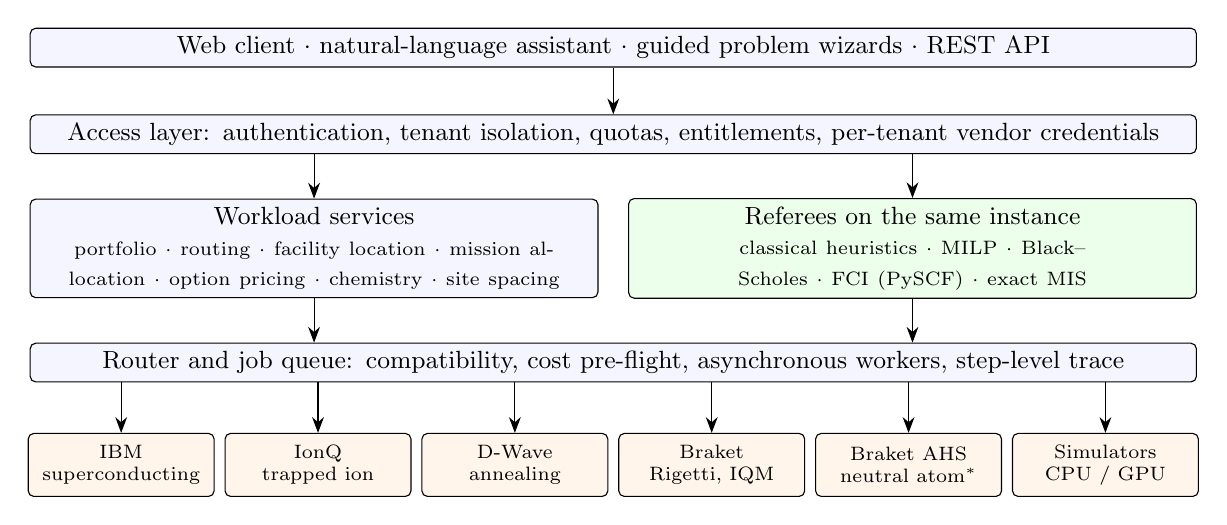
\begin{tikzpicture}[
  base/.style={draw, rounded corners=2pt, align=center, inner sep=3pt},
  box/.style={base, font=\small, fill=blue!4},
  ref/.style={base, font=\small, fill=green!8},
  hw/.style={base, font=\scriptsize, fill=orange!8, text width=2.15cm, minimum height=8mm},
  >={Stealth[length=2mm]}]
  \node[box, text width=14.6cm] (ui) at (0,0) {Web client $\cdot$ natural-language assistant $\cdot$ guided problem wizards $\cdot$ REST API};
  \node[box, text width=14.6cm] (api) at (0,-1.1) {Access layer: authentication, tenant isolation, quotas, entitlements, per-tenant vendor credentials};
  \node[box, text width=7.0cm] (wl) at (-3.8,-2.55) {Workload services\\\scriptsize portfolio $\cdot$ routing $\cdot$ facility location $\cdot$ mission allocation $\cdot$ option pricing $\cdot$ chemistry $\cdot$ site spacing};
  \node[ref, text width=7.0cm] (rf) at (3.8,-2.55) {Referees on the same instance\\\scriptsize classical heuristics $\cdot$ MILP $\cdot$ Black--Scholes $\cdot$ FCI (PySCF) $\cdot$ exact MIS};
  \node[box, text width=14.6cm] (rt) at (0,-4.0) {Router and job queue: compatibility, cost pre-flight, asynchronous workers, step-level trace};
  \foreach \x/\name/\txt in {-6.25/h1/{IBM\\superconducting}, -3.75/h2/{IonQ\\trapped ion}, -1.25/h3/{D-Wave\\annealing}, 1.25/h4/{Braket\\Rigetti, IQM}, 3.75/h5/{Braket AHS\\neutral atom$^\ast$}, 6.25/h6/{Simulators\\CPU / GPU}}
    \node[hw] (\name) at (\x,-5.3) {\txt};
  \draw[->] (ui) -- (api);
  \draw[->] (api.south -| wl.north) -- (wl.north);
  \draw[->] (api.south -| rf.north) -- (rf.north);
  \draw[->] (wl.south) -- (wl.south |- rt.north);
  \draw[->] (rf.south) -- (rf.south |- rt.north);
  \foreach \name in {h1,h2,h3,h4,h5,h6}
    \draw[->] (rt.south -| \name.north) -- (\name.north);
\end{tikzpicture}
\caption{Platform layers. Every workload service computes its referee on the
same instance it sends to the router; results are stored and displayed as a
pair. $^\ast$Local analog simulator; hardware submission in progress.}
\label{fig:architecture}
\end{figure}

\subsection{Layers}

Figure~\ref{fig:architecture} shows the layers. Users reach the platform
through a web client, a natural-language assistant that maps requests to runs
(Section~\ref{sec:assistant}), guided problem wizards, or a REST API. An
access layer authenticates the caller, separates tenants and checks quotas
and feature entitlements. It is implemented in the API of the workload
services; a gateway written in a second language, through which portfolio
runs and market data pass, repeats authentication and tenant separation.
Workload services own problem models, encodings and referees. A
router checks method--platform compatibility and estimated cost, and dispatches
long runs to asynchronous workers through a message queue. Results, traces and
audit records live in a relational database. Table~\ref{tab:codebase} gives the
size of the implementation.

\begin{table}[H]
\centering\small
\begin{tabular}{lp{7.0cm}}
\toprule
Component & Size \\
\midrule
Python services (workloads, routing, adapters, API) & 88\,k lines, 232 modules \\
Python tests & 46\,k lines, 168 files, 3\,010 passing tests \\
Gateway (Java/Spring) & 10\,k lines \\
Web client (React, including style sheets) & 62\,k lines \\
Database schema migrations & 41 \\
Vendor adapters & IBM, IonQ, D-Wave, Google Cirq, Rigetti/IQM (Braket), QCI CUDA-Q \\
Version history & more than 2\,000 commits since September 2025 \\
\bottomrule
\end{tabular}
\caption{Implementation size at the time of writing.}
\label{tab:codebase}
\end{table}

\subsection{Request lifecycle}
\label{sec:lifecycle}

A run proceeds through named steps, each recorded with metrics and a
plain-language explanation authored next to the code that produces the
numbers:
\begin{enumerate}
  \item \emph{Capture.} A wizard, the assistant or the API produces a typed
        problem instance (assets and constraints, stops and vehicles, sites
        and demand, support assets and tasks, option contract, molecule and
        bond length, candidate sites and spacing).
  \item \emph{Gate.} Entitlements, quotas and, for hardware, a vendor
        credential and cost estimate are checked before anything is queued,
        so failures surface as actionable errors rather than orphaned jobs.
  \item \emph{Encode.} The workload service builds the quantum formulation and
        records its size (variables, qubits, terms) and any approximation.
  \item \emph{Execute.} The router dispatches to a simulator or vendor
        back-end; vendor job identifiers are kept for deep links.
  \item \emph{Decode and refine.} Raw measurements are decoded; classical
        refinement, if any, runs as a separate, separately reported step.
  \item \emph{Referee.} The referee is computed on the same instance and the
        gap, error or approximation ratio is stored next to the result.
\end{enumerate}

\subsection{Credentials across process boundaries}

Tenants may bring their own vendor keys. Keys are encrypted at rest and
injected into vendor SDK calls only for the duration of a submission, through
a context variable. Context variables do not cross the boundary from the API
process to the worker process, so a credential resolved at submission is not
available where the run executes. Workers therefore resolve credentials
again and fail a hardware run for which none resolves. They do not fall back
to a simulator: a run would then be recorded under a vendor it never
reached, and a fallback that is only logged has the same effect. Hybrid
systems routinely split submission and execution across processes, so the
point is general.

\subsection{Contract drift between components}

The web client, the gateway and the workload services are written in
different languages and agree on the fields of a request by convention only.
A field sent by one component can be dropped silently by the next: a schema
library ignores undeclared keys by default, and a field that the sender
nests is not seen by a receiver that declares it at the top level. A check
that depends on such a field then does not run, and nothing fails. A
multi-language service therefore needs end-to-end contract tests; paired
requests that differ in one field are a cheap form of them.

\subsection{Natural-language assistant}
\label{sec:assistant}

The assistant translates requests (``price an at-the-money call with
amplitude estimation'', ``what is the principle of molecular energy
simulation?'') into explanations and run proposals. A rule-based layer handles
known intents and typos; a language model answers open questions using a
prompt grounded in what each workload actually does. Every answer about a
workload offers a classical and a quantum run of the same instance. Even with
explicit instructions, a language model repeatedly describes quantum methods as
``exploring all combinations at once'' or ``finding solutions faster''. A
sentence-level post-filter removes such claims except for amplitude
estimation, the only workload with a proven asymptotic query advantage.
The filter covers the free-text answers of this assistant. The advisors
inside the workload views and an automated reviewer of results are
instructed by their prompts only
(Section~\ref{sec:limitations}).
Language interfaces to quantum software therefore need an explicit
honesty layer, not only a prompt.

\subsection{Operations}

The services run on Kubernetes with GitOps delivery. Continuous integration
builds the image of a service only after its test suite has passed and, for
the back-end services, after a scan of the Python code, its dependencies and
the repository for committed secrets; an end-to-end test runs against the
deployed services afterwards. Development, staging and production are
separate clusters.

%======================================================================
\section{Correctness methodology}
\label{sec:correctness}

\inbrief{The optimisation paths take their Ising Hamiltonian from one
module, and tests compare it with the QUBO on every bitstring of reference
instances. Such a lock catches errors of sign, scale and bit order, which
return valid-looking answers without crashing. It cannot see an error that
leaves the Hamiltonian correct, so further checks guard the experiments: an
estimator is compared with its information bound, the cost Hamiltonian of
QAOA is normalised, a control is tuned on held-out instances, and a referee
that is named is also run. A test keeps the inventory of the modules that
must be behind the lock.}

\subsection{An exhaustive lock on the encoding}

The optimisation paths that need an Ising Hamiltonian take it from one
module, which converts a
quadratic unconstrained binary objective
$f(x) = \sum_i q_i x_i + \sum_{i<j} Q_{ij} x_i x_j + c$ to an Ising
Hamiltonian via $x_i = (1 - z_i)/2$:
\begin{equation}
H(z) = \sum_i h_i z_i + \sum_{i<j} J_{ij} z_i z_j + c', \qquad
h_i = -\tfrac{q_i}{2} - \tfrac{1}{4}\sum_{j\neq i} Q_{ij}, \qquad
J_{ij} = \tfrac{Q_{ij}}{4},
\end{equation}
with $c' = c + \tfrac{1}{2}\sum_i q_i + \tfrac{1}{4}\sum_{i<j} Q_{ij}$.
One path, CVaR-VQE, keeps the implementation that this module was modelled
on. Both are under the same lock: for each such path a test enumerates all
$2^n$ bitstrings of reference instances and asserts that $f(x)$ and
$H(z(x))$ agree up to rounding (on two paths up to an additive constant),
and for several paths that the constraints hold at the minimum. Paths that
hand a binary model to a vendor's annealing library convert nothing
themselves; for routing and facility location the same enumeration holds
that model to the QUBO, for the portfolio annealing methods nothing does yet
(Section~\ref{sec:limitations}). For mission allocation an enumeration
holds the QUBO to the model: on 30 instances of 6 to 14 variables every
minimiser of the QUBO satisfies the two rules it encodes and has the energy
of the exact optimum without the duty limit.

Table~\ref{tab:defects} lists the classes of error that the lock and the
checks around it catch in independently written conversions. None of them
crashes.

\begin{table}[H]
\centering\small
\begin{tabular}{p{4.2cm}p{5.0cm}p{4.6cm}}
\toprule
Error & Visible symptom & Detected by \\
\midrule
Sign flip of the linear field & Returns the complement of the intended selection ($n-K$ assets instead of $K$) & Exhaustive $f(x)=H(z)$ check \\
Pair coefficients at half weight & Plausible selections, wrong ranking of near-optimal solutions & Exhaustive check \\
QUBO coefficients on Pauli terms without conversion & Optimises a different problem; selections look reasonable & Exhaustive check \\
Big-endian strings decoded as little-endian & Correct objective value, wrong assets reported & Cross-path agreement on identical instances \\
Variance diagonal dropped & Risk term ignored for single assets & Exhaustive check \\
Equality where inequality intended (cardinality) & Opens a superfluous facility at extra cost & Brute-force optimum comparison \\
Oversized penalty weights & Feasible but mediocre solutions; annealer temperature scale dominated by penalties & Gap to referee \\
\bottomrule
\end{tabular}
\caption{Classes of error caught by the exhaustive lock and the checks
around it. Each produces a valid-looking answer.}
\label{tab:defects}
\end{table}

The same discipline extends beyond Hamiltonians. Option pricing reports the
discretisation bias separately from the statistical error and warns when the
bias dominates. Chemistry reports the error above FCI, not an absolute energy.

\subsection{What the lock cannot see}
\label{sec:audit}

An encoding test cannot detect an error that leaves the Hamiltonian correct.
Four checks on the experiments cover such cases (Table~\ref{tab:audit});
each is a referee for the experiment, not for the code (principle P8).

\begin{table}[H]
\centering\small
\begin{tabular}{p{3.3cm}p{5.2cm}p{5.3cm}}
\toprule
Error & What it produces & Check \\
\midrule
One random stream shared by all circuits of a batch & An estimator error below its Cram\'er--Rao bound and a convergence slope steeper than theory allows & The estimator is compared with its information bound; a test asserts that identical circuits in one batch return uncorrelated counts \\
Cost Hamiltonian in problem units & QAOA training that is a random search; deeper circuits no better & The Hamiltonian is divided by its largest coefficient; the exact landscape is inspected on a grid \\
Control with a fixed, untuned parameter & A gain that belongs to the tuning and not to the method & The control is tuned on held-out instances \\
Classical referee named but not run & A sampler that ``beats classical selection'' & The referee is run at matched resources \\
\bottomrule
\end{tabular}
\caption{Errors that pass an exhaustive encoding test, and the checks on the
experiments that catch them.}
\label{tab:audit}
\end{table}

\paragraph{Independent shot noise.} MLAE submits all Grover powers as one
batch, and its likelihood multiplies their probabilities as independent.
Qiskit's \texttt{StatevectorSampler}, given one seed for a batch, draws
every circuit's shots from the same random stream: two identical circuits
in one batch return identical counts, and an estimator then sees far less
noise than it assumes. The platform gives each circuit its own generator,
and regression tests assert that identical circuits in one batch are
uncorrelated. The experiments compare the estimator's error with the
Cram\'er--Rao bound at the true amplitude, which no unbiased estimator can
beat (Section~\ref{sec:res-mc}).

\paragraph{Scale of the cost Hamiltonian.} QAOA applies
$e^{-i\gamma H}$. With $H$ in problem units, facility-location penalties make
its largest Ising coefficient $8.97\times10^{4}$, while $\gamma$ starts in
$[0,\pi]$ and an optimiser's first steps are of order one: a single step
spans about $10^{5}$ periods of the dominant phase. The need to rescale
$\gamma$ for weighted problems is known~\cite{shaydulin2023,sureshbabu2024}.
The exact encoding test is blind to it, because a
correct Hamiltonian multiplied by any constant is still correct. The platform
divides the Hamiltonian by its largest coefficient
(Section~\ref{sec:res-qaoa}).

\paragraph{Controls and referees.} A control has free parameters of its own
and is tuned on instances the comparison does not use
(Section~\ref{sec:res-mis}). A classical referee that is named is also run,
at matched resources (Section~\ref{sec:res-chem}).

\paragraph{Statistics.} Confidence intervals use Student's $t$ for the
number of independent units they rest on; runs on the same instance are not
counted as independent; every point of a convergence curve has its own
seeds; every simulator is seeded; and statements about hardware are tests on
the stored counts (Section~\ref{sec:method}).

\paragraph{An inventory of what must be behind the lock.} A lock protects
what it covers. A test lists every module that builds or evaluates an Ising
Hamiltonian together with the test that locks it, and fails when such a
module is missing from the list. The test recognises a conversion by its
names; one written in plain arithmetic
under another name would pass it, and only controls on the results would
find it.

%======================================================================
\section{Workloads and encodings}
\label{sec:workloads}

\inbrief{Seven workloads, each with its quantum formulation, the methods the
platform runs on it and its referee. Three points matter for the results.
The four portfolio methods each build a variant of the intended
objective. Two encodings leave a constraint to classical repair: capacity in
facility location and the duty limit in mission allocation. And the Rydberg
mapping uses the static blockade radius, with a mapping by the dynamic
radius as its control.}

Table~\ref{tab:workloads} summarises the workloads.

\begin{table}[H]
\centering\small
\begin{tabular}{p{2.4cm}p{3.1cm}p{3.6cm}p{3.6cm}}
\toprule
Workload & Quantum formulation & Quantum methods & Referee \\
\midrule
Portfolio selection & QUBO, $n$ variables & QAOA, CVaR-VQE, PCE, BF-DCQO, annealing & Enumeration of the QUBO (exact, this paper); max-Sharpe weights (a different problem) \\
Vehicle routing & Assignment QUBO, $n_{\mathrm{stops}}\times n_{\mathrm{clusters}}$ & Annealing, QAOA & Savings construction (heuristic) \\
Facility location & QUBO, $n_s + n_s n_d$ + slack & Annealing, QAOA & Greedy + local search (heuristic); MILP (exact) \\
Option pricing & $n$-qubit price register + ancilla & MLAE & Black--Scholes (exact) \\
Ground-state energy & $2\,n_{\mathrm{orb}}$ qubits & SqDRIFT + SQD & FCI (exact); selected CI (this paper) \\
Spaced site selection & One atom per site & Adiabatic Rydberg sweep & Exact MIS (exact) \\
Mission resource allocation & QUBO, one variable per allowed asset--task pair & Simulated annealing (classical) & MILP (exact); greedy fill (heuristic) \\
\bottomrule
\end{tabular}
\caption{Workloads, formulations and referees.}
\label{tab:workloads}
\end{table}

\paragraph{Portfolio selection.} Mean--variance~\cite{markowitz1952} over
binary selection with a cardinality penalty,
$\min_x \gamma\, x^\top \Sigma x - \mu^\top x + \lambda (\mathbf 1^\top x - K)^2$,
with shrinkage covariance~\cite{ledoit2004}. This is the intended
formulation. The four gate-model methods each build a variant of it
(Table~\ref{tab:pf-corrected}); they differ in the weight of the risk term
and in whether a cardinality term is present. The classical baseline returns
continuous maximum-Sharpe weights, which is a different problem from all of
them; the exact referee used in this paper is an enumeration of each
method's own QUBO.

\paragraph{Vehicle routing.} A capacitated, time-windowed routing problem is
decomposed into a stop-to-vehicle assignment QUBO with pairwise distance terms
followed by classical sequencing. The referee is a savings
construction~\cite{clarke1964}.

\paragraph{Capacitated facility location (CFLP).} Opening variables $y_j$ and
assignment variables $x_{ij}$, objective
$\sum_j f_j y_j + \sum_{i,j} c_{ij} x_{ij}$~\cite{owen1998}, one-hot service
constraints, linking terms $x_{ij}(1 - y_j)$, and an upper bound on open sites
encoded with slack bits whose weights represent $[0, m]$ exactly.
\emph{Capacity is not in the QUBO}; it is enforced by classical repair. The
QUBO therefore encodes the uncapacitated problem, and its ground state need
not be a feasible plan (Section~\ref{sec:res-cflp}). Annealing samples propose
an open set; the same drop/swap local search used by the heuristic referee
refines it. For QAOA the Ising Hamiltonian is divided by its largest
coefficient.

\paragraph{European option pricing.} A log-normal terminal price is
discretised onto $2^n$ bins and loaded by a tree of uniformly controlled
rotations; one more uniformly controlled rotation encodes the payoff into an
ancilla amplitude $a$. MLAE~\cite{suzuki2020} runs the state preparation
$\mathcal A$ followed by $k$ Grover iterates for $k = 0, 1, 2, 4, \dots, m$
with a fixed number of shots per power, and fits $a$ by maximum likelihood.

\paragraph{Molecular ground-state energy.} For H$_2$, LiH, H$_2$O and N$_2$
(STO-3G), the SqDRIFT procedure~\cite{sqdrift2025} samples configurations from
randomized qDRIFT evolutions~\cite{campbell2019} of the Hartree--Fock state
and diagonalizes the Hamiltonian in the subspace spanned by the sampled
configurations with configuration recovery~\cite{kanno2023,robledo2024}.

\paragraph{Spaced site selection on Rydberg arrays.} Choose as many candidate
sites as possible with no two chosen sites closer than $s$: maximum independent
set (MIS) on the unit-disk conflict graph. Atoms at scaled site coordinates
evolve under
\begin{equation}
H(t) = \sum_i \frac{\Omega(t)}{2}\,\sigma^x_i - \Delta(t)\sum_i n_i
      + \sum_{i<j} \frac{C_6}{|\mathbf r_i - \mathbf r_j|^6}\, n_i n_j,
\end{equation}
with $\Omega$ ramped up and down while $\Delta$ sweeps from negative to
positive~\cite{pichler2018,ebadi2022}. At the end of the sweep $\Omega = 0$
and the Hamiltonian is diagonal: adding atom $j$ to an excited set $S$ changes
the energy by $-\Delta_{\mathrm{end}} + \sum_{i\in S} V_{ij}$, so pairs with
$V_{ij} > \Delta_{\mathrm{end}}$ are excluded. The relevant length is the
\emph{static blockade radius} of the final detuning~\cite{wurtz2023},
\begin{equation}
r_c = \left(C_6/\Delta_{\mathrm{end}}\right)^{1/6},
\end{equation}
not the \emph{dynamic} radius $R_b = (C_6/\Omega)^{1/6}$ of the drive. A
mapping that scales coordinates to $R_b$ and sweeps to
$\Delta_{\mathrm{end}} = 6\,\Omega$ leaves conflicting pairs between
$0.74\,R_b$ and $R_b$ unblockaded at readout; it is the control of
Section~\ref{sec:res-mis}. The platform scales the
spacing threshold to $r_c$, chooses $\Omega_{\max} = \Delta_{\mathrm{end}}/2$,
and places the threshold at the geometric mean of the longest conflicting and
shortest non-conflicting distance. This is established device
practice~\cite{wurtz2023}, not a new mapping; Section~\ref{sec:res-mis}
measures what the mismatch cost. The minimum atom spacing
$d_{\min} = 4\,\mu$m and a design floor on the final detuning,
$\Delta_{\mathrm{end}}^{\min} = 2.5$\,Mrad/s (below it $\Omega_{\max}$ times
the $4\,\mu$s sweep falls under 5\,rad), bound the ratio of the mapped
threshold $t$ to the closest pair of sites:
\begin{equation}
\frac{t}{d_{\mathrm{closest}}} \;\le\; \frac{r_c^{\max}}{d_{\min}}
\;=\; \frac{(C_6/\Delta_{\mathrm{end}}^{\min})^{1/6}}{4\,\mu\mathrm{m}}
\;\approx\; 2.85
\end{equation}
for $C_6 = 5.42\times 10^{-24}$\,rad\,m$^6$/s. Instances beyond this ratio are
refused rather than embedded unfaithfully.

\paragraph{Mission resource allocation.} Support and logistics allocation:
assets (helicopters, vehicles, teams) with capabilities, a base, an
availability window and a duty limit take tasks that each need one
capability at a fixed place and time and carry a priority. The workload does
not model the use of force: there are no targets and no effects on an
adversary. An asset--task pair is \emph{allowed} when the asset has the
capability, can reach the task from its base and be back inside its window
(straight-line travel), the task alone fits the duty limit, and the weight
$w_{at} = 1000\,p_t - c_{at}$ is positive, with $p_t$ the priority and
$c_{at}$ the cost of the task hours and of a round trip from the base. The
model maximises $\sum w_{at} x_{at}$ over the allowed pairs subject to three
rules: a task is served at most once; an asset does not take two tasks it
cannot travel between in time; the task hours of an asset stay within its
duty limit. The QUBO has one binary per allowed pair and penalises
violations of the first two rules with $1.05$ times the largest weight.
\emph{The duty limit is not in the QUBO.} Every sample is repaired (pairs
are dropped until no rule is violated) and filled (unassigned tasks are
added greedily, by priority, where they fit); the greedy baseline of the
workload is this fill applied to an empty plan. The referee is the exact
mixed-integer model.

%======================================================================
\section{Experimental methodology}
\label{sec:method}

\inbrief{All experiments call the platform's own modules and are seeded.
Means carry 95\% intervals over independent runs or instances, with the unit
of analysis stated. Each result is paired with the strongest referee and
control we could compute at its size. Eight hardware rounds ran on three IBM
Heron processors; from the second round on the analysis was fixed before the
first job, and the one probe designed after a result is labelled post hoc.}

\paragraph{Setup.} All experiments call the platform's own modules; no
separate research code reimplements the methods. They ran on a single
workstation (AMD Ryzen 9 5950X, 16 cores, 64\,GB RAM) with Qiskit 2.5.2,
Qiskit Aer 0.17, \texttt{qiskit-addon-sqd}~0.13, PySCF~2.14~\cite{pyscf2020},
Amazon Braket SDK 1.117 (local analog simulator), D-Wave Ocean
(\texttt{neal}), SciPy~1.17 with HiGHS~\cite{virtanen2020,huangfu2018}. Unless
stated otherwise, quantum circuits were sampled from exact state vectors
without noise (``noiseless simulation''); the analog protocol used the Braket
local solver of the ideal Rydberg Hamiltonian. Runs are seeded, and every
script except the first Rydberg one (E3) pins numerical libraries to one
thread per process; repeated runs of E1, E11 and E12 were bit-identical. The
portfolio methods take a seed; E21, E23, E24
and E25 pass it through the product's own argument.

\paragraph{Cost units.} For amplitude estimation, one \emph{oracle query} is one
application of the state-preparation unitary $\mathcal A$; a shot at Grover
power $k$ costs $2k+1$ queries. For classical Monte Carlo, the cost unit is one
payoff evaluation; with antithetic variates~\cite{glasserman2003}, $N$
evaluations form $N/2$ independent pairs.

\paragraph{Statistics.} Means are reported with two-sided 95\% Student-$t$
intervals over independent runs or instances, with the unit of analysis
stated; at least five seeds are used per setting. Root-mean-square errors
carry bootstrap percentile intervals~\cite{efron1979} over 50 independent
replicates. Proportions carry Wilson~\cite{wilson1927} or exact
Clopper--Pearson~\cite{clopper1934} intervals and are tested with exact
binomial or Fisher tests. Paired designs are tested with the Wilcoxon
signed-rank test~\cite{wilcoxon1945}, unpaired ones with the Mann--Whitney
$U$ test; where a sample takes only a few distinct values a sign test is
given next to the $t$-test. Every (method, point, replicate) cell has its own seed derived from
a seed sequence, so points on a curve are independent. $p$-values are
reported unadjusted; where several tests bear on one claim we say how many.

\paragraph{Referees and controls.} Each result is paired with the strongest
check we could compute at its size: the Cram\'er--Rao bound and classical
sampling of the same discretised distribution for amplitude estimation; a
proven MILP optimum for facility location, for the capacitated problem and
for the uncapacitated problem the QUBO encodes; exact evaluation of all
$2^{18}$ amplitudes with closed-form uniform references for QAOA; for
portfolio selection, enumeration of each method's own QUBO, uniform bits
pushed through the same production code, a reordering of the input
columns and, for what the product displays, the selection replaced by
every asset; random
strings, an FCI-informed oracle and a selected-CI curve, all scored by one
solver, for sample-based diagonalization; a control tuned on held-out
instances for the Rydberg mapping; for mission resource allocation, a
proven MILP optimum, the greedy baseline, uniform bitstrings through the
production repair and fill, in equal number and in equal time, and, for a
gate-based sampler, all $2^n$
bitstrings through the same two stages; and, on hardware, depth-matched null
circuits, a readout calibration in the same job, and device samples shuffled
within each qubit's marginal.

\paragraph{Hardware protocol.} Hardware runs used \texttt{ibm\_marrakesh};
round~4 ran on \texttt{ibm\_kingston} and round~6 on \texttt{ibm\_fez}. All
three are 156-qubit IBM Heron~r2 processors, used
through IBM Quantum (Open plan), with the
platform's settings: transpilation at optimisation level~3 (best of eight
seeds by two-qubit gate count in rounds~2 to~5; one pass, as the product
makes it, in rounds~6 and~7; in round~8 best of eight seeds without error
data, and the qubits chosen as Section~\ref{sec:res-hw8} describes), SamplerV2 with XY4 dynamical
decoupling~\cite{viola1999} and Pauli twirling of two-qubit
gates~\cite{wallman2016}, and no further error mitigation, with one
exception: the Estimator jobs of round~6 set the same two options, and the
service added its defaults for an Estimator, measurement twirling and
readout mitigation of the expectation values. Round~1 (ten
jobs, 41\,s) ran the platform's production path end to end. Round~2 (five
jobs, 124\,s) added matched nulls and controls. Its analysis plan ---
hypotheses, test statistics, shot counts, the rule that no run is excluded
--- was fixed in writing before the first job was submitted. One follow-up
experiment (the screened-qubit probe of Section~\ref{sec:res-hw}) was
designed after a round-2 result was seen; it is labelled post hoc wherever
it appears. Its plan was written down before the probe was submitted and
amended once, after a failed transpilation and before any probe circuit had
run. Round~3 (six jobs, 400\,s) sampled portfolio circuits whose angles had
been trained on the simulator. Its design was fixed before the first job
and amended once before any device data existed
(Section~\ref{sec:res-hw3}). Round~4 (one job, 37\,s) repeated the first
experiment of round~2 on the second device; its plan, with the rule that
chose the device, was committed before the job
(Section~\ref{sec:res-hw4}). Round~5 (two jobs, 156\,s) tested amplitude
estimation against ideal sampling at equal queries on screened qubits of
the first device, with its criterion committed before the first job
(Section~\ref{sec:res-hw5}). Round~6 (20 jobs, 310\,s) ran the product's
own hardware path for portfolio QAOA, which trains on the device, on the
device that path chose; its plan was committed before the first job and
amended once before any training job (Section~\ref{sec:res-hw6}). Round~7
(three jobs, 37\,s) put the product's SqDRIFT circuits for a 24-qubit
active space on the first device, with its plan committed before the first
job (Section~\ref{sec:res-hw7}). Round~8 (one job, 48\,s) ran one circuit
on the first device on the qubits chosen from calibration data of three
ages; its plan was committed before the first snapshot of those data and
amended once before any job (Section~\ref{sec:res-hw8}). Every job
identifier and the raw counts of
rounds~2 to~8 are in the result files. The published calibration,
which the transpiler uses to place circuits, was not recent: its readout
data were 3.9~days old when round~2 ran, and the record of the second
device was dated 44~hours before the job of round~4.

\paragraph{Reproducibility.} Experiment scripts, raw JSON results and figure
generators are versioned with the paper source. Each result file records the
code commit and library versions.

%======================================================================
\section{Results}
\label{sec:results}

\inbrief{The experiments are reported by workload: option pricing
(Section~\ref{sec:res-mc}), molecular energy (\ref{sec:res-chem}), facility
location and the QAOA on its QUBO (\ref{sec:res-cflp},
\ref{sec:res-qaoa}), portfolio selection
(\ref{sec:res-portfolio2}), vehicle routing
(\ref{sec:res-fleet}), site selection on Rydberg arrays
(\ref{sec:res-mis}), mission resource allocation (\ref{sec:res-mission})
and eight rounds on hardware (\ref{sec:res-hw}). Each subsection opens with
what was run and what came out, and closes with its finding. Apart from the
hardware rounds, the quantum results come from noiseless simulators and the
annealing results from simulated annealing.}

\subsection{Option pricing: a measured gain, on its information bound}
\label{sec:res-mc}

\inbrief{Does maximum-likelihood amplitude estimation (MLAE) deliver its
proven query advantage, and at what circuit depth? One at-the-money European
call on five price qubits, 50 replicates per point, against classical
sampling of the same 32-bin grid and against antithetic sampling of the
continuous distribution. The error of MLAE falls with slope $-0.96$ where
both classical samplers show the theoretical $-1/2$, and it is $0.83$ to
$1.16$ times its Cram\'er--Rao bound. At a root-mean-square error of $0.01$
MLAE needs $38\times$ fewer queries than sampling of the same grid and
$17\times$ fewer than antithetic sampling of the continuous distribution.
The circuits that deliver this have thousands of two-qubit gates:
$13\,374$ at Grover power 64.}

Instance: at-the-money European call, $S_0 = K = 100$, $r = 0.05$,
$\sigma = 0.2$, $T = 1$; Black--Scholes~\cite{blackscholes1973} price
$10.4506$; $n = 5$ price qubits (discretised target $10.4376$, amplitude
$a = 0.0640$). MLAE with 100 shots per Grover power and largest powers
$m = 1\dots256$; classical Monte Carlo with antithetic variates on the
continuous log-normal, $10^2$--$10^7$ evaluations, scored against
Black--Scholes; and, as a like-for-like control, plain classical sampling of
the same 32-bin distribution that MLAE encodes, scored against the same
discretised target. Every point has 50 independent replicates.

\begin{figure}[H]
\centering
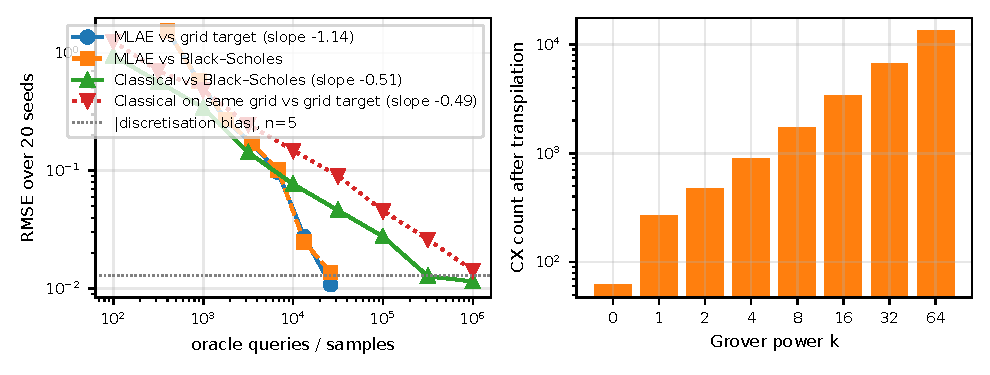
\includegraphics[width=\linewidth]{figures/mlae_convergence.pdf}
\caption{Left: RMSE over 50 replicates against oracle queries (MLAE) or payoff
evaluations (classical), with bootstrap 95\% bands. MLAE is scored against its
discretised target and shown with its Cram\'er--Rao bound; classical sampling
is shown on the same 32-bin grid and, with antithetic variates, on the
continuous distribution against Black--Scholes; the dotted line is the
discretisation bias at $n=5$. Right: MLAE RMSE divided by the Cram\'er--Rao
bound at the true amplitude, per schedule.}
\label{fig:mlae}
\end{figure}

\begin{table}[H]
\centering\footnotesize\setlength{\tabcolsep}{4pt}
\begin{tabular}{rrlrrcrl}
\toprule
$m$ & Queries & RMSE [95\% CI] & Bound & Ratio & Coverage & CX (deepest) & $P_{\mathrm{ok}}$ at $10^{-3}$ \\
\midrule
1 & 400 & 1.325 [1.05, 1.59] & 1.262 & 1.05 & 45/50 & 270 & 0.76 \\
2 & 900 & 0.642 [0.52, 0.75] & 0.675 & 0.95 & 49/50 & 478 & 0.62 \\
4 & 1\,800 & 0.319 [0.25, 0.38] & 0.371 & 0.86 & 49/50 & 894 & 0.41 \\
8 & 3\,500 & 0.204 [0.17, 0.23] & 0.198 & 1.03 & 48/50 & 1\,726 & 0.18 \\
16 & 6\,800 & 0.120 [0.095, 0.142] & 0.103 & 1.16 & 45/50 & 3\,390 & 0.034 \\
32 & 13\,300 & 0.053 [0.041, 0.065] & 0.053 & 1.00 & 46/50 & 6\,718 & 0.0012 \\
64 & 26\,200 & 0.022 [0.018, 0.026] & 0.027 & 0.83 & 50/50 & 13\,374 & $1.6\times10^{-6}$ \\
128 & 51\,900 & 0.0117 [0.0095, 0.0138] & 0.0134 & 0.87 & 49/50 & 26\,686$^\dagger$ & $<10^{-11}$ \\
256 & 103\,200 & 0.0077 [0.0065, 0.0089] & 0.0067 & 1.14 & 45/50 & 53\,310$^\dagger$ & $<10^{-23}$ \\
\bottomrule
\end{tabular}
\caption{MLAE on a noiseless simulator, 50 replicates per row. RMSE against
the discretised target with a bootstrap interval; the Cram\'er--Rao bound at
the true amplitude and the ratio of the two; the number of replicates whose
own 95\% interval (from the Fisher standard error) contains the target; the CX
count of the deepest circuit after transpilation to
$\{\mathrm{CX}, R_z, \sqrt{X}, X\}$ with all-to-all connectivity; and
$P_{\mathrm{ok}} = (1-\varepsilon)^{N_{\mathrm{CX}}}$, the probability that no
two-qubit gate of that circuit fails at error rate $\varepsilon$.
$^\dagger$From $N_{\mathrm{CX}} = 62 + 208\,k$, which holds exactly for the
transpiled circuits at $k \le 64$.}
\label{tab:mlae}
\end{table}

The fitted error slope is $-0.957$ (95\% CI $[-0.990, -0.922]$) for MLAE over
all schedules and $-0.984$ $[-1.032, -0.933]$ for $m \ge 4$; $-0.495$
$[-0.510, -0.479]$ for antithetic sampling of the continuous distribution;
and $-0.495$ $[-0.512, -0.477]$ for plain sampling of the same 32-bin grid
(Figure~\ref{fig:mlae}). The classical slopes match the theoretical $-1/2$.
The MLAE slope matches that of its own Cram\'er--Rao bound over the same
schedules ($-0.956$, and $-0.993$ for $m \ge 4$; the bound reaches $-1$ only
asymptotically). The estimator is
efficient: the ratio of RMSE to the bound lies between 0.83 and 1.16, and
its bootstrap interval contains 1 at eight of nine schedules
(Table~\ref{tab:mlae}). Its reported uncertainty is calibrated: the
estimator's own 95\% interval contains the target in 426 of 450 runs
(94.7\%).

Read inside the measured range of both methods by log--log interpolation,
RMSE $0.01$ against the discretised target takes $6.7\times10^{4}$ MLAE
queries, $2.6\times10^{6}$ plain samples of the same grid and
$1.1\times10^{6}$ antithetic evaluations of the continuous distribution: a
ratio of $38\times$ like for like, of which a standard classical
variance-reduction technique recovers more than half ($17\times$). At RMSE
$0.03$ the ratios are $11\times$ and $5.9\times$; at $0.1$ they are
$2.5\times$ and $1.2\times$.

Three further observations matter for practice.
\begin{enumerate}
  \item \emph{Bias dominates at small $n$.} The discretisation bias is
        $+5.42$, $+1.11$, $+0.21$, $-0.013$, $+0.018$ at $n = 2\dots6$. Below
        $n = 5$ no number of shots brings MLAE within $0.1$ of the true price,
        and at $n = 5$ its error against Black--Scholes stops falling at the
        bias ($0.017$ and $0.014$ at $m = 128$ and $256$). This regime would
        be invisible without an exact referee.
  \item \emph{The gain lives at depths hardware does not reach.} The circuit
        at Grover power $k$ has $62 + 208\,k$ CX gates before routing. With a
        two-qubit error rate of $10^{-3}$ the circuit at $k = 8$ runs without
        a two-qubit error with probability $0.18$ and at $k = 64$ with
        $1.6\times10^{-6}$. Schedules that fit ($m \lesssim 4$--$8$) reach
        RMSE $0.2$--$0.3$, which antithetic classical sampling matches with
        $1$--$3\times10^{3}$ evaluations. Section~\ref{sec:res-hw} measures the
        limit on a device and finds it lower than $P_{\mathrm{ok}}$ suggests.
  \item \emph{Queries are not costs.} One query here is hundreds of
        two-qubit gates; one classical evaluation is a few nanoseconds. The
        state preparation uses generic uniformly controlled rotations, whose
        cost grows as $O(2^n)$; more efficient loaders would shift the numbers
        but not the conclusion. Low-depth variants~\cite{giurgica2022} and
        error correction~\cite{beverland2022} are prerequisites for the
        asymptotic gain to matter.
\end{enumerate}

\finding{The one proven asymptotic advantage on the platform is reproducible
on a simulator, where the estimator sits on its information bound. The
crossover with classical sampling is set by circuit depth, not by query
count.}

\subsection{Molecular energy: exactness tracks coverage, and selected CI wins}
\label{sec:res-chem}

\inbrief{When sample-based diagonalization returns an exact energy, is that
the sampler's doing? SqDRIFT with SQD on H$_2$, LiH, H$_2$O and N$_2$,
noiseless, five seeds per setting, against FCI. H$_2$ and LiH are exact
because the subspace spans almost the whole configuration space. For N$_2$
the same solver was run on subspaces of the same dimension chosen
classically: the pipeline is 14--80$\times$ more accurate than random
strings and, in all 25 runs, less accurate than a classical selected CI, by
a mean factor of 6--41 per setting.}

SqDRIFT with 25, 100 or 200 circuits per evolution time, 100 shots each,
noiseless simulation, five seeds per setting. All molecules use STO-3G
without a frozen core; N$_2$ has 10 spatial orbitals and (7,7) electrons, so
its FCI dimension is $\binom{10}{7}^2 = 14{,}400$. \emph{Coverage} is the SQD
subspace dimension divided by the FCI dimension. SQD diagonalizes in the
Cartesian product of the distinct $\alpha$- and $\beta$-strings it has seen,
so a few hundred sampled configurations can span thousands of determinants.
Table~\ref{tab:chem} and Figure~\ref{fig:chem} relate the error to coverage.

\begin{table}[H]
\centering\footnotesize\setlength{\tabcolsep}{4pt}
\begin{tabular}{lrrrrlc}
\toprule
Molecule & Qubits & FCI dim. & Circuits & Coverage & $|$Error$|$ (mHa), mean $\pm$ CI (max) & $\le 1.6$\,mHa \\
\midrule
H$_2$ & 4 & 4 & 25, 100 & 100\% & 0.000 & 10/10 \\
LiH & 12 & 225 & 25 & $88 \pm 9\%$ & $0.0005 \pm 0.0014$ (0.003) & 5/5 \\
LiH & 12 & 225 & 100 & $92 \pm 9\%$ & 0.000 & 5/5 \\
H$_2$O & 14 & 441 & 25 & $53 \pm 11\%$ & $0.36 \pm 0.50$ (1.08) & 5/5 \\
H$_2$O & 14 & 441 & 100 & $75 \pm 20\%$ & $0.09 \pm 0.12$ (0.20) & 5/5 \\
N$_2$ eq. & 20 & 14\,400 & 25 & $19.0 \pm 3.7\%$ & $5.09 \pm 1.39$ (7.05) & 0/5 \\
N$_2$ eq. & 20 & 14\,400 & 100 & $40.6 \pm 6.9\%$ & $0.62 \pm 0.27$ (0.91) & 5/5 \\
N$_2$ 1.8\,\AA & 20 & 14\,400 & 25 & $19.0 \pm 7.1\%$ & $15.8 \pm 9.0$ (23.9) & 0/5 \\
N$_2$ 1.8\,\AA & 20 & 14\,400 & 100 & $43.1 \pm 2.5\%$ & $3.70 \pm 2.79$ (5.70) & 1/5 \\
N$_2$ 1.8\,\AA & 20 & 14\,400 & 200 & $45.4 \pm 4.4\%$ & $2.46 \pm 2.05$ (4.44) & 1/5 \\
\bottomrule
\end{tabular}
\caption{SqDRIFT + SQD against FCI: mean and 95\% interval over five seeds.}
\label{tab:chem}
\end{table}

\begin{figure}[H]
\centering
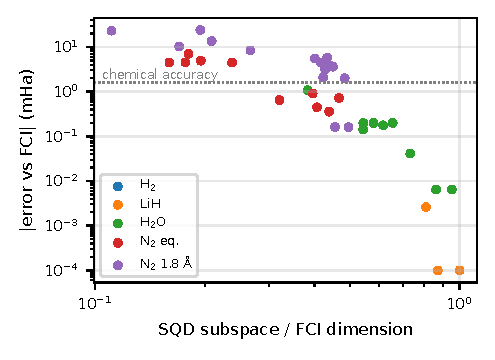
\includegraphics[width=0.5\linewidth]{figures/chemistry_subspace.pdf}
\caption{Absolute error against FCI versus subspace coverage, one point per
run. Errors below $10^{-4}$\,mHa are drawn at $10^{-4}$. The dotted line is
chemical accuracy.}
\label{fig:chem}
\end{figure}

H$_2$ and LiH are exact because the subspace spans almost the entire FCI
space: once all relevant determinants are present, diagonalization is exact
whatever the sampler produced. The first informative instance is N$_2$. At
equilibrium it reaches chemical accuracy at 41\% coverage in all five runs.
Stretched to $1.8$\,\AA, where static correlation is strong, it does so in
one run of five at 43--45\% coverage, and the spread between seeds is as
large as the mean. The sampler concentrates near the Hartree--Fock state:
only 154--553 distinct valid configurations were seen across
5\,000--40\,000 shots. With one thread per process a seed is
bit-reproducible: a second process returned the same energy to all digits,
and the two scripts that run these settings agree exactly.

\paragraph{Is the sampler better than classical selection?}
Exactness and failure alike say nothing about the sampler unless the same
diagonalization is run on classically chosen configurations of the same
size. For each N$_2$ run we scored five ways of choosing $\alpha$- and
$\beta$-strings with one solver (PySCF's fixed-space selected-CI
kernel~\cite{pyscf2020}): the platform pipeline; every string SqDRIFT
sampled, without the pipeline's subsampling and recovery; Hartree--Fock plus
uniformly random strings at the pipeline's dimension; the strings with the
largest weight in the exact FCI wave function at that dimension (an oracle:
it uses the answer); and a classical selected
CI~\cite{huron1973,holmes2016}. For the last we ran PySCF's selected-CI
solver, which grows a product of $\alpha$- and $\beta$-string sets by a
heat-bath-style criterion, over 13 selection thresholds and interpolated its
error at the pipeline's dimension, never extrapolating
(Table~\ref{tab:chemctl}, Figure~\ref{fig:sci}).

\begin{table}[H]
\centering\footnotesize\setlength{\tabcolsep}{3.5pt}
\begin{tabular}{lrrrrrrr}
\toprule
 & & \multicolumn{4}{c}{At the pipeline's dimension} & & \\
Setting & Coverage & Pipeline & Random & Selected CI & Oracle & All strings (coverage) & Pipeline / SCI \\
\midrule
N$_2$ eq., 25 & 19.0\% & $5.09 \pm 1.39$ & $87 \pm 20$ & $0.82 \pm 0.25$ & 0.30 & $1.72 \pm 0.94$ (30\%) & $6.5 \pm 2.3$ \\
N$_2$ eq., 100 & 40.6\% & $0.62 \pm 0.27$ & $49 \pm 10$ & $0.09 \pm 0.14$ & 0.006 & $0.17 \pm 0.14$ (62\%) & $19 \pm 29$ \\
N$_2$ 1.8\,\AA, 25 & 19.0\% & $15.8 \pm 9.0$ & $223 \pm 44$ & $1.24 \pm 1.37$ & 0.30 & $7.1 \pm 5.5$ (33\%) & $17 \pm 11$ \\
N$_2$ 1.8\,\AA, 100 & 43.1\% & $3.70 \pm 2.79$ & $127 \pm 24$ & $0.084 \pm 0.026$ & 0.002 & $0.12 \pm 0.10$ (62\%) & $41 \pm 31$ \\
N$_2$ 1.8\,\AA, 200 & 45.4\% & $2.46 \pm 2.05$ & $130 \pm 46$ & $0.065 \pm 0.046$ & 0.001 & $0.04 \pm 0.07$ (73\%) & $38 \pm 30$ \\
\bottomrule
\end{tabular}
\caption{Error above FCI (mHa) for N$_2$ subspaces chosen five ways, mean
$\pm$ 95\% interval over five seeds; the number after each setting is the
circuits per evolution time. ``Pipeline'' is SqDRIFT + SQD as shipped.
``All strings'' diagonalizes every sampled string at its own, larger
coverage. The last column is the mean of the per-run ratio. The strings
within two excitations of Hartree--Fock (50\% coverage) give 1.90\,mHa at
equilibrium and 15.4\,mHa at 1.8\,\AA.}
\label{tab:chemctl}
\end{table}

\begin{figure}[H]
\centering
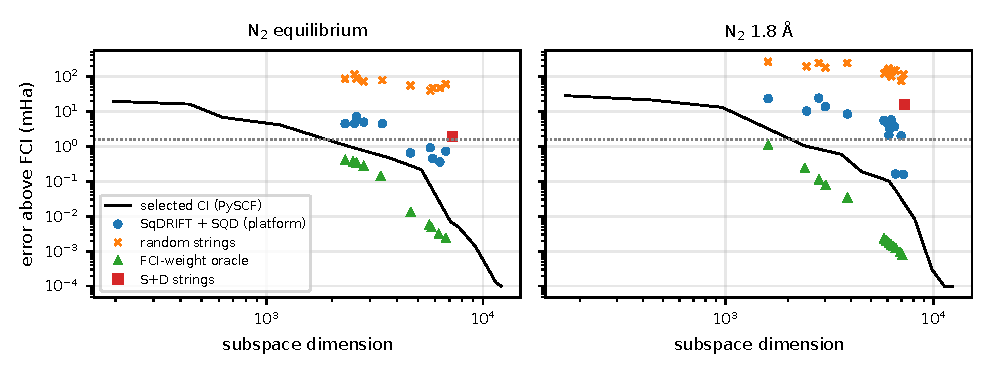
\includegraphics[width=0.9\linewidth]{figures/sqd_selected_ci.pdf}
\caption{Error above FCI against subspace dimension for N$_2$. Line: PySCF
selected CI over a sweep of selection thresholds. Points: one per SqDRIFT
run for the pipeline, for random strings and for the FCI-weight oracle at
the same dimension; the square is the singles-and-doubles string set. The
dotted line is chemical accuracy.}
\label{fig:sci}
\end{figure}

The pipeline is 14--80$\times$ more accurate than random strings at the same
dimension (ratio of the mean errors), so the sampler is not merely filling
the space. It is also less accurate than selected CI at the same dimension
in all 25 runs, by a factor of 2.3--69; the mean factor per setting is
6--41. Selected CI is within chemical accuracy at 16--17\% coverage for
both geometries (the first point of its curve beyond 8\%); the pipeline
needs 41\% at equilibrium and
does not reach it reliably for stretched N$_2$. The oracle shows how much
room is left: at 41--45\% coverage a product space of the pipeline's size
can hold the ground state to a few $\mu$Ha.

The table holds a second result. Diagonalizing every sampled string directly
is more accurate than the shipped pipeline in all 25 runs, by 2--60$\times$
in the mean error; the pipeline subsamples
300 configurations three times and applies configuration recovery. At this
size the full product space of the samples is trivially affordable; the
subsampling that makes SQD scale costs accuracy here. Selected CI at that
larger dimension is more accurate again, by a mean factor of 5--140 in the
21 of 25 runs where its error is still resolved. The selected-CI
referee is itself conservative: a determinant-based selected CI is not
confined to product spaces and would be more compact still. All of this is
noiseless.

\finding{Exact results at small sizes say nothing about the quantum sampler.
At matched subspace dimension the noiseless SqDRIFT pipeline lies between
random selection, which is 14--80$\times$ worse, and classical selected CI,
which is 6--41$\times$ better. A referee that is named must also be run.}

\subsection{Facility location: a weak referee, and a QUBO for another problem}
\label{sec:res-cflp}

\inbrief{Four seeded instances from 18 to 2\,444 QUBO variables, each with
an optimum proven by a MILP solver, both for the capacitated problem and for
the uncapacitated problem that the QUBO encodes; two simulated annealers
with 10 seeds. The platform's heuristic baseline is $2.2$--$3.4\%$ above the
optimum on the two larger instances. The optimum of the QUBO violates
capacity on every instance, so the feasibility of the pipeline comes from
its classical repair. After repair and local search, annealing is on average
no better than the heuristic that shares the local search, and worse on the
largest instance.}

Four seeded instances from 18 to 2\,444 QUBO variables. The exact optimum was
computed with HiGHS, both for the capacitated problem and for the
uncapacitated problem that the QUBO encodes; samplers ran over 10 seeds.
Table~\ref{tab:cflp}.

\begin{table}[H]
\centering\footnotesize\setlength{\tabcolsep}{3pt}
\begin{tabular}{lrrrrll}
\toprule
 & & Exact & QUBO & Heuristic & \multicolumn{2}{c}{Annealing, refined (raw feasible)} \\
Instance & Vars & (time) & optimum & referee & \texttt{neal} & NumPy \\
\midrule
2 of 4, 3 demand & 18 & 44\,522 ($<$0.01\,s) & $-19.7\%$ & $+0.00\%$ & $+0.00\%$ (0/10) & $+0.00\%$ (0/10) \\
3 of 6, 8 demand & 56 & 64\,553 (0.01\,s) & $-33.4\%$ & $+0.00\%$ & $+0.00\%$ (1/10) & $+0.00\%$ (1/10) \\
5 of 12, 20 demand & 255 & 141\,388 (3.0\,s) & $-52.2\%$ & $+3.36\%$ & $+3.94 \pm 0.67\%$ (0/10) & $+3.62 \pm 0.80\%$ (0/10) \\
8 of 40, 60 demand & 2\,444 & 290\,279 (118\,s) & $-54.0\%$ & $+2.17\%$ & $+3.50 \pm 0.91\%$ (0/10) & refused \\
\bottomrule
\end{tabular}
\caption{Facility location: cost relative to the proven optimum of the
capacitated problem. ``QUBO optimum'' is the proven optimum of the
uncapacitated problem the QUBO encodes; it violates capacity on every
instance. ``Refined'' is the gap after the shared local search (mean $\pm$
95\% interval over 10 seeds); in brackets, the seeds whose raw sample
satisfied all constraints including capacity.}
\label{tab:cflp}
\end{table}

Four conclusions follow. First, the platform's heuristic referee was itself
$2.2$--$3.4\%$ from optimal on the two larger instances; results that
``matched the baseline'' there were not near-optimal. Second, the QUBO does
not encode the problem the referee solves. Without a capacity term its
optimum overfills sites and costs 20--54\% less than the true optimum, so a
perfect sampler would return an infeasible plan on every instance. That raw
samples were feasible in at most 1 of 10 seeds is a property of the
encoding, not of the sampler: the pipeline's feasibility comes from repair by
construction. Third, annealing followed by repair was on average no better
than the heuristic referee, with which it shares the local search. The
refined results take only a few distinct values, the local optima of that
search. On the 255-variable instance 14 of the 20 runs ended above the
referee, 3 at it and 3 below it (at $+1.4\%$ and $+1.9\%$); the mean
differences are within noise ($p = 0.08$ and $0.47$, one-sample $t$-tests
against the referee's gap; sign tests $p = 0.04$ and $0.29$). On the largest
instance annealing was never better and was worse in 6 of 10 runs
($+3.50 \pm 0.91\%$ against $+2.17\%$; $t$-test $p = 0.009$, sign test
$p = 0.03$). Fourth, more annealing does not improve the refined answer. On
the 255-variable instance, ten times the reads (\texttt{neal}) or four and
sixteen times the sweeps (NumPy) moved the mean cost of the raw decoded
plans from $+21\%$ to $+4\%$ and from $+47\%$ to $+27\%$ and $+22\%$ of the
optimum, that is, towards the QUBO's own infeasible optimum, while the
refined gap stayed at $3.1$--$3.7\%$, indistinguishable from the referee's
$3.36\%$ ($p \ge 0.36$; 8 of these 30 runs ended below the referee, 19
above). The refined answer is set by the local search.

An off-the-shelf MILP solver proved the optimum of the largest instance in
about two minutes on a workstation, an instance far beyond any current
gate-based device. The annealers took 0.1--12\,s per run at the default
budget;
time-to-target comparisons~\cite{ronnow2014} at matched quality are the fair
next step, and need a QUBO that encodes the constraint.

\finding{Matching a heuristic baseline is not evidence of quality, and an
encoding that leaves a constraint to repair cannot be judged by its raw
samples. For problems of this size an exact classical optimum is cheap, and
the honest referee is the MILP solver.}

\subsection{QAOA, evaluated exactly}
\label{sec:res-qaoa}

\inbrief{How good is the platform's QAOA, and what limits it? On
one 18-variable facility-location QUBO every final state can be evaluated
exactly from its $2^{18}$ amplitudes and compared with closed-form values
for uniform sampling. With the cost Hamiltonian in problem units
the landscape at an optimiser's step size is noise, and training
is a random search, which is why the platform normalises it. With the
Hamiltonian normalised, training on the exact
expectation reaches approximation ratios of $0.66$, $0.77$ and $0.83$ at
depth 1, 2 and 3; the platform's training budget reaches $0.17$--$0.31$.}

The platform's QAOA sampler trains parameters with COBYLA on a simulator (60
evaluations of a 1\,024-shot objective from a uniformly random start), then
returns the lowest-energy bitstring among 1\,024 final shots. We study it on
the 18-variable facility-location QUBO: 262\,144 states, of which 208 satisfy
the constraints the QUBO encodes and 164 of those also respect capacity. The
QUBO ground level (two states that differ in slack bits) violates capacity;
the true optimum is the third energy level. At this size every final state
can be evaluated \emph{exactly} from its $2^{18}$ amplitudes, and every
metric has a closed-form value for the uniform distribution: the
approximation ratio $r = (\bar E_{\mathrm{unif}} - \langle E\rangle) /
(\bar E_{\mathrm{unif}} - E_0)$, the probability of a constraint-satisfying
sample (uniform: $0.079\%$), and the probability that at least one of
1\,024 shots lies in the ground level (uniform: $0.78\%$).

\begin{figure}[H]
\centering
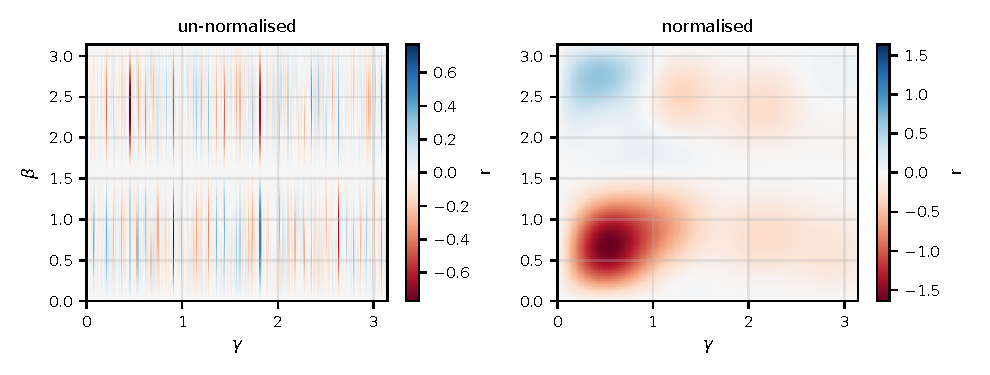
\includegraphics[width=0.92\linewidth]{figures/qaoa_landscape.pdf}
\caption{Exact approximation ratio $r(\gamma,\beta)$ at depth 1 on a
$257\times128$ grid. Left: cost Hamiltonian in problem units.
Right: divided by its largest coefficient. The two panels show the
same function; the left one samples it at $\gamma$ scaled by
$9\times10^{4}$.}
\label{fig:qaoa-landscape}
\end{figure}

\paragraph{Why the Hamiltonian is normalised.}
Figure~\ref{fig:qaoa-landscape} shows what an
optimiser sees without and with normalisation. With the Hamiltonian in problem
units, $r$ at neighbouring grid points along $\gamma$ is uncorrelated
(Pearson $-0.11$; normalised: $1.00$): at the optimiser's step size the
landscape is noise with standard deviation $0.10$. Good points exist in it
(the grid maximum is $0.54$), but a local search cannot find them. Training
in problem units is a random search over 60 points.

\begin{table}[H]
\centering\footnotesize\setlength{\tabcolsep}{3.5pt}
\begin{tabular}{lcccc}
\toprule
Arm & $p$ & Ratio $r$ & Constraint-satisfying & Ground level in 1\,024 shots \\
\midrule
Uniform sampling (exact) & --- & 0 & 0.079\% & 0.8\% \\
\midrule
Un-normalised, platform training & 1 & $0.180 \pm 0.042$ & 0.11\% & 0.6\% \\
 & 2 & $0.222 \pm 0.043$ & 0.26\% & 2.8\% \\
 & 3 & $0.167 \pm 0.035$ & 0.21\% & 0.5\% \\
Normalised, platform training & 1 & $0.199 \pm 0.127$ & 0.73\% & 12\% \\
 & 2 & $0.290 \pm 0.107$ & 1.35\% & 23\% \\
 & 3 & $0.304 \pm 0.103$ & 1.56\% & 24\% \\
Normalised, shipped sampler & 1 & $0.176 \pm 0.116$ & 0.76\% & 14\% \\
 & 2 & $0.175 \pm 0.088$ & 0.88\% & 16\% \\
 & 3 & $0.312 \pm 0.112$ & 3.04\% & 28\% \\
\midrule
Normalised, exact objective, best of 50 & 1 & 0.657 & 2.70\% & 46\% \\
 & 2 & 0.770 & 6.07\% & 81\% \\
 & 3 & 0.826 & 15.0\% & 99\% \\
\bottomrule
\end{tabular}
\caption{QAOA on an 18-qubit facility-location QUBO, every final state
evaluated exactly. Trained arms: mean over 20 seeds, with a 95\% interval
for $r$. The first two trained arms emulate the platform's training
procedure with and without normalisation; the third is the shipped sampler
itself.}
\label{tab:qaoa}
\end{table}

\begin{figure}[H]
\centering
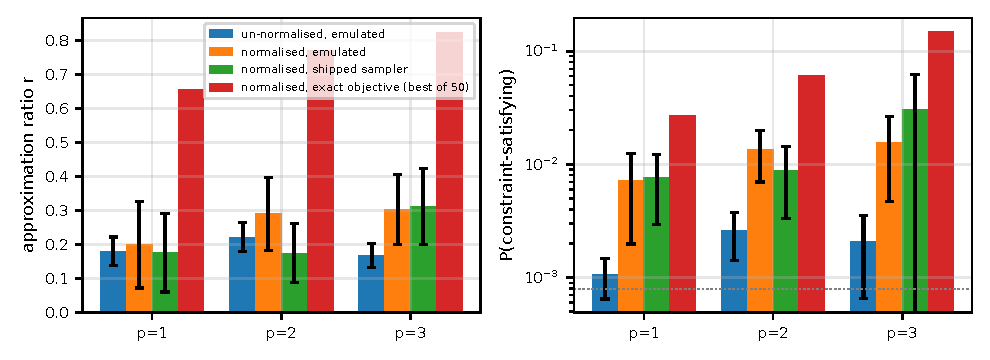
\includegraphics[width=0.92\linewidth]{figures/qaoa_exact.pdf}
\caption{Approximation ratio (left) and probability of a
constraint-satisfying sample (right, logarithmic; dotted: uniform) for the
arms of Table~\ref{tab:qaoa}. Bars: mean over 20 seeds with 95\% intervals;
the exact-objective arm is a single best value.}
\label{fig:qaoa}
\end{figure}

\paragraph{What the trained states are.} Without normalisation the trained
state has $r = 0.17$--$0.22$, above uniform in all 60 runs, but puts only
1.4--3.3 times the uniform probability on constraint-satisfying states, and
1\,024 shots contain the ground level with probability $0.5$--$2.8\%$,
against $0.8\%$ for uniform sampling (Table~\ref{tab:qaoa}). With
normalisation and the same training budget, the mean of $r$ rises but its
distribution does not shift reliably (one-sided Mann--Whitney $p = 0.98$,
$0.38$, $0.022$ at depth 1, 2, 3; the last does not survive a correction for
three tests): $r$ varies widely between seeds, with medians of
$0.07$--$0.25$. The constraint-satisfying probability rises
to 9--20 times uniform (same test: $p = 0.13$, $7\times10^{-4}$,
$1\times10^{-6}$) and
1\,024 shots contain the ground level with probability 12--24\%. The shipped
sampler agrees with
its emulation: of six two-sided comparisons the smallest $p$ is $0.044$ ($r$
at depth 2), the others at least $0.24$.

\paragraph{What the ansatz can do.} Minimising the exact expectation with
L-BFGS-B from 50 random starts in $[0,\pi]^{2p}$, all converged, gives
$r = 0.66$, $0.77$ and $0.83$ at depth 1, 2 and 3. At depth 1 the grid of
Figure~\ref{fig:qaoa-landscape} confirms the optimum inside the
initialisation box without an optimiser ($0.657$). At depth 3 the state puts
15\% of its probability on constraint-satisfying assignments, 189 times the
uniform share, and 1\,024 shots contain the ground level with probability
99\%. The true optimum is found almost as often as the ground level
($0.48\%$ against $0.50\%$ per shot at depth 3). The landscape is rugged:
only 13, 5 and 2 of the 50 starts end within 0.01 of the best value, and
the median start reaches $0.10$, $0.36$ and $0.50$. The best values are
therefore lower bounds on what the ansatz can reach.

\paragraph{What limits the sampler.} With adequate parameters, quality
grows with depth. What limits the
shipped sampler is training: 60 noisy evaluations from one random start
reach less than half of what the ansatz offers. Training on the exact
expectation where the register fits in memory, several starts, and parameter
transfer~\cite{shaydulin2023} are the obvious improvements. The scope of the
result is narrow: one instance, noiseless, with parameters found by a
classical simulation of the full state. A penalised one-hot landscape
remains a hard case for transverse-field mixers, and constraint-preserving
mixers~\cite{hadfield2019} are the natural next test.

\finding{A variational method that looks no better than random may be badly
scaled or badly trained. Before reporting a negative result, evaluate the
state exactly where the size allows, and separate what the ansatz can reach
from what the training procedure finds.}

\subsection{Portfolio selection: a selection is not yet a portfolio}
\label{sec:res-portfolio2}

\inbrief{Four gate-model methods select assets by minimising a QUBO. Each
is measured against the exact minimum of the QUBO it builds and against a
null that pushes uniform bits through the same code. On 30 instances that no earlier run had
touched, QAOA returns an exact optimum in 50, 43 and 39 of 50 runs at 8, 12
and 16 assets, against 21, 3 and 0 for its null, and the result holds on a
second instance family. CVaR-VQE beats its null only without a cap on the
number of assets. BF-DCQO and PCE with a cap return the optimum in every
run, and so do their nulls: the classical search that follows the sampling
finds it from any start at these sizes. Followed to the screen, the
portfolio displayed is the one the classical weighting computes without any
selection in 138 of 150 QAOA runs.}

Portfolio selection is the workload the platform was built around. Its
classical baseline returns continuous maximum-Sharpe weights, while every
quantum method selects a subset of assets by minimising a QUBO, so the
baseline is no referee for the selection. At 8--16 assets the exact answer
is an enumeration of $2^n$ selections, which takes $0.1$--$4$\,ms.
CVaR-VQE, BF-DCQO and PCE follow the papers they are named
after~\cite{barkoutsos2020,cadavid2024,cadavid2026,sciorilli2024}, each
with tests of the step that defines it; QAOA returns the cheapest of its
final samples; every method takes a seed; and
each result carries the exact standing of the returned selection among the
selections the method may return (Table~\ref{tab:pf-corrected}). We
measured the four methods against that referee and against nulls on 30
instances that an earlier experiment had used
(E20), and then tested the one positive result on 30 instances that no
earlier run had touched (E21), on 30 instances of a second family (E23) and
on hardware (E22, Section~\ref{sec:res-hw3}); E25 compared two starting
points of its training. Last, we followed that result
to what the product displays (E24).

\begin{table}[H]
\centering\footnotesize\setlength{\tabcolsep}{4pt}
\begin{tabular}{p{1.6cm}p{4.5cm}p{4.3cm}p{3.8cm}}
\toprule
Method & Objective built & Selection returned & Simulator defaults \\
\midrule
QAOA & $-\mu^\top x + \tfrac12\,x^\top S x$; no cardinality term & Lowest-cost of 200 final samples & 15 evaluations of 100 shots, depth 2 \\
CVaR-VQE & $-\mu^\top x + \tfrac12\,x^\top\Sigma x$, plus $2.5\,(\mathbf 1^\top x - K)^2$ when the user caps the number of assets at $K$ & Lowest-cost of 2\,048 final samples that holds $K$ assets (at least one asset without a cap) & Mean of the lowest quarter of 1\,024 sampled energies; up to $10\,(P+1)$ evaluations for $P$ parameters; depth 2 \\
BF-DCQO & $-\tfrac12\,\mu^\top x + \tfrac12\,x^\top\Sigma x + \Lambda(\mathbf 1^\top x - K)^2$ & Best samples of each cluster of $\le 8$ qubits and of each iteration, recombined across clusters, each passed through cardinality repair and a swap search; the cheapest under the QUBO & $3 \times 8\,192$ shots per cluster; depth 2, that is one counterdiabatic layer \\
PCE & as CVaR-VQE, with the penalty weight set from the coefficients of the QUBO & Signs of the measured Pauli correlators, then single-bit flips and, with a cap, swaps under the QUBO & 3, 4 and 6 qubits for 8, 12 and 16 assets; 72 loss evaluations of 1\,024 shots in each of three bases \\
\bottomrule
\end{tabular}
\caption{What the four portfolio methods compute, and the simulator
defaults their worker executors read from one table. $K$ is the user's cap
on the number of assets. Where a source states its method for another
problem or leaves a choice open, the choice is ours: for BF-DCQO the norm in
the counterdiabatic coefficient, the initial state and the time grid, on
which the last step carries no rotation, so that a circuit of depth $d$ has
$d-1$ counterdiabatic layers; for PCE the linear term of the loss, the scale
of its regulariser, the swap step and the training schedule. We do not claim
to reproduce the results of those papers.}
\label{tab:pf-corrected}
\end{table}

\paragraph{Design.} Seeded synthetic price series from a factor model (504
trading days), 10 instances at each of
8, 12 and 16 assets, 5 seeds per instance. Each method is refereed against
the exact minimum over all $2^n$ selections of
the QUBO it builds itself, because the four build four different ones. Each
is paired with a \emph{null} that pushes uniform bits through the same
platform code, so that objective evaluation, optimiser, sampling, selection
rule, repair and refinement all run unchanged: for QAOA and
CVaR-VQE the ansatz is replaced by a Hadamard layer followed by
parameterised $Z$ rotations, whose measured distribution is uniform for
every parameter value; for BF-DCQO
uniform counts take the place of the sampler's; for PCE the correlators are
computed from
uniform counts in all three bases. The measures are the share of runs that
return an exact optimum, the share of the selections a method may return
that are cheaper than the returned one, and the gap
$g = (c - c_{\min})/(\bar c - c_{\min})$, which is 0 at the optimum and 1
for the average selection. The test is the gap of a method against its
null, paired by instance (Wilcoxon signed-rank).
CVaR-VQE and PCE are run with a cap of
$K = \lfloor n/3\rfloor$ assets, the value BF-DCQO uses, and without one.
There are seven arms and 21 primary comparisons, so the corrected threshold
is $0.0024$; with ten instances the smallest $p$-value the test can return
is $0.0020$. The instances of E20 had been used by an earlier experiment,
so E20 is not an independent test, which is why E21 exists.

The budgets of CVaR-VQE and PCE were tuned on
held-out instances in two grids: 36 configurations with 8 runs per cell
(1\,728 runs), then a follow-up with ten seeds (1\,920 runs) whose decision
rules were written into the script before it ran. The first grid ranked 256
shots above 1\,024 for PCE; with ten seeds the difference had the opposite
sign ($0.09$, standard error $0.06$), and the defaults follow the second
grid. The tuning also showed that BF-DCQO and PCE with a cap return the
optimum from uniform samples in every configuration, because the classical
search that follows the sampling finds it from any start at these sizes.
Before any evaluation run we therefore added a secondary family of 21
comparisons on what the circuits deliver \emph{before} that search
(Table~\ref{tab:portfolio2b}), with its own threshold of $0.0024$. The
evaluation was run twice from committed code: the 3\,000 runs agree in every
field except run time, and none failed.

\begin{table}[H]
\centering\footnotesize\setlength{\tabcolsep}{4pt}
\begin{tabular}{lrccccl}
\toprule
 & & \multicolumn{2}{c}{Exact optimum returned} & \multicolumn{2}{c}{Better selections (\%)} & \\
Method & $n$ & method & null & method & null & $p$ \\
\midrule
QAOA & 8 & 49/50 & 35/50 & $0.01 \pm 0.02$ & $0.18 \pm 0.09$ & 0.0039 \\
 & 12 & 42/50 & 2/50 & $0.01 \pm 0.01$ & $0.54 \pm 0.13$ & 0.0020 \\
 & 16 & 38/50 & 0/50 & 0 & $0.46 \pm 0.22$ & 0.0020 \\
CVaR-VQE, no $K$ & 8 & 50/50 & 50/50 & 0 & 0 & tie \\
 & 12 & 46/50 & 20/50 & $0.01 \pm 0.01$ & $0.04 \pm 0.02$ & 0.0020 \\
 & 16 & 44/50 & 0/50 & $0.01 \pm 0.02$ & $0.06 \pm 0.02$ & 0.0020 \\
CVaR-VQE, $K$ & 8 & 44/50 & 50/50 & $0.79 \pm 0.95$ & 0 & 0.12 \\
 & 12 & 23/50 & 18/50 & $0.55 \pm 0.35$ & $0.29 \pm 0.08$ & 0.56 \\
 & 16 & 5/50 & 2/50 & $1.09 \pm 0.80$ & $0.64 \pm 0.28$ & 0.85 \\
BF-DCQO & 8--16 & 150/150 & 150/150 & 0 & 0 & tie \\
BF-DCQO, 32 shots & 8--16 & 150/150 & 150/150 & 0 & 0 & tie \\
PCE, no $K$ & 8 & 45/50 & 43/50 & $0.04 \pm 0.06$ & $0.05 \pm 0.08$ & 1.00 \\
 & 12 & 50/50 & 50/50 & 0 & 0 & tie \\
 & 16 & 45/50 & 45/50 & 0 & 0 & 1.00 \\
PCE, $K$ & 8--16 & 150/150 & 150/150 & 0 & 0 & tie \\
\midrule
QAOA, new instances & 8 & 50/50 & 21/50 & 0 & $0.34 \pm 0.11$ & 0.0020 \\
 & 12 & 43/50 & 3/50 & $0.01 \pm 0.02$ & $0.44 \pm 0.17$ & 0.0020 \\
 & 16 & 39/50 & 0/50 & 0 & $0.45 \pm 0.16$ & 0.0020 \\
\bottomrule
\end{tabular}
\caption{The selections the methods return, against the exact
optimum of each method's own QUBO and against a null that runs uniform bits
through the same code. ``Better selections'': share of the selections the
method may return (those with exactly $K$ assets, or all of them without a
cap) that are cheaper than the returned one; means with 95\% intervals over
10 instances (5 seeds each). $p$: Wilcoxon signed-rank test on the gap
$g$, unadjusted, to be compared with $0.0024$
(E20, above the rule) and $0.017$ (E21, below it); ``tie'': method and null
had the same gap on every instance. Rows marked 8--16 pool the three sizes.
For the null of the last three rows exact uniform sampling predicts 27.1,
2.4 and 0.2 optimal runs.}
\label{tab:portfolio2}
\end{table}

\paragraph{QAOA.} The returned selection, the cheapest of 200 final
samples, is an
exact optimum in 49, 42 and 38 of 50 runs at 8, 12 and 16 assets, against
35, 2 and 0 for uniform
samples read by the same rule (Table~\ref{tab:portfolio2}). At 8 assets the
comparison does not pass the corrected threshold: one instance ties, and
nine instances cannot return less than $p = 0.0039$. At that size 200
uniform samples contain the single optimum with probability $0.54$, and the
null returned it in 35 runs where 27.1 are expected. A further 1\,000 null
runs with other seeds returned it in 543 against 542.9 expected: the 35 were
chance, and the null is calibrated.

On the 30 new instances (E21), run through the product's own seed argument
with nothing substituted around the product code except the ansatz of the
null, the method returned an optimum in 50, 43 and 39 of 50 runs against 21,
3 and 0 for the null. Its gap was the lower one on 10 of 10 instances at
every size ($p = 0.0020$ each; three comparisons, threshold $0.017$). The
trained state holds the optimum with 16, 75 and 441 times its uniform
probability (medians) at approximation ratios of $0.63$, $0.65$ and $0.73$.
The selected sample was also the most frequent one in only 20, 8 and 6 of
the 50 runs, which is why the method returns the cheapest sample and not
the most frequent one.

E20 and E21 share one instance generator. A default run from the product's
panel uses another, the gateway's simulated market data: 90 days of history
instead of 504, and a cost function that its linear terms dominate more
strongly (largest linear over largest pair coefficient 18 to 25, against 9
to 10) and that spans $1.9$, $2.9$ and $4.2$ times $\pi$ instead of $0.5$,
$0.7$ and $1.3$. While the deployed panel was being checked, one such run
returned a selection with 8 cheaper alternatives among 256. E23 therefore
repeated E21 on 30 instances from that generator; its design was committed
before the run, after a harness check had shown 8 of its 300 runs. The
result of E21 holds: an optimum in 49, 45 and 43 of 50 runs against 31, 1
and 0 for the null, and a lower gap on 8, 9 and 10 of 10 instances (two
ties at 8 assets, one instance worse at 12; $p = 0.0078$, $0.0039$,
$0.0020$; threshold $0.017$). The run that prompted the experiment was on
the panel's default instance. Examined afterwards with 20 seeds, outside
the design, that instance returned the optimum in 13 runs and a selection
with 5 to 15 cheaper alternatives in 5, where 200 uniform samples leave
$0.84$ on average. What E21 and E23 measure is an average over instances.
It is not a property of every run, which is what the reference attached to
each result is for.

\paragraph{The start of the training.} The QAOA path starts its training
from two linear ramps over the layers, one rising from $\pi/8$ to $\pi/2$
and one falling from $\pi/2$ to $\pi/8$. With the product's
two layers the training starts at $\beta = (\pi/8, \pi/2)$ and
$\gamma = (\pi/2, \pi/8)$. Every QAOA result in this paper was measured with
that start. E25 compared it with the opposite assignment of the two ramps,
$\gamma$ rising and $\beta$ falling, on the instances
and seeds of E21 and E23, with two outcomes, twelve comparisons and a
decision rule committed and pushed before the run. The product's arm returned
the stored results of E21 and E23 in 300 of 300 runs
(Table~\ref{tab:initial-angles}). The opposite start was better in no
comparison and worse in four, all on the instances of E21: its trained
states have lower approximation ratios at all three sizes, and at 16 assets
it returned worse selections, an optimum in 25 of 50 runs against 39. On the
product's data no comparison passed the threshold. At its initial angles the
opposite start is worse than uniform sampling in every cell, the product's
one better. By the rule fixed in advance the product keeps its start.
Neither was tuned, and no third was
tried. The angles depend on
the number of layers only, not on a classical solution of the instance.

\begin{table}[H]
\centering\footnotesize\setlength{\tabcolsep}{4pt}
\begin{tabular}{llcccccccccc}
\toprule
 & & \multicolumn{2}{c}{Optimal runs} & \multicolumn{2}{c}{Returned selection} & \multicolumn{4}{c}{Final state, approx.\ ratio} & \multicolumn{2}{c}{Initial ratio} \\
Instances & $n$ & opp. & product & b/w/t & $p$ & opp. & product & b/w/t & $p$ & opp. & product \\
\midrule
E21 & 8 & 49/50 & 50/50 & 0/1/9 & 1.00 & 0.47 & 0.63 & 0/10/0 & 0.0020 & $-0.24$ & 0.28 \\
 & 12 & 31/50 & 43/50 & 0/7/3 & 0.016 & 0.54 & 0.65 & 1/9/0 & 0.0039 & $-0.26$ & 0.29 \\
 & 16 & 25/50 & 39/50 & 0/9/1 & 0.0039 & 0.58 & 0.73 & 0/10/0 & 0.0020 & $-0.36$ & 0.38 \\
E23 & 8 & 49/50 & 49/50 & 1/1/8 & 1.00 & 0.63 & 0.61 & 5/5/0 & 1.00 & $-0.53$ & 0.39 \\
 & 12 & 42/50 & 45/50 & 2/3/5 & 0.81 & 0.58 & 0.58 & 3/7/0 & 0.43 & $-0.50$ & 0.34 \\
 & 16 & 37/50 & 43/50 & 0/5/5 & 0.062 & 0.61 & 0.67 & 3/7/0 & 0.11 & $-0.53$ & 0.37 \\
\bottomrule
\end{tabular}
\caption{E25: the start of the training with the two ramps assigned the
other way round (``opp.'') against the start the product uses
(``product''), on the instances
and seeds of E21 and E23; 50 runs per cell and arm. b/w/t: instances on
which the opposite start is better, worse or tied, by per-instance mean.
$p$: Wilcoxon signed-rank, two-sided, unadjusted; twelve comparisons,
threshold $0.0042$. Approximation ratios are those of the exact final and
initial states, as means over instances; a negative ratio is worse than
uniform sampling.}
\label{tab:initial-angles}
\end{table}

\paragraph{CVaR-VQE.} Without a cap the method returns an optimum
in 50, 46 and 44 of 50 runs. At 8 assets so does its null, and the
comparison ties: 2\,048 uniform samples contain a single optimum among 256
selections with probability $0.9997$. At 12 and 16 assets the null returns
it in 20 and 0 runs, and the method is better on 10 of 10 instances
($p = 0.0020$). The trained state holds the optimum with 69, 1\,050 and
15\,731 times its uniform probability (medians).

With a cap the method is not better than uniform sampling under the same
rule. It returned an optimum in 44, 23 and 5 runs against 50, 18 and 2 for
the null ($p = 0.12$, $0.56$, $0.85$), and among the selections of exactly
$K$ assets its returned selection left on average more cheaper alternatives
than the null's ($0.8$, $0.5$ and $1.1\%$ against $0$, $0.3$ and $0.6\%$).
Training does move the state towards the cap: $44$, $34$ and $17\%$ of the
final shots hold exactly $K$ assets, against $11$, $12$ and $6.5\%$ for
uniform bits. It does not move it towards the optimum: the trained state
holds the optimum with 63, $0.54$ and $0.15$ times its uniform probability
(medians), at 12 and 16 assets less than a uniform state. The minimum of the
QUBO holds $K$ assets in every run, so the cap is encoded correctly; why
training does not find the optimum within it we have not established. The
product returns such a result with the exact reference attached, which
states for the run how many selections are cheaper and what uniform sampling
would have given.

\paragraph{BF-DCQO and PCE: the classical search decides.} For BF-DCQO, at
the executor's 8\,192 shots and at 32 shots per iteration, and for PCE with
a cap, method and null return the exact optimum in 150 of 150 runs each. For
PCE without a cap they return it in 140 and 138 of 150. At these sizes the
returned selection says nothing about the circuit: the repair, flip and swap
searches that follow the sampling reach the optimum from uniform samples.

\begin{table}[H]
\centering\footnotesize\setlength{\tabcolsep}{4pt}
\begin{tabular}{lrccccl}
\toprule
 & & \multicolumn{2}{c}{Exact optimum} & Gap, first & Instances & \\
Compared & $n$ & first & second & minus second & $-$ / $+$ / $=$ & $p$ \\
\midrule
PCE decoded, no $K$ & 8 & 3/50 & 0/50 & $-0.80 \pm 0.14$ & 10/0/0 & 0.0020 \\
 & 12 & 0/50 & 0/50 & $-0.42 \pm 0.16$ & 10/0/0 & 0.0020 \\
 & 16 & 0/50 & 0/50 & $-0.26 \pm 0.21$ & 8/2/0 & 0.027 \\
PCE decoded, $K$ & 8 & 1/50 & 0/50 & $-0.75 \pm 0.38$ & 9/1/0 & 0.0039 \\
 & 12 & 0/50 & 0/50 & $-0.83 \pm 0.30$ & 10/0/0 & 0.0020 \\
 & 16 & 0/50 & 0/50 & $-0.48 \pm 0.48$ & 7/3/0 & 0.037 \\
\midrule
BF-DCQO shots, depth 1 & 8 & 30/50 & 17/50 & $-0.0087 \pm 0.0096$ & 7/3/0 & 0.084 \\
 & 12 & 6/50 & 1/50 & $-0.0058 \pm 0.0085$ & 6/4/0 & 0.19 \\
 & 16 & 0/50 & 1/50 & $-0.0048 \pm 0.0024$ & 9/1/0 & 0.0039 \\
BF-DCQO shots, depth 2 & 8 & 34/50 & 14/50 & $-0.0094 \pm 0.0069$ & 9/1/0 & 0.020 \\
 & 12 & 3/50 & 2/50 & $-0.0105 \pm 0.0048$ & 9/1/0 & 0.0039 \\
 & 16 & 0/50 & 0/50 & $-0.0042 \pm 0.0061$ & 7/3/0 & 0.23 \\
BF-DCQO shots, depth 3 & 8 & 46/50 & 17/50 & $-0.0120 \pm 0.0064$ & 10/0/0 & 0.0020 \\
 & 12 & 14/50 & 4/50 & $-0.0211 \pm 0.0101$ & 9/1/0 & 0.0039 \\
 & 16 & 1/50 & 0/50 & $-0.0086 \pm 0.0032$ & 10/0/0 & 0.0020 \\
\midrule
depth 2 against depth 1 & 8 & & & $-0.0038 \pm 0.0063$ & 7/2/1 & 0.16 \\
 & 12 & & & $-0.0050 \pm 0.0097$ & 9/1/0 & 0.084 \\
 & 16 & & & $0.0030 \pm 0.0040$ & 2/8/0 & 0.13 \\
depth 3 against depth 1 & 8 & & & $-0.0056 \pm 0.0048$ & 8/1/1 & 0.0078 \\
 & 12 & & & $-0.0116 \pm 0.0071$ & 10/0/0 & 0.0020 \\
 & 16 & & & $-0.0036 \pm 0.0030$ & 7/3/0 & 0.049 \\
\bottomrule
\end{tabular}
\caption{What the circuits deliver before the classical search. Upper and
middle block: the method (first) against its uniform null (second). PCE:
the selection decoded from the signs of the measured correlators. BF-DCQO:
the lowest-energy raw shot over all iterations, with one cluster holding
all assets and 32 shots per iteration. Lower block: depths 2 and 3 against
depth 1, whose circuit contains no counterdiabatic rotation and is the
control for the bias feedback. Differences of the gap $g$ (negative: the
first is closer to the optimum), means with 95\% intervals over 10
instances; instances on which the first is better, worse or equal; $p$:
Wilcoxon signed-rank test, unadjusted, to be compared with $0.0024$.}
\label{tab:portfolio2b}
\end{table}

What the circuits contribute shows only before that search
(Table~\ref{tab:portfolio2b}). The selection that PCE decodes from the signs
of its measured correlators is closer to the optimum than one decoded from
uniform counts on 10, 10 and 8 of 10 instances without a cap and on 9, 10
and 7 with one; three of the six comparisons pass the corrected threshold.
The decoded selection is itself an optimum in 4 of 300 runs. The classical
search then changes $1.8$ to $7.5$ of its bits on average, depending on
size and cap, against $4.0$ to $8.0$ for the null. PCE does this with 3, 4
and 6 qubits for 8, 12 and 16 assets.

For BF-DCQO the circuit has to be separated from the bias feedback, which is
classical: the bias fields of an iteration are computed from shots that
classical sweeps have lowered. The control is the circuit of depth 1, which
on our time grid contains no counterdiabatic rotation, so that every
iteration samples the product state its bias fields prepare. Against
uniform counts this control alone is better on 7, 6 and 9 of 10 instances.
The best raw shot at the executor's default depth 2, one counterdiabatic
layer, is not distinguishable from the control ($p = 0.16$, $0.084$,
$0.13$; at 16 assets it is the worse one on 8 of 10 instances). At depth 3,
two layers, it is better than the control on 8, 10 and 7 of 10 instances
($p = 0.0078$, $0.0020$, $0.049$), and the comparison at 12 assets passes
the corrected threshold. Evaluated exactly at zero bias, the depth-2
circuit holds the optimum with $0.15$, $0.31$ and less than $0.01$ times
its uniform probability (medians), the depth-3 circuit with $2.2$, $3.1$
and $0.49$ times. The source uses two time steps. Whether they correspond
to our depth 2 or to our depth 3 depends on the time grid, which is our
choice (Table~\ref{tab:pf-corrected}), and we draw no conclusion about the
published method.

\paragraph{From the selection to the displayed portfolio.} Everything above
scores the selection a method returns. The product displays weights and key
figures, and between the two the QAOA executor runs three classical steps:
minimum-variance weights on the selected assets; a long-only mean--variance
program on the assets that keep a positive weight, which minimises
$J(w) = \tfrac12\,w^\top\Sigma w - \mu^\top w$ with at most 40\% per asset
and a cap on the Herfindahl index; and, if the result is still concentrated,
a replacement by the minimum-variance portfolio of the five assets with the
highest Sharpe ratio. On the panel's default instance two QAOA runs and three
runs of the annealing methods displayed the same allocation to two decimals.
E24 asks whether that is general. It calls the executor itself, as the worker
does for a default run without a limit on the number of assets, on the 30
instances of E23, in five arms: the method and its null, with the seeds of
E23 (all 300 runs returned the selections scored there), and three selections
put in the place of the quantum result: every asset, which leaves the
classical steps alone; the exact optimum of the QUBO; and uniform selections,
all 255 at 8 assets and 1\,000 per instance at 12 and 16. The design, two
tests on $J$ of the displayed weights and the conclusion each outcome would
lead to were committed before the run.

\begin{table}[H]
\centering\footnotesize\setlength{\tabcolsep}{3pt}
\begin{tabular}{rcccrrrrclcl}
\toprule
 & \multicolumn{4}{c}{Display as without a selection} & Worse & \multicolumn{2}{c}{Assets} & \multicolumn{2}{c}{$J$ against null} & \multicolumn{2}{c}{$J$ against none} \\
$n$ & QAOA & null & optimum & uniform (\%) & $J$ (\%) & selected & held & $-$/$+$/$=$ & $p$ & $-$/$+$/$=$ & $p$ \\
\midrule
8 & 40/50 & 39/50 & 8/10 & 9.41 & 90.59 & 5.1 & 3.8 & 2/1/7 & 0.50 & 0/2/8 & 0.50 \\
12 & 48/50 & 46/50 & 10/10 & 6.35 & 93.65 & 7.5 & 3.9 & 2/1/7 & 0.50 & 0/1/9 & 1.00 \\
16 & 50/50 & 46/50 & 10/10 & 6.55 & 93.45 & 10.3 & 4.2 & 3/0/7 & 0.25 & 0/0/10 & tie \\
\bottomrule
\end{tabular}
\caption{What a default QAOA run displays (E24; the product's executor on the
30 instances of E23). ``Display as without a selection'': runs, instances or
share of uniform selections whose displayed allocation is the one the
classical steps produce when every asset is selected (no weight differs by
more than $0.0005$). ``Worse $J$'': share of uniform selections whose
displayed allocation has a higher $J$ than that one; none has a lower one.
Shares are medians over 10 instances. ``Assets'': assets in the QAOA
selection, and positions above 1\% in what is displayed (means). Tests: $J$
of the displayed weights of QAOA against that of its null and against that
of no selection, per-instance means; instances on which QAOA is lower,
higher or tied; Wilcoxon signed-rank, two-sided, unadjusted, to be compared
with $0.0083$; ``tie'': equal on every instance.}
\label{tab:displayed}
\end{table}

The displayed allocation was the one the classical steps produce alone in
40, 48 and 50 of 50 QAOA runs, in 39, 46 and 46 of 50 null runs, and for the
exact optimum of the QUBO on 8, 10 and 10 of 10 instances
(Table~\ref{tab:displayed}). Neither test separates anything. By the rules
stated in advance, nothing is concluded at any size: not that the selection
reaches the user, and not that the selection step improves or worsens what
is displayed.

The reason lies in the construction, and the design should have named it.
The second step minimises $J$ over the assets the first step leaves with a
positive weight. With every asset selected, the first step kept every asset
on all 30 instances (checked after the run), so the classical steps alone
minimise $J$ over the whole universe and a selection can only restrict that
program: on $J$ the selection step can at best change nothing, and the
second test could only have shown harm. Of 22\,550 uniform selections none
displayed a lower $J$ than the classical steps alone, and more than nine in
ten displayed a higher one. Where the QAOA display differs (two instances at
8 assets, in all five runs each; one at 12 assets, in two runs), its $J$ is
higher by $0.0033$ and $0.0012$, or by less than $10^{-5}$, and no weight
differs by more than $2.1$ percentage points. The Sharpe
ratio, which no step optimises, was the secondary outcome and could have
moved either way. It did not: $3.313$, $3.424$ and $3.710$ for QAOA against
$3.314$, $3.424$ and $3.710$ without a selection, and no test below
$p = 0.46$.

That QAOA and its null end at the same display, while a uniform selection
does so in 6 to 9\% of cases, has a simple cause. The QUBO cost of a
selection and the $J$ of what is displayed for it are rank-correlated
(Spearman, medians $0.71$, $0.89$ and $0.86$): a cheap selection contains
the assets the mean--variance step would hold, and holds more of them than
the step keeps ($5.1$, $7.5$ and $10.3$ selected against $3.8$, $3.9$ and
$4.2$ positions above 1\%). The cheapest of 200 uniform samples is cheap
enough for that. The null returns an optimum of the QUBO in 31, 1 and 0 of
50 runs and still ends at the same display in 39, 46 and 46.

E21 to E23 measure a property of the selection under the method's own cost,
and they stand. On the default path of the product that property does not
reach the user: the portfolio on the screen is the one the classical steps
compute without a selection, or one that is slightly worse by their
objective. Each QAOA result states which of the two it is, with the
allocation of the classical steps alone next to it. Four limits apply. One
method was measured; the executors of the other three end in the same second
and third step after a first step of their own. The instances are one
family. No limit on the number of assets was set; with one, the executor
first cuts the pool down classically and the selection then restricts that
pool. And $J$ and the Sharpe ratio are in-sample figures on 90 days of
simulated prices, which say nothing about how any of these portfolios would
perform. A selection can matter for the display only where the weighting
step cannot solve the problem itself, for example when exactly $K$ assets
must be held and the unconstrained weights hold more. That experiment has
not been run (Section~\ref{sec:agenda}).

\paragraph{What the product states.} Every result of the four methods
carries an exact reference, computed by the enumeration used here for up to
20 assets: the number of selections the method may return, how many of them
are cheaper than the returned one and, for the methods that return the
cheapest of $S$ samples, the exact probability that $S$ uniform samples
would have returned an optimum. The reference agreed with the scoring of the
experiments in all 3\,000 runs of E20 and all 300 of E21.

A run started from the interface uses the simulator defaults of
Table~\ref{tab:pf-corrected}: the
gateway fills in nothing for simulator runs of the four methods, the
interface's simulator presets are a copy of the measured table that a test
compares with it option by option, and its panels offer only options the
back-end reads. Presets for
hardware runs are cost caps and were not measured, and neither were the
caps that the assistant sends per run-quality tier.

\finding{Measured against the exact optimum and
against uniform bits through the same code, one of four methods returns better selections
than chance, one does so only without a cardinality cap, and two reach the
optimum through a classical search that reaches it from random samples as
well. A product can say this per result: where the answer stands exactly,
and what uniform sampling would have given. A selection that is better than
chance is still not a better portfolio: on the product's default path the
classical weighting that follows displays the same allocation with the
selection and without it.}

\subsection{Vehicle routing}
\label{sec:res-fleet}

\inbrief{Two presets of 90 and 120 stops, ten generated instances each and
five sampler seeds per instance: two simulated annealers on the assignment
QUBO against the platform's classical construction. The annealing pipelines
are 13--60\% longer on average. Every run with a shorter distance left more
stops unserved, and three of 200 runs won on the full objective, where the
heuristic referee itself had dropped stops.}

Two presets (90 stops, 12 vehicles; 120 stops, 18 vehicles), ten
independently generated instances each, five sampler seeds per instance.
Simulated annealing on the assignment QUBO (\texttt{neal}) and a NumPy
annealer, against the platform's classical construction on the same
instance. Runs on one instance share that instance, so the unit of analysis
is the instance (Table~\ref{tab:fleet}).

\begin{table}[H]
\centering\small
\begin{tabular}{llrrrr}
\toprule
Instance & Sampler & Distance gap & Range over runs & Wins & Runs dropping stops \\
\midrule
90 stops & \texttt{neal} & $+13.4 \pm 3.4\%$ & $-6.7$ to $+37.8\%$ & 1/50 & 37/50 \\
90 stops & NumPy SA & $+15.2 \pm 8.4\%$ & $-12.9$ to $+50.7\%$ & 2/50 & 38/50 \\
120 stops & \texttt{neal} & $+59.9 \pm 6.2\%$ & $+27.3$ to $+87.7\%$ & 0/50 & 0/50 \\
120 stops & NumPy SA & $+51.4 \pm 7.2\%$ & $+23.9$ to $+92.4\%$ & 0/50 & 0/50 \\
\bottomrule
\end{tabular}
\caption{Routing: distance gap to the classical construction, mean over ten
instances of the per-instance mean, with a 95\% interval over instances.
``Wins'' compares the full objective, which penalises unserved stops; the
last column counts runs that left more stops unserved than the classical
construction.}
\label{tab:fleet}
\end{table}

The annealing pipelines are 13--60\% longer than the classical construction
on average, with a standard deviation of 10--15 points between sampler seeds
on one instance. All 13 runs with a negative distance gap left more stops
unserved than the referee,
a reminder that single-metric comparisons reward infeasibility.
Three of 200 runs won on the full objective, all on the 90-stop preset: each
served one to four more stops than the classical construction, at 5--31\%
more distance. The heuristic referee, in other words, itself dropped stops
on two instances.

\finding{At both sizes the classical construction gives the shorter plan on
average. A comparison on distance alone rewards infeasibility, and a
heuristic referee can lose on its own instance.}

\subsection{Spaced site selection on Rydberg arrays}
\label{sec:res-mis}

\inbrief{Does the static-radius mapping beat a mapping by the dynamic
radius? Local analog simulator of the ideal Rydberg Hamiltonian,
24 random 8-site instances per comparison. Against the dynamic-radius
mapping with an untuned sweep, the static mapping yields independent sets in $97\%$ of raw shots
against $41\%$. Against the same control with its sweep ratio tuned on
held-out instances, the raw optimal fraction is indistinguishable ($0.842$
against $0.832$, $p = 0.89$) and seven points of validity remain ($99.3\%$
against $92.6\%$). After greedy repair both reach the optimum on every
instance, and so does a greedy heuristic alone. Embeddability follows the
bound on the spacing ratio derived in Section~\ref{sec:workloads}: 93--100\%
of random instances embed below a ratio of $2.75$ and under 1\% above
$3.25$.}

Local Braket analog simulator, 4\,$\mu$s sweep, 200 shots per instance, every
simulation seeded. (a) 24 random 8-site instances with spacing ratios
$1.4$--$2.4$ relative to the closest pair, each run with the static-radius
mapping and with the dynamic-radius mapping swept
to $\Delta_{\mathrm{end}}/\Omega = 6$. (b) The same comparison against a
\emph{tuned} control: the sweep ratio of the dynamic-radius mapping is
chosen on 24 further instances and both mappings are compared on 24 more.
(c) Sweep duration $0.5$--$4\,\mu$s on the 10-city Rhine--Ruhr instance,
1\,000 shots per point. (d) Embeddability of 2\,000 random 10-site
instances.

\begin{figure}[H]
\centering
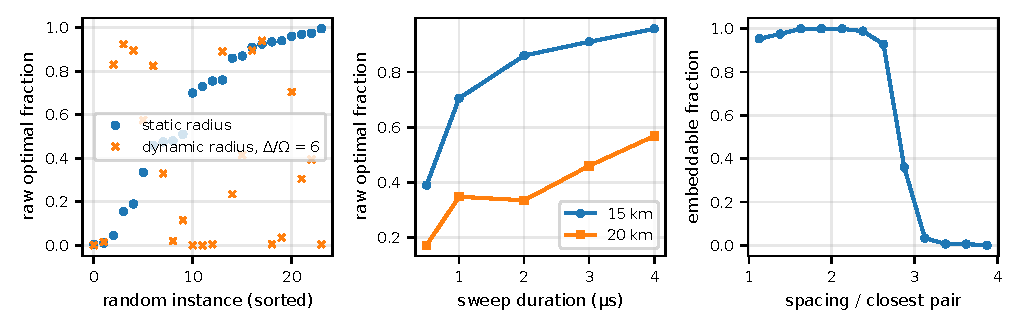
\includegraphics[width=\linewidth]{figures/rydberg_mis.pdf}
\caption{Left: fraction of raw shots that are optimal MIS on 24 random
instances, sorted, for the static-radius mapping and the untuned
dynamic-radius mapping. Centre: raw optimal fraction versus sweep duration on
the Rhine--Ruhr instance (15\,km: 6 conflicts; 20\,km: 10 conflicts). Right:
fraction of random instances that can be embedded versus the ratio of the
spacing rule to the closest-pair distance.}
\label{fig:mis}
\end{figure}

\begin{table}[H]
\centering\footnotesize\setlength{\tabcolsep}{4pt}
\begin{tabular}{lcccc}
\toprule
 & Dynamic, $\Delta_{\mathrm{end}}/\Omega = 6$ & Static & Paired difference & $p$ \\
\midrule
Raw shots that are independent sets & $40.7 \pm 16.9\%$ & $97.0 \pm 2.5\%$ & $+56.3 \pm 15.8$ & $2\times10^{-5}$ \\
Raw shots that are optimal & $39.0 \pm 16.0\%$ & $62.3 \pm 14.5\%$ & $+23.3 \pm 22.8$ & $0.056$ \\
Instances solved after repair & 24/24 & 24/24 & & \\
\bottomrule
\end{tabular}
\caption{(a) Static-radius mapping against the untuned
dynamic-radius mapping on 24 random instances (mean $\pm$ 95\% interval;
Wilcoxon signed-rank test). A greedy minimum-degree heuristic also solves all
24 exactly.}
\label{tab:mis}
\end{table}

\paragraph{Against the untuned control.} The static-radius mapping almost
always yields valid plans, the dynamic-radius mapping in 41\% of shots
(Table~\ref{tab:mis}). The mechanism is quantitative. A dynamic-radius
mapping that sweeps to $\Delta_{\mathrm{end}} = \rho\,\Omega$ has a static
radius of $\rho^{-1/6} R_b$ at readout: $0.74\,R_b$ at $\rho = 6$.
Conflicting pairs between $0.74$ and $1.0$ of the threshold are not
excluded once $\Omega$ is switched off, and both atoms are excited.

\begin{figure}[H]
\centering
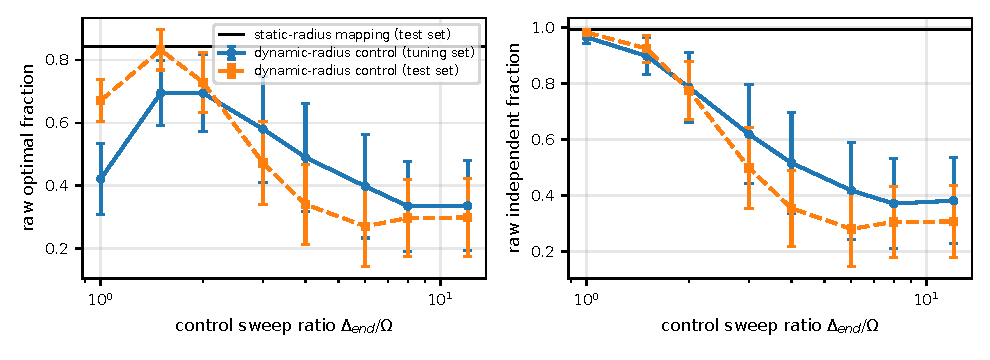
\includegraphics[width=0.92\linewidth]{figures/rydberg_tuned_control.pdf}
\caption{(b) The dynamic-radius control as a function of its sweep ratio, on
the tuning set and on the test set, against the static-radius mapping on the
test set (horizontal line). Left: raw optimal fraction, the tuning criterion.
Right: raw independent-set fraction. Means with 95\% intervals over 24
instances.}
\label{fig:mis-tuned}
\end{figure}

\paragraph{Against a tuned control.} That comparison is unfair to the
control, whose sweep ratio was never tuned. Tuned on 24 instances, its raw
optimal fraction peaks at $\rho = 1.5$ ($0.694$; $\rho = 2$ ties to three
digits). On 24 held-out instances the tuned control is indistinguishable
from the static-radius mapping in raw optimal fraction: $0.832 \pm 0.064$
against $0.842 \pm 0.086$, paired difference $+0.011 \pm 0.063$, Wilcoxon
$p = 0.89$, 13 instances against 11 (Figure~\ref{fig:mis-tuned}). The static
mapping keeps an advantage in validity: $99.3 \pm 0.8\%$ of raw shots are
independent sets against $92.6 \pm 4.8\%$ ($p = 2\times10^{-4}$; better on 18
instances, equal on 6). The control can buy validity by lowering $\rho$ to
1, where its two radii coincide ($98.3 \pm 0.9\%$ valid), but then loses
optimal shots ($0.671 \pm 0.068$). The larger gain of the first comparison
measured the control's untuned sweep,
not a property of the mapping. What remains is a seven-point gain in raw
validity and no gain in raw optimality. The static mapping's raw optimal
fraction itself differs between instance sets ($0.60 \pm 0.14$ on the tuning
set, $0.84 \pm 0.09$ on the test set), which is why the comparison is
paired.

\paragraph{Sweep duration, structure and geometry.} Longer sweeps help: on
the Rhine--Ruhr instance the raw optimal fraction rises from $0.39$
$[0.36, 0.42]$ to $0.96$ $[0.94, 0.97]$ at 15\,km and from $0.17$
$[0.15, 0.20]$ to $0.57$ $[0.54, 0.60]$ at 20\,km between $0.5$ and
$4\,\mu$s, with no gain between 1 and 2\,$\mu$s at 20\,km ($0.348$ and
$0.335$), so the device's maximum sweep duration, not the shot count, limits
quality on denser graphs. Across the 24 instances of (a) the raw optimal
fraction falls with the number of pairs within 15\% of the threshold
(Pearson $r = -0.54$, 95\% CI $[-0.77, -0.17]$, $p = 0.007$). Embeddability
follows the derived bound on the mapped threshold: 93--100\% of
instances embed at spacing ratios below $2.75$, 36\% between $2.75$ and
$3.0$, 3\% between $3.0$ and $3.25$, and under 1\% beyond. Both mappings reach the optimum on every
instance after greedy repair, and so does a greedy heuristic alone: at this
size the protocol adds nothing over a classical one-liner. All of this is
for the ideal Hamiltonian: decoherence, atom loss, position disorder,
Rabi-frequency inhomogeneity and readout error are absent from the simulator
and will lower every fraction on hardware.

\finding{A control is an experiment with free parameters. Tuned on held-out
instances, the control matched our mapping in optimal readouts; the mapping's
real advantage is a modest gain in validity. Analog geometry restricts which
instances can be represented at all, and this must be checked before any
run.}

\subsection{Mission resource allocation: a null that is a heuristic}
\label{sec:res-mission}

\inbrief{What do the annealed reads add to the product's own null, and would
a gate-based sampler add more? Part~A: on 60 generated instances of 13 to
124 variables, all with proven optima, the best of 64 annealed reads ends
after repair and fill on average $0.10\%$ from the optimum and the best of
64 random bitstrings $0.88\%$; the annealed reads are closer on 46 instances
and further away on 4, and one greedy pass ends $4.1\%$ away. Part~B: on 40
instances small enough to pass every bitstring through the same stages, QAOA
at depth 2 is more likely than a uniform bitstring to sample a feasible
optimum on 40 of 40 instances and, after repair and fill, on average less
likely to end at one ($0.168$ against $0.217$). By the rule fixed before the
run, no gate-based method was built. A second experiment on 60 further
instances gives the null the time the annealed reads take. Its planned test
does not show the annealed reads closer to the optimum: the null is closer
on 24 instances and the annealed reads on 16. The exact solver proved every
optimum in less time than the annealed arm took.}

The seventh workload was added last, and its experiment (E31)
was planned before any evaluation run. The product returns the best of 64
annealed reads after the classical repair and fill, and shows next to it the
best of 64 uniform random bitstrings put through the same two stages. Part~A
asks what the annealed reads add over that null at the sizes the workspace
accepts. Part~B asks what a gate-based sampler could add; the plan made it
decide whether one is built.

\paragraph{Design.} Sixty instances from the generator behind the
workspace's custom scenario, ten at each of six sizes from 4 assets and 12
tasks to 14 assets and 40 tasks, with 13 to 124 allowed pairs, which is the
number of QUBO variables. Their seeds had been used by no test and no stored
run, and each instance was sampled with five sampler seeds at the product's
default effort (64 reads, 1\,000 sweeps). When the plan was fixed, the
numbers of allowed pairs of these instances and the time the classical
stages take on two of them were known; no optimum, objective or sample was.
HiGHS proved all 60 optima within the plan's limit of 60\,s per instance.
Outcomes are gaps to the optimum in percent, averaged per instance over the
five sampler seeds, and tests are Wilcoxon signed-rank tests paired by
instance. One hypothesis was primary, at $0.05$: after repair and fill, the
best plan of the annealed reads is closer to the optimum than the best plan
of the null. The plan's seven other tests are reported unadjusted next to
the Bonferroni threshold $0.05/7 = 0.0071$. Table~\ref{tab:mission}.

\begin{table}[H]
\centering\footnotesize\setlength{\tabcolsep}{4pt}
\begin{tabular}{lrrrrrr}
\toprule
 & & \multicolumn{3}{c}{Best plan after repair and fill} & & Optimal runs of 50 \\
Assets $\times$ tasks & Pairs & 64 annealed & 64 random & 1\,024 random & Greedy & (annealed / 64 / 1\,024) \\
\midrule
$4 \times 12$ & 13--19 & $0.000$ & $0.005 \pm 0.011$ & $0.000$ & $3.24 \pm 3.31$ & 50 / 49 / 50 \\
$6 \times 18$ & 26--32 & $0.001 \pm 0.002$ & $0.192 \pm 0.252$ & $0.000$ & $3.98 \pm 1.38$ & 49 / 30 / 50 \\
$8 \times 24$ & 35--49 & $0.033 \pm 0.031$ & $0.283 \pm 0.286$ & $0.026 \pm 0.038$ & $3.87 \pm 4.09$ & 21 / 10 / 37 \\
$10 \times 30$ & 60--72 & $0.118 \pm 0.031$ & $0.415 \pm 0.302$ & $0.061 \pm 0.042$ & $3.41 \pm 2.02$ & 0 / 0 / 6 \\
$12 \times 36$ & 96--112 & $0.235 \pm 0.135$ & $2.062 \pm 0.717$ & $0.557 \pm 0.387$ & $5.52 \pm 2.03$ & 0 / 0 / 0 \\
$14 \times 40$ & 108--124 & $0.235 \pm 0.139$ & $2.307 \pm 0.990$ & $0.787 \pm 0.393$ & $4.79 \pm 1.86$ & 0 / 0 / 0 \\
\midrule
All 60 & 13--124 & $0.104 \pm 0.038$ & $0.877 \pm 0.306$ & $0.239 \pm 0.113$ & $4.13 \pm 0.93$ & 120 / 89 / 143 of 300 \\
\bottomrule
\end{tabular}
\caption{Mission resource allocation, Part~A of E31: gap to the proven
optimum in percent, mean $\pm$ 95\% interval over the instances of a size,
each instance averaged over five sampler seeds. ``Random'' is the product's
null, uniform bitstrings through the same repair and fill; the column with
1\,024 bitstrings is described, not tested. ``Greedy'' is the workload's
baseline, one deterministic pass.}
\label{tab:mission}
\end{table}

\paragraph{The annealed reads against the null.} The primary hypothesis
holds. The best plan of the annealed reads is closer to the optimum than the
null's on 46 instances, further from it on 4 and at the same distance on 10
(median difference $-0.16$ percentage points, $p = 3.8\times10^{-9}$; with
ties the test uses the normal approximation). Before the fill the difference
is far larger: after the repair alone the best annealed plan is $0.11\%$
from the optimum and the best random one $15.3\%$ (60 of 60 instances,
$p = 8.7\times10^{-19}$), and after the fill a single bitstring is worth
$1.9\%$ against $8.6\%$ (60 of 60, same $p$). Both end closer to the optimum
than the greedy baseline: the annealed reads on 54 instances, with 1 the
other way and 5 ties ($p = 1.5\times10^{-10}$), the null on 52, with 5 and 3
($p = 5.3\times10^{-10}$). Of the annealed reads $73\%$ satisfy every rule
as read, the duty limit included, $99\%$ at the smallest size and $50\%$ at
the largest; of the random bitstrings $0.8\%$ do. On 15 of the 60 instances
the duty limit is binding, so that the minimum of the QUBO is a plan that
violates it.

\paragraph{What the null is.} The greedy baseline is the fill applied to an
empty plan, by construction; the run confirms equal objectives on all 60
instances. Applied to a repaired random bitstring, the fill is the same
greedy rule started from a random feasible partial plan. The null is
therefore not chance. It is a greedy heuristic with 64 random starts, and it
ends $0.88\%$ from the optimum where the single greedy pass ends $4.13\%$
from it. The fill adds almost nothing to the best annealed plan ($0.109\%$
before, $0.104\%$ after) and nearly everything to the null's ($15.3\%$
before, $0.88\%$ after).

\paragraph{More random starts.} With 1\,024 random bitstrings instead of 64
the null reaches $0.24\%$. Its mean is level with or below that of the 64
annealed reads at the four smaller sizes and above it at the two larger
ones, and it returns an optimum in 143 of 300 runs where the annealed reads
return one in 120. This comparison is described and was not tested. Nor
were the two compared at equal time: the annealing of 64 reads took
$0.085$\,s on average and the repair and fill of 64 bitstrings $0.013$\,s.
A second experiment, reported at the end of this section, compares them at
equal time.

\paragraph{The built-in scenarios.} The four scenarios the product ships
were run with the same arms and seeds. Their runs at the default seed had
been seen before the plan was written, so they are described only. The
annealed reads end $0.04$--$0.22\%$ from the optimum and the null
$0.05$--$3.97\%$. On the scenario the workspace opens with, the null is
ahead, $0.05\%$ against $0.22\%$; on a second one the two are close,
$0.06\%$ for the annealed reads and $0.09\%$ for the null; on the other two
the annealed reads are ahead by factors of 10 and 98.

\paragraph{A gate-based sampler, evaluated exactly.} Part~B uses 40
instances of 7 to 19 variables. On each, all $2^n$ bitstrings went through
the repair and the fill, which gives, for any distribution over bitstrings,
the exact probability $p_{\mathrm{opt}}$ that one sample ends at an optimum.
QAOA was evaluated at depth 1 and 2 on the platform's circuit, as a
noiseless state vector that agrees with the circuit to $7\times10^{-16}$,
with the angles that minimise the exact expectation of the QUBO energy,
taken as the best of 30 Nelder--Mead searches. Table~\ref{tab:mission-b}.

\begin{table}[H]
\centering\footnotesize\setlength{\tabcolsep}{2.5pt}
\begin{tabular}{lrrrrrr}
\toprule
 & \multicolumn{2}{c}{After repair and fill} & \multicolumn{2}{c}{As read} & Approx. & Optimum in \\
Distribution & $p_{\mathrm{opt}}$ & Gap (\%) & Feasible optimum & Feasible & ratio & 64 samples \\
\midrule
Uniform & $0.217 \pm 0.036$ & $6.88 \pm 1.03$ & $0.0008 \pm 0.0004$ & $0.130 \pm 0.028$ & -- & 0.993 \\
QAOA, depth 1 & $0.165 \pm 0.039$ & $7.76 \pm 1.11$ & $0.0127 \pm 0.0048$ & $0.424 \pm 0.037$ & $0.549 \pm 0.017$ & 0.989 \\
QAOA, depth 2 & $0.168 \pm 0.036$ & $7.21 \pm 1.16$ & $0.0325 \pm 0.0107$ & $0.589 \pm 0.054$ & $0.708 \pm 0.016$ & 0.983 \\
Annealer, 320 reads & $0.385 \pm 0.079$ & $0.70 \pm 0.14$ & $0.3803 \pm 0.0791$ & -- & -- & -- \\
\bottomrule
\end{tabular}
\caption{Mission resource allocation, Part~B of E31: exact values per
distribution over bitstrings, mean $\pm$ 95\% interval over 40 instances.
$p_{\mathrm{opt}}$ is the probability that the filled plan of one sample is
an optimum and ``Gap'' its expected gap; ``Feasible optimum'' and
``Feasible'' are the probabilities that a sample as read satisfies every
rule and is an optimum, or satisfies every rule; the last column is
$1-(1-p_{\mathrm{opt}})^{64}$. The annealer's row gives shares of the
product's 320 reads per instance and is described only.}
\label{tab:mission-b}
\end{table}

QAOA does what it is trained to do. Its approximation ratio on the QUBO
energy is $0.55$ at depth 1 and $0.71$ at depth 2, the probability that a
sample as read satisfies every rule rises from $0.13$ to $0.42$ and $0.59$,
and the probability that a sample as read is a feasible optimum rises from
$0.0008$ to $0.013$ and $0.032$: at depth 2 it is higher than for uniform
bitstrings on 40 of 40 instances ($p = 9.1\times10^{-13}$). After repair
and fill the order is reversed. One uniform bitstring ends at an optimum
with probability $0.217$, one QAOA sample with $0.165$ at depth 1 and
$0.168$ at depth 2. The planned test, depth 2 above uniform, fails: QAOA is
lower on 27 of the 40 instances (one-sided $p = 0.9996$), and the expected
gap of one sample is not smaller either ($7.2\%$ against $6.9\%$;
$p = 0.88$). By the rule fixed before the run, no gate-based method is
added to the workspace. The experiment was not designed to explain the
reversal, and we give no explanation. It shows that a sampler can be better
on the QUBO and no better on the problem once classical stages follow it.
At these sizes 64 uniform bitstrings contain one whose filled plan is
optimal with probability $0.99$, so Part~B measures the worth of a sample
and not what a user would see.

\paragraph{Equal time, and the time of the exact solver.} E31 compared the
annealed reads and the null at an equal number of bitstrings and did not
record how long the exact solver takes. A second experiment (E32) does
both. Its plan was fixed before its run on 60 further instances of the same
generator and sizes, with seeds that no run had used, and it states what
two trial runs on other seeds had shown. The annealed arm is the product's
path at its default effort: building the QUBO, annealing 64 reads, and the
repair and fill of every read. The null gets the time this took on the same
instance and sampler seed, $0.012$ to $0.135$\,s, in which the product's
code repairs and fills 200 to 553 random bitstrings. The primary
hypothesis, at $0.05$, was that the annealed reads end closer to the
optimum. The plan's four other tests are reported unadjusted next to the
Bonferroni threshold $0.05/4 = 0.0125$. Table~\ref{tab:mission-time}.

\begin{table}[H]
\centering\footnotesize\setlength{\tabcolsep}{1.8pt}
\begin{tabular}{lrrrrrrrrr}
\toprule
 & & \multicolumn{2}{c}{Exact solver (s)} & Arm & & \multicolumn{4}{c}{Gap of the best plan after repair and fill (\%)} \\
Assets $\times$ tasks & Pairs & Median & Max. & (s) & $N$ & Annealed & Null & Null, half & Null, twice \\
\midrule
$4 \times 12$ & 11--19 & 0.0016 & 0.0016 & 0.015 & 256 & $0.000$ & $0.000$ & $0.000$ & $0.000$ \\
$6 \times 18$ & 23--34 & 0.0017 & 0.0024 & 0.027 & 285 & $0.020 \pm 0.031$ & $0.000$ & $0.017 \pm 0.028$ & $0.000$ \\
$8 \times 24$ & 32--47 & 0.0020 & 0.0027 & 0.042 & 329 & $0.013 \pm 0.010$ & $0.017 \pm 0.037$ & $0.059 \pm 0.114$ & $0.008 \pm 0.018$ \\
$10 \times 30$ & 47--70 & 0.0026 & 0.0037 & 0.063 & 357 & $0.121 \pm 0.040$ & $0.041 \pm 0.042$ & $0.068 \pm 0.055$ & $0.031 \pm 0.031$ \\
$12 \times 36$ & 82--105 & 0.0048 & 0.017 & 0.097 & 402 & $0.248 \pm 0.129$ & $0.541 \pm 0.522$ & $0.756 \pm 0.720$ & $0.401 \pm 0.451$ \\
$14 \times 40$ & 109--122 & 0.0060 & 0.021 & 0.118 & 396 & $0.313 \pm 0.105$ & $1.817 \pm 0.810$ & $2.210 \pm 0.824$ & $1.482 \pm 0.639$ \\
\midrule
All 60 & 11--122 & 0.0024 & 0.021 & 0.060 & 338 & $0.119 \pm 0.040$ & $0.403 \pm 0.220$ & $0.518 \pm 0.260$ & $0.320 \pm 0.179$ \\
\midrule
$20 \times 60$ & 237--283 & 0.017 & 0.062 & 0.276 & 450 & $0.78 \pm 0.25$ & $3.12 \pm 1.94$ & $3.50 \pm 2.17$ & $2.79 \pm 1.85$ \\
$40 \times 120$ & 947--1\,086 & 1.2 & 3.8 & 1.3 & 488 & $2.45 \pm 1.10$ & $3.58 \pm 1.89$ & $3.75 \pm 1.84$ & $3.35 \pm 1.64$ \\
$80 \times 240$$^\ast$ & 3\,873--4\,181 & 86.1 & 300 & 6.7 & 465 & $3.33 \pm 0.51$ & $3.68 \pm 1.18$ & $3.81 \pm 1.22$ & $3.58 \pm 1.11$ \\
\bottomrule
\end{tabular}
\caption{Mission resource allocation at equal time (E32). ``Arm'' is the
mean time of the annealed arm: building the QUBO, annealing 64 reads, and
their repair and fill. $N$ is the mean number of uniform bitstrings that
the same repair and fill finish in that time. Gaps to the proven optimum in
percent, mean $\pm$ 95\% interval over the instances of a size, each
instance averaged over five sampler seeds; ``Null'' is given the time of
the annealed arm, ``half'' and ``twice'' half of it and twice it. The three sizes below the second
line are past the workspace's limits, five instances each, and are
described only. $^\ast$On one of the five instances the exact solver
reached its limit of 300\,s without a proof; it is left out of the gaps.}
\label{tab:mission-time}
\end{table}

The primary hypothesis is not confirmed. Given equal time, the null is
closer to the optimum on 24 instances, the annealed reads on 16, and 20 are
level (one-sided $p = 0.26$). Nor are the annealed reads shown closer when
the null gets half the time ($p = 0.048$, above the threshold) or twice the
time ($p = 0.51$). The two remaining tests show that the sizes differ. At
the four smaller sizes the null is closer on 17 instances and the annealed
reads on 3, with 20 level (two-sided $p = 0.0028$); at the two larger sizes
the annealed reads are closer on 13 of 20 instances (one-sided
$p = 0.0032$). Over all 60 the mean gap of the annealed reads is the
smaller one, $0.12\%$ against $0.40\%$: their lead in the mean at the two
larger sizes ($0.25\%$ against $0.54\%$ and $0.31\%$ against $1.82\%$)
outweighs the null's at the smaller ones (at most $0.04\%$ against
$0.12\%$). The null returns an optimum in 158 of 300 runs and the annealed
reads in 127.

The exact solver proved each of the 60 optima in $0.0014$ to $0.021$\,s. On
every instance that is less time than the annealed arm took, at the median
a twentieth of it. At the sizes the workspace accepts, the referee shown
next to every plan is therefore faster than the method under test, and it
returns the optimum.

Fifteen larger instances from the same generator, past the limits the
workspace accepts, are described and not tested. At 20 assets and 60 tasks
the exact solver needs $0.01$ to $0.06$\,s where the annealed arm needs
$0.28$\,s. At $40\times120$, about a thousand variables, the two take about
as long, $0.2$ to $3.8$\,s against $1.3$\,s, and the solver is the faster
one on 3 of 5 instances. At $80\times240$, about four thousand variables,
the solver needed 43 to 133\,s on four instances and reached its limit of
300\,s without a proof on the fifth; the annealed arm needs $6.7$\,s and
ends $3.3\%$ from the optimum of the four. At these three sizes the
annealed reads are closer than the null at equal time on 5 of 5, 4 of 5 and
3 of 4 instances with a proven optimum. The times are those of this
implementation on one workstation: the annealer is compiled code and the
repair and fill are Python, so equal time is not equal work.

\finding{A null that passes through the production code is itself a
classical method, here a greedy fill restarted from random plans, and on
average it ends within one percent of the optimum. The annealed reads beat
it at an equal number of bitstrings. Given equal time they were not shown
to: up to 10 assets and 30 tasks the null was closer more often than the
annealed reads, at the two largest sizes the workspace accepts the annealed
reads were closer more often, and at every one of these sizes the exact
solver was faster than both. A sampler
that is better on the QUBO is not thereby better on the problem.}

\subsection{Hardware: IBM Heron}
\label{sec:res-hw}

\inbrief{Eight rounds on three 156-qubit IBM Heron processors, $1\,153$\,s
of QPU time. Round~1 ran three workloads end to end through the production
path. Rounds~2 to~8 put five questions to the devices, with the analysis
fixed before the first job of each round. Does a QAOA state separate from
depth-matched nulls (round~2A; round~4 on a second device)? It does, with
seven and sixteen times the nulls' rate of constraint-satisfying samples.
How deep can amplitude estimation go (round~2B), and does it beat ideal
sampling at equal queries (round~5)? On screened qubits it was as accurate
and not more. Can sample-based diagonalization tell device samples from
noise (round~2C; round~7 on 24 qubits)? It could not. What is left of a
portfolio QAOA state with angles from the simulator (round~3) or trained on
the device (round~6)? Selections better than chance at up to 827 two-qubit
gates, while the share of the optimum's excess probability that survives
falls from $39\%$ to $0.4\%$; training on the device reached the
approximation ratio of transferred angles at 8 assets. What does it cost to
choose the qubits from old calibration data (round~8)? In one job, 23\% of
the constraint-satisfying samples with data five hours old and 35\% with
data five days old. One probe of
round~2B was designed after a result and is labelled post hoc.}

\subsubsection{Round 1: the production path}

On 15~November 2026 we ran three workloads end to end through the platform's
hardware path: MLAE on the 6-qubit pricing circuit (200 shots per Grover
power), SqDRIFT + SQD on N$_2$, and QAOA at depth 1. Read at face value the
round was encouraging for chemistry and discouraging for the rest. Tested
against the stored counts, it supports less than that.

\emph{Amplitude estimation.} Every schedule returned a price near $80$, half
the payoff ceiling. Pooled over the four jobs, the objective qubit read 1 in
211 of 800 shots at $k=0$ (ideal $0.064$), 399 of 800 at $k=1$ (ideal
$0.482$), 298 of 600 at $k=2$ (ideal $0.917$), 197 of 400 at $k=4$ (ideal
$0.554$) and 99 of 200 at $k=8$ (ideal $0.873$). At $k=2$ and $k=8$ the
ideal value is rejected ($p < 10^{-37}$, exact binomial) and $1/2$ is not
($p \ge 0.2$). At $k=1$ and $k=4$ the ideal value is itself near $1/2$, so
these rounds cannot tell a working circuit from a depolarised one. The data
show corruption at $k=0$ and loss of signal by $k=2$; they do not show at
which power it was lost.

\emph{Sample-based diagonalization.} SQD on the device samples returned
errors of $0.005$--$0.05$\,mHa for N$_2$, far below the noiseless simulation
at the same settings. Round~2 shows why this is not evidence of sampler
quality.

\emph{QAOA.} The depth-1 circuit of this round had its Hamiltonian in
problem units (Section~\ref{sec:res-qaoa}) and no control. The run is
uninformative; round~2A replaces it.

\subsubsection{Round 2A: QAOA against depth-matched nulls}

One parameterised depth-1 circuit for the 18-qubit instance was transpiled
once (214 CZ gates, depth 234) and bound three ways, so that all three
executions use the same physical gates on the same qubits: the exact-optimal
angles $(\gamma^\ast, \beta^\ast)$ of Section~\ref{sec:res-qaoa}; the same
$\gamma^\ast$ with $\beta = 0$; and the same $\beta^\ast$ with $\gamma = 0$.
The last two have an exactly uniform ideal output. The pre-stated hypothesis
was that the first yields more constraint-satisfying samples than the nulls
(one-sided Fisher exact test, $\alpha = 0.01$); 40\,000 shots each.

\begin{table}[H]
\centering\footnotesize\setlength{\tabcolsep}{5pt}
\begin{tabular}{lccccc}
\toprule
 & Ratio $r$ & Constraint-satisfying & Lowest 0.1\% & Ground level & True optimum \\
\midrule
Noiseless, $(\gamma^\ast,\beta^\ast)$ & 0.657 & 2.70\% & 5.18\% & 0.061\% & 0.059\% \\
Device, $(\gamma^\ast,\beta^\ast)$ & $0.431 \pm 0.003$ & 0.610\% [0.54, 0.69] & 1.04\% & 1 shot & 3 shots \\
Device, null $\beta = 0$ & $0.023 \pm 0.004$ & 0.093\% [0.07, 0.13] & 0.105\% & 0 & 0 \\
Device, null $\gamma = 0$ & $0.018 \pm 0.005$ & 0.083\% [0.06, 0.12] & 0.105\% & 0 & 0 \\
Uniform (exact) & 0 & 0.079\% & 0.100\% & 0.0008\% & 0.0008\% \\
\bottomrule
\end{tabular}
\caption{QAOA at depth 1 on \texttt{ibm\_marrakesh}, 40\,000 shots per row;
the three device rows are one transpiled circuit with different angles.
Intervals are 95\% (Student-$t$ for $r$, Clopper--Pearson for proportions).}
\label{tab:hw-qaoa}
\end{table}

The device kept a clear signal (Table~\ref{tab:hw-qaoa}): 244
constraint-satisfying samples against 70 in the 80\,000 null shots, seven
times the null rate ($p = 2\times10^{-58}$). The two nulls agree with each
other ($p = 0.72$) and with the uniform rate ($p = 0.41$), but their mean
energy is not that of uniform sampling ($r = 0.02$, not $0$): the device's
no-signal output is slightly biased, which is what a matched null is for.
Net of the nulls, the device retained 63\% of the ideal approximation ratio
and 20\% (95\% CI 17--23\%) of the ideal excess of constraint-satisfying
samples. For scale: from the device's reported gate errors the probability
that none of the 214 CZ gates fails is $0.62$, and from the readout
calibration taken in the same job the probability that all 18 bits are read
correctly is $0.72$. The angles came from an exact classical simulation, so
the run shows that the device can reproduce an optimised 18-qubit QAOA state
well enough to be told from noise, not that it can find one.

\subsubsection{Round 2B: how deep can amplitude estimation go?}

To locate where the Grover signal is lost, we ran the state preparation
$\mathcal A$ followed by $k$ Grover iterates on price registers of $n = 2$,
$3$ and $5$ qubits (3, 4 and 6 qubits in all), measured every qubit, and
estimated the \emph{signal fraction} $w_k$: the maximum-likelihood weight of
the ideal output distribution in a mixture with the uniform one. Unlike the
objective qubit alone, the full register is informative at every $k$. 4\,000
shots per circuit.

\emph{As placed by the transpiler} (pre-registered). The signal collapsed
(Table~\ref{tab:hw-mlae}, first row of each block). On 3 qubits the contrast
fell by a factor $f_Q = 0.46$ per Grover iterate of 20 CZ gates; on 6 qubits
nothing survived one iterate ($w_1 = 0.002$, 95\% CI $[0, 0.022]$). The
readout calibration in the same job explains it: two of the three qubits the
transpiler had chosen read $|1\rangle$ as 0 in $8.0\%$ and $4.7\%$ of shots,
against $0.6\%$ and $0.2\%$ for the same quantity in the device's published
calibration, measured 3.9 days earlier.

\emph{On qubits screened in the session} (follow-up, designed after seeing
the above). We measured readout errors of all 156 qubits in one job,
rejected those with $P(\text{read }0\,|\,1) > 3\%$ or
$P(\text{read }1\,|\,0) > 2\%$, and let the transpiler place the same
circuits on the largest connected group of accepted qubits, with their
measured readout errors. A first attempt stopped before any probe circuit
ran: its screen rejected 80 qubits and the transpiler's layout search failed
on the fragmented remainder. We changed the placement rule to the largest
connected group, registers placed largest first, committed the change, and
repeated the screen minutes later. That screen rejected 68 qubits: the
median $P(\text{read }0\,|\,1)$ was $2.4\%$, the
upper quartile $4.8\%$, and 17 qubits had a mean assignment error more than
three times the published one. With more than 40\% of the qubits rejected, the accepted ones no
longer form one connected region, which limits where larger circuits can be
placed. In the probe job's own calibration, half a minute after the screen,
2 of the 19 selected qubits read just above a threshold
($P(\text{read }1\,|\,0) = 2.3\%$ and $2.6\%$).

\begin{table}[H]
\centering\footnotesize\setlength{\tabcolsep}{4pt}
\begin{tabular}{llrccccll}
\toprule
Register & Placement (qubits) & CZ per $Q$ & $w_0$ & $w_1$ & $w_2$ & $w_6$ & $f_Q$ [95\% CI] & $\max_k \Gamma_k$ \\
\midrule
3 qubits & published (54, 53, 55) & 20 & 0.75 & 0.41 & 0.23 & 0.03 & 0.46 [0.42, 0.50] & 0.56 at $k=0$ \\
 & screened (123, 122, 136) & 20 & 0.89 & 0.75 & 0.67 & 0.50 & 0.905 [0.894, 0.915] & 3.3 at $k=5$ \\
 & screened (7, 6, 8) & 20 & 0.92 & 0.83 & 0.77 & 0.60 & 0.921 [0.912, 0.931] & 4.7 at $k=6$ \\
 & screened (146, 145, 147) & 20 & 0.90 & 0.85 & 0.80 & 0.61 & 0.924 [0.916, 0.932] & 4.8 at $k=6$ \\
\midrule
4 qubits & published & 49 & 0.54 & 0.19 & 0.08 & 0.01 & 0.00 [0, 0.22] & 0.29 at $k=0$ \\
 & screened & 64 & 0.83 & 0.57 & 0.34 & 0.12 & 0.584 [0.561, 0.610] & 0.98 at $k=1$ \\
\midrule
6 qubits & published & 342 & 0.18 & 0.00 & 0.00 & --- & --- & 0.03 at $k=0$ \\
 & screened & 347 & 0.58 & 0.13 & 0.02 & --- & --- & 0.33 at $k=0$ \\
\bottomrule
\end{tabular}
\caption{Amplitude-estimation depth probe on \texttt{ibm\_marrakesh}. $w_k$:
signal fraction at Grover power $k$; $f_Q$: contrast retained per Grover
iterate $Q$ in the depolarising contrast model fitted to the objective qubit;
$\Gamma_k = (2k+1)\,w_k^2$: upper bound on the information per oracle query
in units of an ideal unamplified shot (noiseless: $2k+1$; see text), with
the power at which it is largest. ``Published'': placed by the transpiler from the
published calibration (the pre-registered run); ``screened'': the follow-up.
The 6-qubit register is the pricing
circuit of Section~\ref{sec:res-mc}, measured at $k \le 2$.}
\label{tab:hw-mlae}
\end{table}

\begin{figure}[H]
\centering
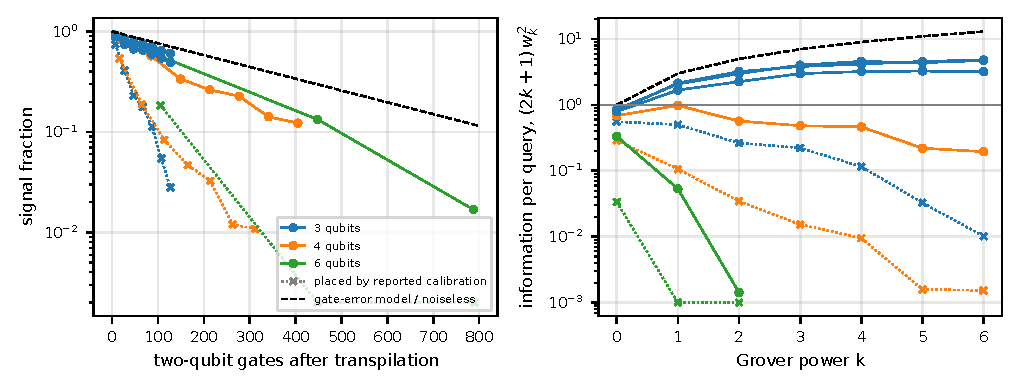
\includegraphics[width=\linewidth]{figures/hardware_depth.pdf}
\caption{Left: signal fraction against the number of two-qubit gates in the
transpiled circuit, for every register and placement; solid lines are
screened qubits, dotted lines the placement by published calibration; the
dashed line is $(1-\varepsilon)^{N}$ at the published median error
$\varepsilon = 2.7\times10^{-3}$. Right: the bound
$\Gamma_k = (2k+1)\,w_k^2$ on the information per oracle query, in units of
an ideal unamplified shot; the dashed line is the noiseless value $2k+1$,
the horizontal line marks break-even, and values below $10^{-3}$ are drawn
at $10^{-3}$.}
\label{fig:hw-depth}
\end{figure}

On screened qubits the picture changes
(Table~\ref{tab:hw-mlae}, Figure~\ref{fig:hw-depth}). The 3-qubit Grover
iterate retains $f_Q = 0.905$--$0.924$ of its contrast on three disjoint
qubit sets, and half of the signal is still present after six iterates (127
CZ gates). The 4-qubit iterate (64 CZ) retains $0.58$. The 6-qubit pricing
circuit keeps $58\%$ of its signal after state preparation alone (101 CZ),
$13\%$ after one Grover iterate (448 CZ) and $2\%$ after two.

Whether amplification pays is a separate question. Under the depolarising
contrast model, $P_k = \tfrac12 + F_k\,(\sin^2((2k+1)\theta) - \tfrac12)$,
one shot at power $k$ carries the Fisher information
\begin{equation}
I_k(\theta) = \frac{4\,(2k+1)^2 F_k^2 \sin^2 x}{1 - F_k^2\cos^2 x}
\;\le\; 4\,(2k+1)^2 F_k^2, \qquad x = 2(2k+1)\theta ,
\end{equation}
about $\theta$. An ideal unamplified shot, that is, one noiseless Bernoulli
draw of the amplitude, carries exactly $4$ and costs one oracle query; a
shot at power $k$ costs $2k+1$. The information per query, in units of an
ideal unamplified shot, is therefore at most
\begin{equation}
\Gamma_k = (2k+1)\,F_k^2 ,
\end{equation}
which is $2k+1$ without noise. If $\Gamma_k \le 1$ at every power, no
schedule on those qubits can use fewer queries than unamplified sampling on
an ideal device, whatever the amplitude. $\Gamma_k > 1$ is necessary for a
gain, not sufficient: the bound is attained only for favourable $\theta$,
and direct classical sampling of a payoff has a smaller variance than a
Bernoulli draw of its amplitude. Taking $w_k$ for $F_k$, which is exact for
global depolarising noise, $\Gamma$ reaches $3.3$, $4.7$ and $4.8$ at
$k = 5$--$6$ on the three screened 3-qubit sets, where an ideal device would
give $11$--$13$. On the screened 4-qubit set it peaks at $0.98$ (95\% CI
$[0.90, 1.06]$) at $k=1$ and stays below $0.6$ beyond. On the 6-qubit
pricing register it is $0.33$ at $k=0$ and $0.05$ at $k=1$: every Grover
iterate \emph{costs} information, even on screened qubits. On the qubits
placed by the published calibration it never exceeds $0.56$. $\Gamma$ was
defined after the data were seen; it is a description, not a pre-registered
test. Round~5 (Section~\ref{sec:res-hw5}) is that test. This is the
measured form of the resource argument of
Section~\ref{sec:res-mc}.

Three further results.
\begin{enumerate}
  \item \emph{Gate counts overstate what survives.} The slope of $\ln w$
        against the two-qubit gate count gives an effective error of
        $0.34$--$0.57\%$ per two-qubit gate on screened qubits and
        $1.9$--$2.6\%$ on the unscreened ones, against a published median CZ
        error of $0.27\%$. The probability that no CZ gate fails, computed
        from published per-gate errors, exceeds the measured signal fraction
        everywhere: $0.71$--$0.82$ against $0.50$--$0.61$ at 127 gates,
        $0.31$ against $0.13$ at 448, $0.13$ against $0.02$ at 788.
        $P_{\mathrm{ok}}$ is an optimistic planning figure, not a bound.
  \item \emph{A noise-aware likelihood recovers the amplitude at 3 qubits.}
        The platform's estimator assumes a noiseless likelihood. On the
        screened 3-qubit sets it returned amplitudes $8$--$11\%$ too high
        (true value $0.1413$). Fitting $\theta$ together with the two
        contrast parameters~\cite{tanaka2021} gave $0.1416$, $0.1401$ and
        $0.1414$, within $1\%$, and $0.1423$ even on the unscreened set. On
        the 4-qubit register it was $8\%$ low on the screened set and
        $72\%$ low on the unscreened one. The model is nevertheless
        rejected by its own goodness-of-fit test on five of the six fitted
        sets ($p < 0.01$): the contrast decays towards $0.42$--$0.49$, not
        $1/2$. We report these estimates as exploratory.
  \item \emph{A published calibration is not a measurement.} The same
        3-qubit circuits on the same device, twelve minutes apart, kept
        $3\%$ or $50$--$61\%$ of their signal at $k=6$ according to how the
        qubits were chosen. Published readout errors were wrong in both
        directions: qubit 54, published at $P(\text{read }0\,|\,1) = 0.6\%$,
        measured $8.0\%$; qubit 44, published at $7.1\%$, measured $0.95\%$
        and served in a screened set. Across the
        device, published and measured mean assignment errors agree in the
        median ($1.7\%$ and $1.7\%$) and correlate at $0.76$, but 17 of 156
        qubits were more than three times worse than published.
\end{enumerate}

\subsubsection{Round 2C: can sample-based diagonalization tell device from noise?}

We retrieved the raw counts of the three round-1 SqDRIFT jobs and ran three
analyses on each: SQD on the device counts with five SQD seeds; SQD on the
same number of bitstrings in which every bit is drawn independently from the
device's own single-qubit marginal (which keeps each qubit's bias and
removes all correlations); and SQD on uniformly random bits; five draws each
(Table~\ref{tab:hw-sqd}).

\begin{table}[H]
\centering\footnotesize\setlength{\tabcolsep}{4pt}
\begin{tabular}{lrcccccc}
\toprule
 & & Valid & HF & $P(1)$ on HF-occupied & \multicolumn{3}{c}{SQD $|$error$|$ (mHa)} \\
Setting & Shots & strings & strings & / empty qubits & Device & Shuffled & Uniform \\
\midrule
N$_2$ eq., 25 & 5\,000 & 1.38\% & 0 & 0.532 / 0.449 & $0.156 \pm 0.395$ & $0.024 \pm 0.022$ & $0.107 \pm 0.196$ \\
N$_2$ 1.8\,\AA, 25 & 5\,000 & 1.86\% & 0 & 0.541 / 0.439 & $0.015 \pm 0.022$ & $0.033 \pm 0.047$ & $0.021 \pm 0.044$ \\
N$_2$ 1.8\,\AA, 100 & 20\,000 & 1.97\% & 3 & 0.555 / 0.431 & $0.011 \pm 0.015$ & $0.034 \pm 0.050$ & $0.006 \pm 0.012$ \\
\bottomrule
\end{tabular}
\caption{SqDRIFT on \texttt{ibm\_marrakesh}, from the raw counts of round 1.
Valid strings have the right number of $\alpha$ and $\beta$ electrons
(uniform bits: 1.37\%); HF strings equal the Hartree--Fock determinant
(uniform expectation in 20\,000 shots: 0.02). SQD errors: mean $\pm$ 95\%
interval over five seeds or draws; coverage is 62--78\% in every cell.}
\label{tab:hw-sqd}
\end{table}

The device output is not uniform noise. Qubits that are occupied in the
Hartree--Fock state read 1 with probability $0.53$--$0.56$, empty ones with
$0.43$--$0.45$ (Mann--Whitney $p \le 3\times10^{-4}$ in each job); the
fraction of valid strings exceeds the uniform rate in the two stretched-N$_2$
jobs ($p = 0.005$ and $10^{-11}$) though not at equilibrium ($p = 0.95$);
and three exact Hartree--Fock strings appear in 20\,000 shots where uniform
bits would give $0.02$ ($p = 10^{-6}$). The circuits conserve particle
number, so an ideal device would return 100\% valid strings; $1.4$--$2.0\%$
is a faint, real memory of the initial state.

SQD cannot use it. The three kinds of input give the same energies: device
against shuffled, Mann--Whitney $p = 1.0$, $0.69$, $0.68$; device against
uniform, $p = 1.0$, $0.84$, $0.21$. All means are below $0.2$\,mHa, because
configuration recovery turns 5\,000--20\,000 near-random strings into a
subspace covering 62--78\% of the FCI space, where diagonalization is close
to exact whatever the input. The sub-0.1\,mHa hardware energies of round 1
were produced by the classical post-processing. At 20 qubits and these shot
counts the experiment cannot detect sampler quality on hardware; it needs
active spaces where the shot budget is far below the FCI dimension
(round~7, Section~\ref{sec:res-hw7}).

\subsubsection{Round 3: portfolio QAOA with transferred angles}
\label{sec:res-hw3}

Section~\ref{sec:res-portfolio2} left one portfolio method that returns
better selections than chance on a simulator. On 17~November 2026 we sampled
its trained circuits on the device (E22). For each of the 30 instances of
E21 the product's circuit, its QAOA ansatz of depth 2 with measurements, was
transpiled once with free angles and bound seven ways: with the trained
angles of the five E21 seeds, and with two null bindings whose ideal output
is exactly uniform (every $\gamma = 0$; every $\beta = 0$). On this device
the angles enter as virtual $Z$ rotations, so the seven bindings run one
physical gate sequence. The 150 trained angle sets were regenerated by
running the product's simulator path again and equal their E21 records, and
the exact state of every bound circuit equals the recorded one to
$2\times10^{-16}$. Sampler settings are those of the product's hardware path
(optimisation level 3, XY4 dynamical decoupling, gate twirling). The
analysis plan was committed before the first job and amended once, before
any device data existed: to spare the account's yearly allowance, the shots
at 8 and 12 assets were reduced from 10\,000 to 4\,000 per binding and the
secondary hypothesis was restricted to 16 assets. Six jobs, $1.26$ million
shots, 400\,s of QPU time; no run was excluded and no job was repeated.

Three things differ from what the product does on hardware, and they bound
what this round shows. The angles were trained on the simulator and
transferred; the product trains on the device, which this round does not
test (round~6 does, at 8 assets). The transpiler kept the best of eight seeds by two-qubit gate count;
the product makes one pass. And the primary outcome applies the product's
rule to batches of 200 shots, the sample size of the simulator path, cut
from one run of a binding after a seeded permutation, which assumes that the
device's distribution is stable over a job. This round carries the first of
the three controls named at the end of this section, in the form of the two
null bindings, and not the second: no readout calibration was taken in the
session, and the published calibration data were four days old.

\begin{table}[H]
\centering\footnotesize\setlength{\tabcolsep}{1.8pt}
\begin{tabular}{rrrrrrrcclrrl}
\toprule
 & & & \multicolumn{4}{c}{Optimum from 200 shots (\%)} & \multicolumn{3}{c}{Gap $g$ of the returned selection} & \multicolumn{2}{c}{Ratio $r$} & \\
$n$ & CZ & $P_{\mathrm{ok}}$ & device & null & unif. & sim. & device & null & $p$ & device & exact & Retained \\
\midrule
8 & 213 & 0.68 & 98.5 & 52.2 & 54.3 & 100 & $0.001 \pm 0.001$ & $0.029 \pm 0.005$ & 0.0020 & 0.39 & 0.63 & 0.386 [0.362, 0.421] \\
12 & 465 & 0.37 & 45.7 & 5.0 & 4.8 & 86 & $0.025 \pm 0.010$ & $0.124 \pm 0.026$ & 0.0020 & 0.30 & 0.65 & 0.134 [0.122, 0.159] \\
16 & 827 & 0.19 & 1.8 & 0.5 & 0.3 & 78 & $0.126 \pm 0.027$ & $0.202 \pm 0.029$ & 0.0020 & 0.15 & 0.73 & 0.004 [0.002, 0.009] \\
\bottomrule
\end{tabular}
\caption{Portfolio QAOA with simulator-trained angles on
\texttt{ibm\_marrakesh}, 17 November 2026: 10 instances per size, five
trained bindings and two null bindings each. CZ: two-qubit gates of the
transpiled circuit; $P_{\mathrm{ok}}$: probability of no two-qubit error
from the device's published gate errors. ``Optimum from 200 shots'': share
of 200-shot batches whose cheapest sample is an exact optimum, for the
trained bindings on the device, for the null bindings on the device, for
exact uniform sampling, and for the same runs on the simulator (E21). Gap:
means with 95\% intervals over 10 instances; $p$: Wilcoxon signed-rank test,
unadjusted, threshold $0.017$. Ratio: approximation ratio of the device
samples and of the exact state. Retained: share of the exact state's excess
probability of the optimum over its uniform value that the device keeps,
with a bootstrap interval over instances.}
\label{tab:hw-portfolio}
\end{table}

The pre-stated primary hypothesis holds at every size
(Table~\ref{tab:hw-portfolio}): the selection the rule returns from 200
device shots is closer to the optimum for the trained angles than for the
nulls on 10 of 10 instances ($p = 0.0020$ each; three comparisons). How much
of the simulator's result is left depends on the size. At 8 assets a batch
returns an exact optimum in $98.5\%$ of cases, against $52\%$ for the nulls
and $100\%$ on the simulator. At 12 assets it is $46\%$ against $5\%$ and
$86\%$. At 16 assets it is $1.8\%$ against $0.5\%$ and $78\%$: the returned
selection is still better than the null's, because the device's samples
remain shifted towards low cost, but from 200 shots the method no longer
finds the optimum.

The device distribution says the same without a selection rule. An optimum
has probability $3.3\%$, $0.34\%$ and $0.009\%$ in the device samples,
against $8.1\%$, $2.4\%$ and $1.5\%$ in the exact state: of the excess over
the uniform value the device keeps $39\%$, $13\%$ and $0.4\%$. At 16 assets
that is 46 optimal shots among 500\,000, where uniform sampling gives $7.6$
and the exact state about $7\,500$. If a circuit with at least one two-qubit
error returned uniform bits and one without returned the exact state, the
retained share would equal $P_{\mathrm{ok}}$; it is lower by factors of
$1.8$, $2.8$ and $42$. That product leaves out single-qubit gates, readout
and idling over a depth of 395 to 836; which of them accounts for the rest
we did not measure. The null bindings behave as uniform bits: their samples
have an approximation ratio of $0.000$, $0.002$ and $0.005$, not
distinguishable from zero ($p = 0.85$, $0.43$, $0.85$), they contain 306, 20
and 5 optimal shots where uniform sampling predicts 312.5, 19.5 and 3.1, and
the two kinds of null do not differ ($p = 0.084$, $0.32$, $0.77$). The same
gates without trained angles return what chance returns, so the effect is in
the angles.

The secondary hypothesis concerns the sample size of the product's hardware
path, 10\,000 shots, at 16 assets. There the trained bindings returned an
optimum in 28 of 50 cases and the nulls in 4 of 20, where exact uniform
sampling predicts $14\%$; the gap is $0.012$ against $0.030$, lower on 10 of
10 instances ($p = 0.0020$; one comparison, threshold $0.05$). At 8 and 12
assets, with 4\,000 shots, the trained bindings returned an optimum in 50 of
50 cases each and the nulls in 20 of 20 and 11 of 20; uniform sampling
returns one with probability $1.00$ and $0.62$. At 8 assets a sample of
that size, and so the 10\,000 shots of the hardware path, makes the circuit
irrelevant to the result. The exact
reference the product attaches agreed with the scoring here for all 210
bindings.

\subsubsection{Round 4: round 2A on a second device}
\label{sec:res-hw4}

Round~2A is one job on one device. On 20~November 2026 we ran its three
bindings again on \texttt{ibm\_kingston}, a second processor of the same
type (E26). Nothing of round~2A was changed: the instance, the circuit, the
angles, 40\,000 shots per binding, the sampler settings, and a readout
calibration in the same job. The plan was committed before the job. It
names the test of round~2A as the only criterion (one-sided Fisher exact
test of the constraint-satisfying samples against the pooled nulls,
$\alpha = 0.01$), declares every comparison between the two devices
descriptive, and states the rule that chose the device: of the account's
two other processors, the operational one with fewer pending jobs. The
circuit was transpiled anew for that device (214 CZ gates, depth 236). One
job, 128\,000 shots, 37\,s of QPU time; no job was repeated.

\begin{table}[H]
\centering\footnotesize\setlength{\tabcolsep}{5pt}
\begin{tabular}{lccccc}
\toprule
 & Ratio $r$ & Constraint-satisfying & Lowest 0.1\% & Ground level & True optimum \\
\midrule
Device, $(\gamma^\ast,\beta^\ast)$ & $0.506 \pm 0.003$ & 1.118\% [1.02, 1.23] & 1.91\% & 9 shots & 6 shots \\
Device, null $\beta = 0$ & $-0.030 \pm 0.005$ & 0.068\% [0.04, 0.10] & 0.063\% & 1 shot & 0 \\
Device, null $\gamma = 0$ & $-0.018 \pm 0.005$ & 0.075\% [0.05, 0.11] & 0.093\% & 0 & 0 \\
\bottomrule
\end{tabular}
\caption{The three bindings of Table~\ref{tab:hw-qaoa} on
\texttt{ibm\_kingston}, 40\,000 shots per row. The noiseless and the uniform
row of that table apply unchanged; intervals as there.}
\label{tab:hw-qaoa-kingston}
\end{table}

The test rejects again (Table~\ref{tab:hw-qaoa-kingston}): 447
constraint-satisfying samples against 57 in the 80\,000 null shots, sixteen
times the null rate ($p = 1\times10^{-148}$). The two nulls agree with each
other ($p = 0.79$) and with the uniform rate ($p = 0.45$); their mean energy again
differs from that of uniform sampling, here in the other direction
($r = -0.03$ and $-0.02$). Net of the nulls, the device retained 81\% of the
ideal approximation ratio and 40\% (95\% CI 36--44\%) of the ideal excess of
constraint-satisfying samples, against 63\% and 20\% in round~2A, and it
returned 447 such samples where \texttt{ibm\_marrakesh} had returned 244, a
ratio of $1.8$ (95\% interval $1.6$--$2.1$). These comparisons are
descriptive, as the plan declared: the two runs differ in device, day,
placement and age of the calibration data, and one job on each cannot
separate them.

The two figures we gave for scale do not account for the difference. From
the device's reported gate errors the probability that none of the 214 CZ
gates fails is $0.71$, and from the calibration in the job the probability
that all 18 bits are read correctly is $0.62$. Their product is $0.44$,
against $0.45$ in round~2A, where the device kept half as much of the
excess. The placement again rested on old data. The device's calibration
record, dated 44~hours before the job, gave one of the 18 qubits a readout
error of $1.0\%$; in the job that qubit read~1 in 1\,143 of 4\,000 shots
prepared in~0 and read~0 in 644 of 4\,000 shots prepared in~1. On the other
17 qubits the mean error was $1.3\%$ measured against $1.2\%$ reported. The
run replicates the result of round~2A on a second device of the same type,
for the same instance and angles. It says nothing about other instances,
other processor types or training on the device.

\subsubsection{Round 5: amplitude estimation against ideal sampling at equal queries}
\label{sec:res-hw5}

Round~2B left a bound and not a test: on three screened 3-qubit sets a
query could carry up to $3.3$--$4.8$ times the information of an ideal
unamplified shot, and $\Gamma$ was defined after the data were seen. On
20~November 2026 we ran the test on \texttt{ibm\_marrakesh}, with its
criterion fixed in advance (E27). A readout screen of all 156 qubits
rejected 75 by the thresholds of round~2B. The main job started
1.3~minutes after the screen had finished. It ran the 3-qubit register on
three disjoint sets of accepted qubits at Grover powers $k = 0$ to $8$, with
a readout calibration of each set. One estimate uses 50 shots at each power
from 0 to 6, which is 2\,450 oracle queries, and maximises the likelihood of
the contrast model of round~2B over the amplitude and two contrast
parameters, with the readout errors of the job's calibration. Every set
gave 200 estimates from disjoint blocks of shots.

The criterion compares them with ideal unamplified sampling at the same
2\,450 queries, that is, with 2\,450 noiseless Bernoulli draws. The estimate
from those draws has the standard error $t = 0.0070$ and lies within $t$ of
the amplitude $a = 0.1413$ with probability $q_0 = 0.690$ (exact). An
estimate of amplitude estimation within $t$ of the amplitude counts as a
hit, and the hypothesis that hits are more frequent than $q_0$ is tested by
a one-sided exact binomial test at $\alpha = 0.01$, which needs 441 hits of
600. Two earlier forms of the criterion were discarded before any device
data existed, after simulations had shown that one rejects without
amplification and that the other does not keep its error rate. One screen
and one main job, 549\,160 shots, 156\,s of QPU time; no job was repeated.

\begin{table}[H]
\centering\footnotesize\setlength{\tabcolsep}{4pt}
\begin{tabular}{lcccccc}
\toprule
Qubits & $f_Q$ & $\max_k \Gamma_k$ & Hits & Bias & RMSE & $\rho$ [95\% interval] \\
\midrule
(107, 97, 106) & 0.871 & 2.7 at $k=6$ & 148 of 200 & $-0.0015$ & 0.0062 & 0.77 [0.63, 1.00] \\
(31, 32, 18) & 0.822 & 2.2 at $k=4$ & 123 of 200 & $+0.0006$ & 0.0081 & 1.32 [1.09, 1.61] \\
(65, 66, 77) & 0.861 & 3.0 at $k=4$ & 148 of 200 & $+0.0002$ & 0.0062 & 0.77 [0.63, 0.96] \\
\midrule
All three sets & & & 419 of 600 & $-0.0003$ & 0.0069 & 0.95 [0.85, 1.08] \\
Ideal unamplified sampling & & & 69.0\% & 0 & 0.0070 & 1 \\
\bottomrule
\end{tabular}
\caption{Amplitude estimation with 2\,450 oracle queries per estimate on
three screened 3-qubit sets of \texttt{ibm\_marrakesh}, 200 estimates per
set. $f_Q$ and $\Gamma_k$ as in Table~\ref{tab:hw-mlae}, from all shots of
the job. Hits: estimates within $t = 0.0070$ of the amplitude $0.1413$.
$\rho$: mean squared error relative to that of ideal unamplified sampling
with the same number of queries, with a bootstrap (BCa) interval over the
estimates.}
\label{tab:hw-ae}
\end{table}

The hypothesis is not confirmed (Table~\ref{tab:hw-ae}): 419 of the 600
estimates are hits, a rate of $0.698$ (95\% CI $0.660$--$0.735$) against
$0.690$ ($p = 0.35$). The estimates have a root-mean-square error of
$0.0069$ where ideal sampling has $0.0070$, a mean squared error of $0.95$
times the ideal one (95\% interval $0.85$--$1.08$), and no bias that the
data show ($-0.0003$, interval $-0.0008$ to $+0.0003$). At equal queries,
amplitude estimation on these qubits did what an ideal classical sampler
does, and not more. The sets differ: two have a mean squared error of
$0.77$ times the ideal one and the third $1.32$ times. Their intervals
describe single sets; the criterion pools the sets.

The probe in the same job shows why the bound of round~2B was not reached.
The contrast kept per Grover iterate was $0.87$, $0.82$ and $0.86$, against
$0.905$--$0.924$ on the three sets of round~2B, which were other qubits of
the same device on 17~November, and $\Gamma$ peaked at $2.7$, $2.2$ and
$3.0$. The screen selects qubits by their readout and does not measure
their gates. For the tested schedule the bound allowed $2.5$, $1.8$ and
$2.5$ times the information of an ideal shot per query, and the estimates
realised $1.3$, $0.76$ and $1.3$: $\Gamma > 1$ is necessary for a gain and
was not sufficient here. Five other schedules, with 20 estimates per set,
had root-mean-square errors from $0.0087$ at a largest power of 2 to
$0.0067$ at 8; none of their intervals lies below the ideal value.

Unamplified sampling on the same qubits, 2\,450 shots at $k = 0$ with the
same readout correction, was biased by $+0.036$, a quarter of the amplitude
(root-mean-square error $0.037$). The state preparation alone kept a
contrast of $0.87$--$0.91$, and a sampler cannot tell lost contrast from
amplitude. The likelihood of amplitude estimation fits the contrast, and
its pooled estimates showed no bias on a device on which direct sampling
was biased. That comparison does not isolate amplification. The test covers
one amplitude, known in advance, on one 3-qubit register in one job, and
its 600 estimates share three qubit sets and their calibrations. Its
currency is queries, not cost: an estimate took 350 shots of circuits with
7 to 127 CZ gates, and the sampler it is compared with is a computed
reference, not a device.

\subsubsection{Round 6: portfolio QAOA trained on the device}
\label{sec:res-hw6}

Round~3 transferred its angles from the simulator. The product's hardware
path trains them on the device with an Estimator, and it had never been
run. On 21~November 2026 we ran it (E28) in three phases, with the plan
committed before the first job.

\emph{The path as shipped.} First the product's own call, unchanged, for
the first 8-asset instance of E21 with the 5 iterations to which the
gateway caps a default hardware request. The device it chose, the one the
service reported as least busy, was \texttt{ibm\_fez}. The call ran end to
end: six Estimator jobs that each ask for 1\,000 shots (the service ran
1\,024 in 16 twirled variants),
11\,s of QPU time each, and one sampler job of 10\,000 shots (5\,s); 71\,s
of QPU time and 3.6 minutes in all. There are six jobs because SciPy raises
a COBYLA limit of 5 to 6 for four parameters. Six values are the start, one
step along each of the four angles and one further point; the call returns
the best of them. Its selection was an exact optimum, which 10\,000 uniform
samples of 256 selections contain as well.

\emph{Training.} The ten 8-asset instances of E21 and round~3 were then
trained on that device with the settings of the product's path: COBYLA from
the product's initial angles with its tolerance and its default of 12
objective values, every value an Estimator estimate with the options of
the product's call (1\,000 shots asked, XY4 decoupling, gate twirling), on circuits from one transpiler pass (222
CZ gates, depth 430, the same eight qubits for all instances). The ten
instances shared one job per step; a replay of the optimiser on the
recorded values gives each instance its next point. After the first phase
and before any training job the plan was amended once: its budget rule had
been written before the cost of an Estimator job was known. The amendment
raised the budget and fixed what would be dropped if a step proved
expensive; it depends on QPU seconds only. The first step used 14\,s, and
the plan ran as first registered. A pause of 35 minutes lies between the
first step and the other eleven; 43 minutes passed from the first step to
the evaluation.

\emph{Evaluation.} One sampler job bound every instance's circuit ten ways
with 2\,000 shots each: the initial angles (S), the angles a capped request
returns from the first six values (D5), the angles after twelve values
(D12), the five transferred angle sets of round~3 (T) and its two nulls,
with a readout calibration in the same job (mean error $0.8\%$). The
pre-stated primary test compares the approximation ratio of D12 with the
mean over T (two-sided exact Wilcoxon signed-rank test over the ten
instances, $\alpha = 0.01$), the secondary one D12 with S (one-sided,
unadjusted). 20 jobs, 310\,s of QPU time; no job was repeated.

\begin{table}[H]
\centering\footnotesize\setlength{\tabcolsep}{5pt}
\begin{tabular}{lcccc}
\toprule
Angles & $r$, device & $r$, exact & Optimum (exact) & In 200 shots \\
\midrule
Start (S) & $0.162 \pm 0.040$ & 0.284 & 0.92\% (1.65\%) & 86\% \\
After six values (D5) & $0.254 \pm 0.041$ & 0.452 & 1.72\% (4.17\%) & 90\% \\
After twelve values (D12) & $0.345 \pm 0.033$ & 0.623 & 2.68\% (7.18\%) & 100\% \\
Transferred (T) & $0.349 \pm 0.044$ & 0.631 & 2.93\% (8.05\%) & 98.8\% \\
Nulls & $0.003 \pm 0.009$ & 0 & 0.36\% (0.39\%) & 52\% \\
\bottomrule
\end{tabular}
\caption{Portfolio QAOA at 8 assets on \texttt{ibm\_fez}, 21 November 2026:
means over the ten instances with 95\% intervals over instances; 2\,000
shots per binding. $r$: approximation ratio; exact: the same angles on an
ideal device. Optimum: probability of an exact optimum in the device's
samples and, in brackets, on an ideal device. In 200 shots:
share of the batches of 200 shots that contain an exact optimum; uniform
sampling gives 54\%.}
\label{tab:hw-train}
\end{table}

Training on the device worked, and it ended where transfer ends
(Table~\ref{tab:hw-train}). D12 has the larger ratio on 4 instances and T
on 6; the median difference is $-0.011$ (range $-0.082$ to $+0.135$,
$p = 0.56$): no difference is shown. D12 is better than its start on 10 of
10 instances ($p = 0.00098$, median $+0.18$), and the six values of a
capped request improve on the start on 9 of 10. The device-trained angles
are not better on the device than their exact quality predicts: on an ideal
device they give $r = 0.62$ against $0.63$ for the transferred ones, and
the device keeps $0.56$ and $0.55$ of those ratios. Round~3, on another
device and with the best of eight transpiler seeds, kept $0.62$.

The cost is the other result. An objective value took 11\,s of QPU time for
one instance and 14\,s for ten in one job. A capped default run used
71\,s for one 8-asset instance, and the six values of such a run took the
ratio half of the way from the start to the transferred level; twelve values in separate jobs, as the
product submits them, would use about 140\,s per instance. Transferred
angles use none of it and were as good. The round covers 8 assets, twelve
values, one session and one device; the arms are compared at equal
evaluation shots, and the device-trained arm used the shots of twelve
Estimator values per instance before them.

\subsubsection{Round 7: sample-based diagonalization on a 24-qubit active space}
\label{sec:res-hw7}

Round~2C ended with what the experiment needs: an active space far larger
than the shot budget. On 21~November 2026 we ran one (E29): N$_2$ at
1.8\,\AA{} in cc-pVDZ with ten electrons in twelve orbitals, 24 qubits and
627\,264 determinants, through the product's pipeline unchanged: its
circuit builder, 100 shots per circuit, and its diagonalization with
configuration recovery at the default settings.

\emph{Design phase.} A simulator pilot on four groups of 50 circuits came
first, and the plan reports what it showed. From noiseless samples the
pipeline's error was 65.6\,mHa with a subspace of 1.4\% of the space; from
uniformly random bits it was 4.4\,mHa with 35\%. Noiseless samples gave a
smaller error than strings drawn from their own single-qubit marginals in
4 of 4 groups at this bond length and in 2 of 4 at the equilibrium one,
which is why the stretched bond was chosen. The largest error of
the pipeline on circuit or device samples in the stored results of the
earlier experiments is 24\,mHa.

\emph{Plan.} Ten groups of 50 circuits with fixed seeds, 5\,000 samples per
group, on \texttt{ibm\_marrakesh} in three jobs, each with a readout
calibration. Every circuit was transpiled by itself with a fixed seed: 403
to 1\,650 two-qubit gates (median 872.5) at depth 614 to 3\,861. By the error
rates the device reported, a circuit runs without a two-qubit error with
probability $0.13$ in the median ($0.02$ to $0.47$). Each group went
through the product's diagonalization five times: with the device's samples;
with the same number of strings in which every bit is drawn independently
from the device's marginal for that qubit, as in round~2C; with uniform
bits; with noiseless samples of the same circuits from the simulator; and
with strings drawn from the marginals of those. The pre-stated primary test
asks whether the pipeline returns a smaller error from the device's samples
than from their marginals (one-sided exact Wilcoxon signed-rank test over
the ten groups, $\alpha = 0.01$). Two secondary tests, unadjusted, compare
the device's samples with the noiseless ones (one-sided) and with uniform
bits (two-sided). The plan states that an error below another's can come
from a larger subspace and reports the dimension with every error. Three
jobs, 37\,s of QPU time; no job was repeated.

\begin{table}[H]
\centering\footnotesize\setlength{\tabcolsep}{5pt}
\begin{tabular}{lccccc}
\toprule
Input & $|$error$|$ (mHa) & Subspace & Selected CI & Valid & HF \\
\midrule
Device samples & $6.3$ ($4.1$--$12.3$) & 27.1\% & 0.58 & 3.77\% & 0 \\
Device marginals & $7.5$ ($4.5$--$12.4$) & 26.9\% & 0.59 & 4.04\% & 0 \\
Uniform bits & $5.9$ ($3.5$--$11.9$) & 35.3\% & 0.28 & 3.69\% & 0 \\
Noiseless samples & $64.1$ ($42.9$--$98.5$) & 1.19\% & 17.0 & 100\% & 59.8\% \\
Noiseless marginals & $101.5$ ($99.8$--$103.5$) & 0.34\% & 29.6 & 30.9\% & 23.7\% \\
\bottomrule
\end{tabular}
\caption{SqDRIFT for N$_2$ in a 24-qubit active space on
\texttt{ibm\_marrakesh}, 21 November 2026: means over ten groups of 5\,000
samples, with the range over groups, at the product's default settings
(three batches of 300 samples, at most five recovery iterations). Subspace:
mean dimension as a share of the 627\,264 determinants. Selected CI: error
in mHa of a classical selected CI of that dimension on the same problem,
interpolated. Valid: samples with five $\alpha$ and five $\beta$ electrons
(uniform bits: 3.74\% expected). HF: samples equal to the Hartree--Fock
determinant.}
\label{tab:hw-sqd24}
\end{table}

The primary test is not confirmed (Table~\ref{tab:hw-sqd24}). The error from
the device's samples is smaller than from their marginals in 7 groups and
larger in 3 (median difference $-0.65$\,mHa, range $-7.1$ to $+1.5$,
$p = 0.14$): the pipeline's energy does not tell the device's samples from
strings that keep only each qubit's bias. Nor does it tell them from uniform
bits (smaller in 2 of 10 groups, $p = 0.375$). On the simulator the same
comparison separates: noiseless samples beat their own marginals in 10 of 10
groups ($p = 0.00098$; four of the ten had been seen in the design phase).

The device output is close to noise. Of its 50\,000 samples, 1\,886
($3.77\%$) have the right electron numbers, where uniform bits give
$3.74\%$, and none equals the Hartree--Fock determinant, which makes up
$59.8\%$ of the noiseless samples. What survives is a bias: the device's
marginals differ from $1/2$ by $0.06$ on average, and from the noiseless
marginals by $0.38$. The readout calibrations found a mean error of
$2.6$--$3.6\%$ over the 127 to 135 qubits the circuits of a job used; in
every job at least one of them read one of its two states wrongly about
half of the time.

The secondary comparison goes the way one would not wish. The device's
samples give a ten times smaller error than noiseless samples of the same
circuits, $6.3$ against $64.1$\,mHa, in 10 of 10 groups ($p = 0.00098$). The
reason is the size of the subspace and not the quality of the samples.
Noiseless samples concentrate: a group of 5\,000 holds about 250 distinct
configurations, and recovery builds $1.2\%$ of the space from them. Nearly
all strings of the device are distinct, and recovery builds $27\%$ from
them and $35\%$ from uniform bits. At equal dimension a classical selected
CI has about 11 times less error than the pipeline has from device samples
and about 4 times less than it has from noiseless ones. A reader of the
product's result alone would rank the three inputs in the wrong order:
uniform bits first, device samples second, the noiseless circuit last.

At 20 qubits round~2C could not detect sampler quality because recovery
filled most of the space. Here it fills $37\%$ at most, the error no
longer vanishes, and the finding sharpens: on this problem the reported
energy rewards the number of distinct configurations a sampler delivers,
and noise delivers them. The round covers one molecule, one active space,
one geometry, one device and the product's default settings.

\subsubsection{Round 8: a placement chosen from old calibration data}
\label{sec:res-hw8}

Rounds~2 to~4 were placed with calibration data that were days old, and
the largest single effect in round~2B was a choice of qubits. Round~8
isolates that choice (E30). On 26~November 2026 one job on
\texttt{ibm\_marrakesh} ran the circuit of round~2A on three placements
that differ only in the age of the calibration data that chose them.

The plan was committed before the first snapshot of the device's error
data was stored. The circuit, depth-1 QAOA on 18 qubits at its
exact-optimal angles, is routed once on the coupling map without any error
data (optimisation level~3, eight transpiler seeds, the circuit with the
fewest two-qubit gates: 214 CZ gates, depth 239). All 284 placements of its
interaction graph on the device are enumerated. A placement is scored under
a set of error data by the product of $(1 - \text{error})$ over every gate
application and every measurement of the routed circuit, and a placement
that uses a gate or a readout whose error is missing or reported as 1 is
not eligible. The
job holds the circuit on the placement with the highest score under the
errors the device reports at submission (``fresh''), the same circuit on
the placement with the highest score under a stored snapshot of each
requested age, and a null on the fresh placement ($\beta = 0$, with a
uniform ideal output), with 40\,000 shots each and the sampler settings of
round~2. All arms apply the same gates in the same order; they differ in
the physical qubits. The outcome is the number of constraint-satisfying
samples. Each age has one test, a one-sided Fisher exact test of fresh
against stale, at a family-wise $\alpha = 0.01$ over three requested ages,
that is $0.0033$ per test.

The plan asked for ages of 6, 24 and 72 hours. The workstation that stores
the snapshots was suspended for almost five days, and on the day of the job
the stored snapshots were a few hours or about five days old. An amendment, committed
before any job was submitted and before any placement was computed from a
stored snapshot, replaced 72 by 120 hours and kept the 24-hour age as
requested and unserved, so that the threshold per test stayed the same. At
submission the device's calibration data were 32~minutes old. The two
snapshots had been read $5.0$ and $119.2$ hours earlier, each within
20~minutes of the calibration it holds, and both are inside the tolerance
of 25\% that the plan allows around a requested age. Under the data of the
submission 211 of the 284 placements were eligible, with scores from
$0.015$ to $0.248$ (median $0.095$). One job, three circuits, 160\,000
shots, 48\,s of QPU time; no job was repeated.

\begin{table}[H]
\centering\footnotesize\setlength{\tabcolsep}{3pt}
\begin{tabular}{lccccccc}
\toprule
Data that chose & Qubits & \multicolumn{2}{c}{Score under the data} & & Constraint- & Lowest & Ground, \\
the qubits & shared & of its choice & of the job & Ratio $r$ & satisfying & 0.1\% & optimum \\
\midrule
Read at submission & 18 & 0.248 & 0.248 & $0.522 \pm 0.003$ & 1.273\% [1.17, 1.39] & 2.12\% & 9, 9 \\
$5.0$\,h old & 12 & 0.374 & 0.199 & $0.502 \pm 0.003$ & 0.985\% [0.89, 1.09] & 1.64\% & 13, 6 \\
$119.2$\,h old & 9 & 0.320 & 0.114 & $0.458 \pm 0.003$ & 0.823\% [0.74, 0.92] & 1.48\% & 11, 2 \\
Null, first row's qubits & 18 & & 0.248 & $-0.002 \pm 0.005$ & 0.055\% [0.03, 0.08] & 0.080\% & 0, 1 \\
\bottomrule
\end{tabular}
\caption{Round~8 on \texttt{ibm\_marrakesh}: one routed circuit on three
placements, 40\,000 shots per row. ``Qubits shared'' counts the physical
qubits a placement has in common with the first row; the null has
$\beta = 0$. The last column gives the shots at the ground level of the QUBO
and at the true optimum. The noiseless and the
uniform row of Table~\ref{tab:hw-qaoa} apply unchanged; intervals as there.}
\label{tab:hw-stale}
\end{table}

Both tests reject (Table~\ref{tab:hw-stale}). The fresh placement returned
509 constraint-satisfying samples, the placement chosen from five-hour-old
data 394 ($p = 7\times10^{-5}$) and the one chosen from five-day-old data
329 ($p = 2\times10^{-10}$): $0.77$ (95\% interval $0.68$--$0.88$) and
$0.65$ ($0.56$--$0.74$) times the fresh rate. The null returned 22, so the
fresh placement carries a signal ($p = 2\times10^{-122}$; this check is
outside the family of tests). With 40\,000 shots per arm a test detects a
drop of 21\% of the observed fresh rate with power $0.8$.

The device's own report shows what happened. Under the snapshot that chose
it, the five-hour placement had a score of $0.374$. Under the data of the
submission it has $0.199$, below the $0.248$ of the fresh placement, with
which it shares 12 of its 18 qubits. The five-day placement fell from
$0.320$ to $0.114$ and shares 9. The scores order the three placements as
the counts do, and as the approximation ratio does, but they do not give
the size of the loss: the five-day placement has $0.46$ of the fresh score
and returned $0.65$ of the fresh rate.

The round is one job on one device on one evening, with one circuit. It
shows that on that evening calibration data five hours old cost a placement
23\% of its constraint-satisfying samples (95\% interval 12--32\%), and
five-day-old data 35\% (26--44\%). It says nothing about the 24~hours in between, which the snapshots
could not serve, about other days or about other devices. It compares the
best placement by fresh data with the best placement by old data among the
placements of one routed circuit; a transpiler that also routes by error
data is a different procedure. The three circuits ran within 49~seconds of
each other, so drift inside the job is small against the ages compared.
For scale, and descriptively: round~2A, placed by the transpiler with
readout data $3.9$~days old, had returned 244 such samples on this device,
and round~4, with a record 44~hours old, 447 on the second one. Those runs
differ from this one in day and in how the placement was chosen.

\finding{On current hardware, the metrics a pipeline reports can improve
while the quantum signal disappears, and a circuit's fate can depend more on
which qubits it lands on than on its depth. Three controls separated signal
from artefact here: a depth-matched null circuit, a calibration measured in
the session, and input shuffled within its own marginals. Round 2 carries
all three, round 3 the first. Round 4 repeated the null test of round 2 on
a second device, where it rejected again. Round 5 tested in advance whether
amplitude estimation on screened qubits beats ideal sampling at equal
queries; it was as accurate and not more. Round 6 trained the product's
portfolio circuit on the device: twelve objective values brought it to the
approximation ratio of transferred angles. Round~7 took sample-based
diagonalization to 24 qubits, where recovery cannot fill the space: the
energy did not separate device samples from their marginals or from uniform
bits, and it was ten times closer to exact from all three than from
noiseless samples, because noise enlarges the subspace. With the null, a QAOA state
trained on a simulator
kept $39\%$ of its excess probability of the optimum at 213 two-qubit gates
and $0.4\%$ at 827, and the selection read from 200 shots stayed better than
chance at both. Round~8 held one circuit fixed and varied the age of the
calibration data that chose its qubits: against the choice from data read
at submission, the choice from data five hours old returned 23\% fewer
constraint-satisfying samples and the choice from data five days old 35\%
fewer, in one job, on one evening.}

%======================================================================
\section{Discussion}
\label{sec:discussion}

\inbrief{Seven lessons that cut across the workloads. A referee changes
what can be said about a result, and it has to stand where the user stands.
The name of a method is a claim and needs a
test of the step that defines it. In every hybrid pipeline we measured,
classical components supplied most of the quality, so the quantum
contribution has to be measured by ablation at every stage up to the screen.
Circuit depth, not the number of queries, decides where amplitude estimation
pays. The calibration of a device is part of the experiment. An analog
device restricts the instances it can represent. And interfaces overclaim,
with a language model and without one, unless their statements are tested.}

\subsection{What the referee rule changes}

Five statements that the platform could make about its results do not
survive a referee: annealing ``matching the
baseline'' on facility location (the baseline is not optimal); an annealed
routing plan ``shorter than the classical one'' (it leaves more stops
unserved); SqDRIFT ``reaching chemical
accuracy'' (the subspace covers the whole space); a Rydberg mapping twice
as good as its control (the control was not tuned); and SqDRIFT on hardware
``beating simulation'' (uniform
noise does as well). In each case the first plausible number would have
been accepted without one. A referee is the
only protection we know against that, and it has to cover the experiment as
well as the product: an estimator is held to its information bound, a
control is tuned, and a referee that is named is also run
(Section~\ref{sec:audit}).

It also has to stand where the user stands. Of the four portfolio methods
(Section~\ref{sec:res-portfolio2}), one computes what its
name says and is still not better than uniform samples when the number of
assets is capped. And the one method whose selections are better than
chance, on fresh instances, on a second instance family and on hardware,
changes nothing a user sees, because the classical weighting that follows
arrives at the same portfolio without it. We found the second only because
an observation on the deployed panel was turned into an experiment on the
executor and not into an argument about the selection.

\subsection{A name is a claim}

The name of a published algorithm on a method is a claim about what the
method computes. Tests that ask whether the code runs and returns a
plausible portfolio do not check it. A referee for a named method is the
definition in the cited paper, turned into a test: the objective of
CVaR-VQE must be a
CVaR of samples, the circuit of a counterdiabatic method must contain the
counterdiabatic term, the correlators of a Pauli-correlation encoding must
be measured in their bases. The three portfolio methods named after such
sources carry tests of their defining step (63 in all). Such tests settle
what is
computed. They do not settle whether it helps, which
Section~\ref{sec:res-portfolio2} had to measure separately; and where a
source leaves a choice open, as with the time grid of BF-DCQO, the name can
still promise more than our implementation has shown.

\subsection{Where the quality comes from}

In every hybrid pipeline we measured, classical components supplied most of
the solution quality: repair and local search in facility location,
configuration recovery and diagonalization in chemistry, greedy repair in
MIS, repair and a greedy fill in mission allocation, and for portfolios
best-of-many selection, re-weighting and a swap search. This is how hybrid methods are meant to work, but it means that the
quantum contribution must be measured by ablation, not inferred from the
final answer. The ablations are informative in both directions. Held against
random strings, the noiseless SqDRIFT sampler carries real information;
held against selected CI, far less than a classical method extracts. Held
against uniform bits on hardware, none that SQD can use. Evaluated exactly,
the QAOA ansatz carries a 34- to 189-fold
enrichment of feasible assignments at its best parameters, far more than
the platform's training finds. Run
against uniform bits through their own code, two portfolio methods owe
their optima to the classical search that follows the sampling, which
reaches them from uniform samples; what their circuits contribute is
visible only before that search. For QAOA the selection is better than
chance, and the classical weighting that follows displays the same
portfolio with it as without it in 138 of 150 runs. An ablation is therefore
needed at every stage a result passes on its way to the user, including the
last. The seventh workload adds that a null has a quality of its own.
Random bitstrings through the production repair and fill are a greedy
heuristic with random starts, $0.88\%$ from the optimum where one greedy
pass is $4.1\%$ away, so a method that ``beats its null'' there beats a
classical method by less than a percentage point. Given the time the
annealed reads take, that null was not shown to be behind them, and the
exact referee was faster than both. And a sampler that was
better on the QUBO was no better once the same stages followed it
(Section~\ref{sec:res-mission}). The
ablations we added (matched nulls, shuffles, a selected-CI curve, exact
state evaluation, uniform bits through the production code, a selection
replaced by every asset) are cheap at
these sizes and should be standard.

\subsection{Depth, not queries, sets the crossover}

Amplitude estimation is the only workload with a proven query advantage, and
we reproduced it down to its Cram\'er--Rao bound. Its circuits grow linearly
with the Grover power, and the power needed for the advantage pushes
two-qubit gate counts into the thousands. The hardware probe turns this into
a measured statement: on the device we used, a query could carry three to
five times the information of an unamplified sample on a 3-qubit register on
screened qubits, where an ideal device would give eleven to thirteen; it
broke even at best on 4 qubits; and every Grover iterate lost information on
the 6-qubit register that prices the option. That was a bound. The test
fixed in advance measured what an estimator realises: on three screened
3-qubit sets, with a bound of $2.2$ to $3.0$ in that job, estimates at
equal queries were as accurate as ideal unamplified sampling and not more.
A useful
resource estimate must be attached to the run and must be calibrated against
such a probe; a product of published gate fidelities overstated the
surviving signal by up to a factor of 7.6 even on screened qubits.

The third hardware round shows the same for an optimisation circuit. With
213, 465 and 827 two-qubit gates, 39\%, 13\% and 0.4\% of the optimum's
excess probability survived, less than the published gate errors predict by
factors of 1.8, 2.8 and 42. The returned selection stayed better than that
of the null bindings at all three depths, because the cheapest of many shots
needs only a small excess; the optimum itself was in 98.5\%, 45.7\% and
1.8\% of the batches of 200 shots. The sixth round locates the loss in the
sampling and not in the training: at 8 assets, angles trained on the device
were as good as transferred ones, on the device and on an ideal one, and
both lost the same share of their ratio.

\subsection{Calibration is part of the experiment}

The largest single effect in our hardware data was not an algorithm or a
depth but a choice of qubits made with three-day-old calibration data. A
platform that submits to hardware on a user's behalf should measure the
qubits it is about to use, in the same session, and record what it found.
We treat a readout screen as part of the hardware path. Round~4, which
repeated an unscreened run, met the reason on a second device: placed with
a calibration record 44~hours old, the circuit used a qubit that was read
wrongly in 22\% of its calibration shots in the job. Round~8 measured the
cost of age alone, with the circuit and its routing held fixed: qubits
chosen from data five hours old returned 23\% fewer constraint-satisfying
samples than qubits chosen from the data of the submission, and qubits
chosen from data five days old 35\% fewer. The device's own error report,
read again at submission, ranked the three choices as the counts did. Reading
the calibration at submission and choosing the qubits then costs no QPU
time; a screen in the session costs a little and sees what the report does
not.

\subsection{Modality matters, and so does geometry}

The Rydberg results show that an analog device solves its native problem
when the mapping respects its physics, and that its geometry restricts the
instances it can represent. Unit-disk graphs with dense clusters cannot be
embedded at all, and non-unit-disk graphs need gadget
constructions~\cite{nguyen2023} that multiply atom counts. A vendor-neutral
platform must therefore route by problem structure, not by qubit count.

\subsection{Interfaces can overclaim on their own}

The most persistent source of overclaiming in a system like ours is not the
algorithms but the natural-language layer. Language models reproduce popular
descriptions of quantum computing that are false at these sizes.
Prompting reduces but does not eliminate this; a deterministic filter does,
for the answers it covers. As
language interfaces become the default entry point to quantum services, their
honesty becomes a property to test, like any other.

Interfaces without a language model can overclaim as well, and need no wrong
algorithm for it: defaults that differ between the panel and the
configuration that was measured, options that no back-end reads, a figure
of merit with no measurement behind it, a recommendation by fixed scores, a
failure answered with a plausible result. The platform's rule is that a
statement on the screen is followed back to a measurement and removed where
there is none. Tests hold it in place. Tests compare the figures that
product texts quote with
the result files of the experiments. The interface's simulator presets for
the four gate-model portfolio methods are compared with the measured table
option by option. The selector behind the recommended path of the portfolio
wizard returns the classical method and says that no measurement supports
another choice. And tests cover three ways in which a result could appear
that nobody computed: a substitute portfolio after a failed run, random
weights from a simulator path, and a failed run stored as completed. One
limit is stated where the method
is offered: a multi-period portfolio method samples its
circuit with two shots per evaluation, the settings of its unit tests. The
evaluation behind these tests was not exhaustive
(Section~\ref{sec:limitations}), and every path without a referee should
be read with reserve.

Documentation is a further copy of every claim, and it ages without
failing. A call of the programming interface is reachable only if the
service that the routing
selects for its path implements it, and a test compares the
documentation with the routing rules and the routes of both services.

%======================================================================
\section{Limitations and threats to validity}
\label{sec:limitations}

\inbrief{What the results do not show. The instances are small, seeded and
within classical reach, chosen so that exact referees exist. Apart from the
hardware rounds every quantum result is a noiseless simulation, and
annealing is simulated. Settings were tuned on the reported instances, which
favours the quantum paths. The hardware evidence is eight sessions on one
processor type. The routing referee is a heuristic, and some portfolio paths
have no referee yet. One person built the platform, ran the experiments and
checked them, and no third party has yet checked the public results.}

\paragraph{Internal validity.} Penalty weights, sweep shapes and effort
presets were tuned on the instances we report, which favours the quantum
paths. The QAOA study uses one 18-variable instance; it shows what
normalisation and training do on that instance and supports no general
statement about QAOA. Its
exact-objective values are best-of-50 local optima, hence lower bounds. The
selected-CI referee is PySCF's string-product selected CI at default
settings, not a determinant-based method; a stronger referee would widen the
gap we report. $p$-values are unadjusted for multiple comparisons.

\paragraph{Portfolio experiments.} Instances are synthetic price series from
two generators, a factor model and the product's simulated market data, at
8, 12 and 16 assets, where enumeration is exact and nothing is beyond
classical reach. E20 ran on instances that an earlier experiment had used; the
independent tests are E21 and E23, and they cover QAOA only. The budgets of
CVaR-VQE and PCE come from an exploratory grid on held-out instances. Where
a source leaves a choice open the choice is ours
(Table~\ref{tab:pf-corrected}), and we do not claim to reproduce the cited
results. BF-DCQO was measured on a local simulator; a default run of the
product submits it to the vendor's cloud simulator, which we exercised but
did not measure. All QAOA
results are for the product's start of the training; the opposite
assignment of its two ramps was not better (E25, Section~\ref{sec:res-portfolio2}), and
neither start was tuned. E24 covers one method, one instance
family and runs without a limit on the number of assets; its second test
could only have shown harm (Section~\ref{sec:res-portfolio2}). The presets
for hardware runs are cost caps; the default one was measured at 8 assets
only (Section~\ref{sec:res-hw6}), and the assistant's
run-quality tiers were not measured. The annealing methods, the Cirq
implementations, the multi-period variant and one further IBM variant of the
workload have no referee yet and should be read with reserve
(Section~\ref{sec:discussion}).

\paragraph{Mission resource allocation.} The 60 instances come from one
generator, the one behind the workspace's custom scenario. At equal numbers
of assets and tasks they have fewer allowed pairs than the built-in
scenarios (26--32 against 69 at 6 assets and 18 tasks, 35--49 against 95 at
8 and 24, 60--72 against 87 at 10 and 30), and on the scenario the workspace
opens with the null was ahead. The sampler is a classical simulated
annealer; no annealing hardware and no gate-based device was used. The
comparison with 1\,024 random bitstrings was described and not tested.
The comparison at equal time (E32) is one of this implementation on one
workstation, measured once per run while the workstation also ran a local
development cluster: the annealer is compiled code and the repair and fill
are Python, so another implementation would shift it, in either direction.
Its primary test did not reject, which does not show that the two arms are
equal, and the tests by size, which point in opposite directions, were
secondary. The 15 larger instances are described only, five per size, and
one of them has no proven optimum. Part~B is exact and small: at most 19 variables, the best angles
a search found, no noise, and the platform's circuit with a transverse-field
mixer. It says nothing about constraint-preserving mixers, about larger
instances or about a device. The model is simple: straight-line travel,
fixed task times, one asset per task and a round trip charged for every
task.

\paragraph{Hardware.} Three devices of one processor type and eight sessions;
only the first experiment of round~2 was repeated on a second device, in
one job. Round~2 was a single
night; qubit screening changed the contrast kept per 3-qubit Grover iterate
from $0.46$ to $0.91$,
which is itself a warning about what one run can show. The screened run is
post hoc: it was designed after the pre-registered run was seen, its plan
was amended once after a failed transpilation, and both versions were
committed only locally before its jobs. The information bound $\Gamma_k$
was defined after the data were seen; the test of round~5 was fixed in
advance and covers one amplitude on three qubit sets in one job. The screen measures readout only,
with all qubits read at once. The noise-aware amplitude estimates rest on a
model that the data reject on most qubit sets. QAOA angles were computed
classically in rounds~2 to~4 and~8. Round~6 ran the product's training on the
device at 8 assets only, with twelve objective values per instance in one
session; the sizes 12 and 16, longer training and requests above the
gateway's cap are untested. Round~7 is one molecule, one active space, one
geometry and the product's default settings; its errors are reported with
their subspace dimensions because the two cannot be read apart. Round~3 kept the best of eight transpiler seeds where the
product makes one pass, had no readout calibration in its session and
relied on published calibration data four days old. Round~8 is one job
with one circuit on one device on one evening: its two ages are five hours
and five days, the 24-hour age it had requested was not served, and its
amendment, though committed before any job, was written after the
snapshots that it uses had been stored. No error mitigation
beyond dynamical decoupling and twirling was used.

\paragraph{External validity.} Instances are small and seeded; they were
chosen so that exact referees exist, and none is beyond classical reach.
Results on larger, real-world instances may differ in either direction.
Apart from Section~\ref{sec:res-hw}, quantum results come from noiseless
simulators; annealing results come from simulated annealing, not annealing
hardware; the analog protocol ran on a simulator of the ideal Hamiltonian.

\paragraph{Construct validity.} Gaps are measured in the problem's own
objective; distance alone was shown to be misleading for routing. For QAOA,
``constraint-satisfying'' refers to the constraints the QUBO encodes, which
exclude capacity. The signal fraction assumes that the noise component is
uniform, which readout bias violates slightly. Correlation recovered is a
poor proxy for chemical accuracy.

\paragraph{Referees.} The routing referee remains a heuristic, so its gaps
are lower bounds on the true distance to optimal; it lost to the method
under test on three runs. The portfolio referee is exact only up to the
sizes an enumeration reaches.

\paragraph{The platform.} The evaluation of the product's texts and failure
paths (Section~\ref{sec:discussion}) walked the main views with their
default runs and read the method catalogue, the recommenders and the
documentation pages. It was not exhaustive: other scenarios and the answers
of the language model were not examined and may contain statements with no
measurement behind them;
the advisors of the workload views and the automated reviewer are
constrained by their prompts alone. The automated comparison of the
documentation with the system covers the calls it names; its other
statements were checked by hand, once. The access
layer of Section~\ref{sec:architecture} is described, not evaluated:
no security review was made, and no result in this paper rests
on it.

\paragraph{Independence.} A single person, working with AI assistants
(see Acknowledgements), built the platform, ran the experiments and checked
them; the checks used the same kind of assistant that had helped to write
the code they examine. The scripts, solver code, raw results and raw
hardware counts are public, with a pinned container, so that others can check
them; no third party has yet done so. Earlier public versions of this paper
and of its archive contain results that later checks invalidated; the
release notes of the archive list them.

%======================================================================
\section{Research agenda}
\label{sec:agenda}

\inbrief{Twelve open questions, seven of them with the experiment that would
answer them, and three runs on other hardware that follow from the designs
of this paper and have not been made.}

The study suggests open questions for both the research community and
industrial users. We list them and, where we can name it, the experiment
that would answer each.

\begin{enumerate}
  \item \textbf{Referee standards.} What counts as an acceptable classical
        referee for a given problem class and size, and how should time,
        energy and cost budgets be matched? \emph{Experiment:} a shared,
        versioned ledger of instances, exact or best-known optima, and
        referee configurations, with results from many vendors.
  \item \textbf{Attributing quality in hybrid pipelines.} Which metrics
        isolate the quantum contribution when classical repair dominates?
        \emph{Experiment:} systematic ablations (matched null circuits, raw
        versus refined, shuffled samples) across workloads and devices; for
        mission allocation, tested runs at the sizes where the exact solver
        stops being the fastest method, from about a thousand variables,
        which E32 only describes on five instances per size, and a repair
        and fill in compiled code, so that equal time is closer to equal
        work.
  \item \textbf{A selection problem the weighting step cannot solve.} When
        does a selection change the portfolio that is displayed?
        \emph{Experiment:} the arms of E24 under a binding limit of $K$
        assets, with selections scored by the objective of the weighting
        step they feed, against the best $K$-subset by enumeration and
        against classical subset heuristics; and the same arms for the
        other three methods.
  \item \textbf{Constraint handling without penalties.} Do
        constraint-preserving mixers~\cite{hadfield2019}, native analog
        constraints, or feasible-subspace encodings improve on the penalised
        one-hot encoding, and can capacity be encoded so that the QUBO
        optimum is the problem's optimum? The mission QUBO leaves the duty
        limit to repair in the same way, and a QAOA on it was better on the
        QUBO and not on the problem; whether a mixer that keeps the rules
        changes that is open.
  \item \textbf{Training variational circuits to their ansatz limit.} How far
        is a shipped training procedure from the best parameters, and which
        of exact-expectation training, multi-start and parameter
        transfer~\cite{shaydulin2023,sureshbabu2024} closes the gap at what
        cost? \emph{Experiment:} the three-arm design of
        Section~\ref{sec:res-qaoa} on many instances and problem families;
        for portfolios, training on the device at 12 and 16 assets and with
        more objective values, where round~6 covers 8 assets and twelve
        values, other starts of the training than the two of E25,
        and the capped CVaR-VQE, whose training
        reaches the cap and not the optimum.
  \item \textbf{Sampler quality in sample-based diagonalization.} How should
        sampler quality be measured independently of configuration recovery,
        and which state preparations beat classical selected CI at matched
        dimension? \emph{Experiment:} curves as in Figure~\ref{fig:sci} for
        active spaces large enough that recovery cannot fill the space, on
        hardware, against shuffled and uniform controls. Round~7 is a first
        such run, at 24 qubits: there the energy rewarded the number of
        distinct configurations and not their quality, so samplers have to
        be compared at equal subspace dimension.
  \item \textbf{Resource estimates calibrated by probes.} For each run, what
        signal survives at the depth it needs? \emph{Experiment:} depth
        probes as in Figure~\ref{fig:hw-depth} as a routine pre-flight, and
        the crossover of low-depth estimation
        methods~\cite{giurgica2022} under the measured decay; for the
        fault-tolerant regime, logical resource estimates~\cite{beverland2022}.
  \item \textbf{Calibration-aware placement.} How stale may calibration data
        be before placement by it does harm, and what is the cheapest
        in-session screen that predicts circuit fidelity? Round~8 found a
        loss at five hours on one evening. \emph{Experiment:} the design of
        round~8 with ages from minutes to a day, on several days and
        devices, with a placement by an in-session readout screen as a
        further arm.
  \item \textbf{Analog--digital co-design.} Which business problems map to
        unit-disk structure natively; how far do local detuning, longer sweeps
        and gadgets~\cite{nguyen2023} extend the embeddable set; and how do
        neutral-atom vendors compare on the same instance?
  \item \textbf{Cost-normalised comparison.} Reporting cost per solution,
        time to target and energy alongside quality, so that ``competitive''
        has a definition a buyer can use.
  \item \textbf{Honest language interfaces.} How to evaluate and certify that
        assistants for quantum services do not overstate capability, as a
        measurable property.
  \item \textbf{Provenance standards.} Which metadata (device calibration and
        its age, transpiled circuit, physical qubits, vendor job identifier,
        seeds, thread counts) must accompany a published quantum result for
        it to be reproducible, and what test should a method pass before it
        may carry the name of a published algorithm?
\end{enumerate}

\paragraph{Outlook: other hardware.} Every device result in this paper
comes from one processor type. Three runs on other machines follow from the
designs here without a new method; none has been run. On a quantum
annealer: the facility-location and routing QUBOs at an equal number of
reads against the two simulated annealers, uniform bits and the exact
referee, with broken chains reported as part of the raw result. On a
neutral-atom device: the spaced site selection of
Section~\ref{sec:res-mis} against the tuned control and the local
simulator. On trapped-ion devices, for which vendors document all-to-all
connectivity, so that the circuits would need no routing: the portfolio
circuits of rounds~2, 4 and~6 with their nulls and the test of round~5.
Each would follow the protocol of rounds~4 to~8: plan and analysis
committed before the first job, an exact referee, a control run through the
same pipeline, raw results kept.

%======================================================================
\section{Conclusion}

Making the referee mandatory determines what the platform can truthfully
say. It turns silent encoding errors
into failing tests, separates the quantum contribution from classical
refinement, and exposes weak baselines. In the experiments it
showed that amplitude estimation sits on its information bound in
simulation, that the QAOA ansatz offers more than twice what the platform's
training finds, that a tuned control matches our Rydberg mapping in optimal
readouts, and that a classical selected CI is 6 to 41 times more accurate
than the sample-based pipeline. For portfolio selection it showed that
computing what a name says is not the
same as beating uniform bits, and that a selection better than chance can
leave the displayed portfolio as the classical steps compute it alone.
For mission allocation, with the analysis fixed first, it
showed that the product's own null is a classical heuristic that ends on
average within a percent of the optimum, that annealed reads beat it at an
equal number of bitstrings and were not shown to at equal time, that the
exact referee is faster than both at the sizes the product accepts,
and that a circuit better on the QUBO was not better on the problem. On
hardware it separated a real
QAOA signal from a matched null, located the depth at which amplitude
amplification stops paying, found in a test fixed in advance no gain from
it at equal queries on screened qubits, followed a portfolio circuit from
39\% of its
signal to 0.4\%, trained such a circuit on the device to the level of
angles transferred from the simulator, and showed that a pipeline returning excellent
energies could not tell its device from a random-number generator, and
that in a larger active space it returned a tenfold smaller error from
either than from noiseless samples of its own circuits, and it measured
what calibration data five hours old cost a placement. None of
these results shows a quantum advantage, and the platform does not claim
one. We argue that the same discipline --- same-instance referees, exact
where possible, controls that are themselves tuned and tested, analyses
fixed before hardware runs, and regenerated rather than remembered numbers
--- should accompany any quantum result presented to people who must decide
whether to use it.

\section*{Availability and reproducibility}

The platform is accessible at \url{https://quantumfpo.blackbox.rocks}. A free
account includes a 30-day trial with quantum-simulator access. Single runs of
four experiments can be reproduced there with the parameters and seeds given
in the paper: option pricing, molecular energy, facility location and
routing. A run of the mission workspace's custom scenario with a size, an
instance seed and a sampler seed of E31 shows the objectives of that run next
to the exact optimum. Each result is shown next to its referee and with its execution
trace; a portfolio result of the four gate-model methods carries the exact
reference of Section~\ref{sec:res-portfolio2}, and a QAOA result the
allocation of the classical steps alone. A \emph{Research} view (paid tier, included in the trial) runs seeded,
reduced versions of eight simulator experiments on demand: amplitude-estimation
convergence, the exact facility-location referee, QAOA on the 18-variable
instance, the Rydberg mapping, SQD against classical selections,
portfolio QAOA on the first instances of E21 with their seeds, and the two
parts of E31 on its first instances with their seeds. The full
seed sweeps, the controls of this paper (the Cram\'er--Rao comparison,
exact QAOA evaluation, the tuned Rydberg control, the selected-CI curve, the
portfolio referee and its nulls, the displayed-allocation arms), the circuit-resource analysis and the
hardware rounds require the experiment
scripts, which call the platform's optimisation modules. The scripts, the
solver modules they call, raw results including every IBM job identifier and
the raw counts of the hardware rounds from round~2 on, a pinned container and a one-command runner are
public at \url{https://github.com/lxtececo/blackbox-rocks-q-paper-repro}
(code Apache-2.0, paper and data CC-BY-4.0) and archived on
Zenodo~\cite{repro2026}; the scripts and raw results are also provided as
ancillary files with this
submission. Each result file records the code commit and library versions.
A summary of this paper in plain words, a slide deck that follows it
section by section, is part of the archive.
The archive also holds experiments that measured earlier versions of the
code and are not reported in this paper (E6, E7 and E19). E19 cannot be
re-run, because the archive holds the current modules. E24
calls the product's result assembly, which is not published; its script,
inputs and raw results are included.
Earlier versions of the archive (1.0.0, 2.0.0, 2.0.1 and 2.1.0) remain
available for the record. Version 2.1.0 holds the code and results of the
one cited here, without the summary deck. Some results of the versions
before it were
invalidated by later checks: the
release notes of the archive list every correction, and the results
reported here supersede them.

\section*{Acknowledgements}

Parts of the software and of this manuscript were drafted with the help of
AI coding and writing assistants. The assistants were also used to design,
run and analyse the experiments, to check their results against the code
and the stored data, and for the evaluation of the platform's texts
described in Section~\ref{sec:discussion}. The author reviewed all content
and takes full responsibility for it.

\bibliographystyle{unsrtnat}
\bibliography{references}

\appendix
\section{Experiment index}
\label{app:experiments}

\begin{center}\small
\begin{tabular}{lp{9.6cm}}
\toprule
Script & Content \\
\midrule
\texttt{e1\_montecarlo.py} & MLAE vs classical Monte Carlo, 50 replicates, Cram\'er--Rao bound and coverage; bias vs qubits; transpiled resources \\
\texttt{e2\_facility.py} & Facility location: exact MILP (capacitated and uncapacitated), heuristic referee, two simulated annealers, 10 seeds, budget arm \\
\texttt{e3\_rydberg.py} & Rydberg MIS: static- vs untuned dynamic-radius mapping on 24 instances, sweep duration, embeddability of 2\,000 instances \\
\texttt{e4\_chemistry.py} & SqDRIFT + SQD on H$_2$, LiH, H$_2$O, N$_2$ (equilibrium and 1.8\,\AA), five seeds \\
\texttt{e5\_fleet.py} & Routing: two presets $\times$ 10 instances $\times$ 5 seeds $\times$ 2 samplers \\
\texttt{e8\_ibm\_hardware.py} & Hardware round 1: MLAE, SqDRIFT on N$_2$ and QAOA through the platform path; \texttt{--dry-run} runs the same code on the simulator \\
\texttt{e8b\_ibm\_transpiled\_cost.py} & MLAE circuits transpiled for \texttt{ibm\_marrakesh} \\
\texttt{e9\_sqd\_noise\_control.py} & Uniform random bitstrings through the SQD call (round 1; extended by E14) \\
\texttt{e10\_qaoa\_exact.py} & QAOA output distribution evaluated exactly: Hamiltonian in problem units and normalised, the shipped sampler, exact-objective optimum; depth-1 landscape \\
\texttt{e11\_rydberg\_tuned\_control.py} & Static-radius mapping against a dynamic-radius control tuned on held-out instances \\
\texttt{e12\_sqd\_selected\_ci.py} & SqDRIFT subspaces against random strings, an FCI-weight oracle and PySCF selected CI, one solver \\
\texttt{e13\_hardware\_statistics.py} & Exact tests on the stored round-1 counts \\
\bottomrule
\end{tabular}
\end{center}

\begin{center}\small\setlength{\tabcolsep}{3pt}
\begin{tabular}{lp{8.95cm}}
\toprule
Script & Content \\
\midrule
\texttt{e14\_ibm\_hardware\_controls.py} & Hardware round 2 (pre-registered): QAOA with matched nulls, amplitude-estimation depth probe, SQD on raw counts against shuffled and uniform input \\
\texttt{e15\_mlae\_screened\_qubits.py} & Follow-up to E14: depth probe on qubits screened by an in-session readout calibration \\
\texttt{e16\_hardware\_summary.py} & Effective error per two-qubit gate and information-per-query bound from E14 and E15 \\
\texttt{e17\_derived\_statistics.py} & Derived numbers quoted in the text (run counts against referees, per-run ratio ranges, enrichment factors), computed from the stored results \\
\texttt{e18\_published\_calibration.py} & The device's published calibration at each round-2 job, per qubit, next to the readout errors the job measured \\
\texttt{e19\_portfolio.py} & The four portfolio methods of an earlier version of the platform against the exact optimum and a uniform null; not reported in this paper (release notes of the archive) \\
\texttt{e20\_portfolio\_corrected.py} & The four portfolio methods on 30 instances: seven arms against the exact optimum and their nulls, and a secondary family on what the circuits deliver before the classical search; run twice \\
\texttt{e21\_qaoa\_fresh.py} & QAOA on 30 instances that no earlier run had touched, through the product's own seed argument \\
\texttt{e22\_hardware\_portfolio\_qaoa.py} & Hardware round 3 (design committed before the first job): portfolio QAOA with transferred angles at 8, 12 and 16 qubits against two null bindings; \texttt{--dry-run} runs the analysis on the simulator, with or without noise \\
\texttt{e23\_qaoa\_product\_data.py} & E21 on the product's simulated market data (the fetched series are stored with the script) \\
\texttt{e24\_displayed\_allocation.py} & The product's executor on the instances of E23: what is displayed for the QAOA selection, its null, every asset, the exact optimum and uniform selections; \texttt{e24\_posthoc.py} checks the construction behind the result \\
\texttt{e25\_qaoa\_initial\_angles.py} & The start of the portfolio QAOA's training against the opposite assignment of its two ramps, on the instances and seeds of E21 and E23; outcomes, tests and a decision rule committed before the run \\
\bottomrule
\end{tabular}
\end{center}

\begin{center}\small\setlength{\tabcolsep}{3pt}
\begin{tabular}{lp{8.7cm}}
\toprule
Script & Content \\
\midrule
\texttt{e26\_hardware\_qaoa\_replication.py} & Hardware round 4 (plan and device rule committed before the job): the three bindings of E14's QAOA experiment on a second device, with a readout calibration in the job; \texttt{--dry-run} runs the analysis on the simulator, with or without noise \\
\texttt{e27\_hardware\_amplitude\_estimation.py} & Hardware round 5 (criterion committed before the first job): amplitude estimation at 2\,450 oracle queries on three screened 3-qubit sets against ideal unamplified sampling, an exact binomial test; unamplified sampling on the device, five other schedules and the depth probe of E15 are reported descriptively \\
\texttt{e28\_hardware\_qaoa\_device\_training.py} & Hardware round 6 (plan committed before the first job, amended once before any training job): the product's hardware path for portfolio QAOA as shipped, training of ten 8-asset instances on the device with its settings, and one evaluation job with the start, the device-trained and the transferred angles and two nulls \\
\texttt{e29\_hardware\_sqd\_active\_space.py} & Hardware round 7 (plan committed before the first job; it reports the simulator pilot that preceded it): the product's SqDRIFT pipeline for N$_2$ in a 24-qubit active space on the device, against strings drawn from the samples' marginals, uniform bits and noiseless samples of the same circuits, with the subspace dimension and a selected-CI reference for every error \\
\texttt{e30\_hardware\_calibration\_staleness.py} & Hardware round 8 (plan committed before the first snapshot, amended once before any job): the circuit of E14's QAOA experiment, routed once without error data, on the placements that score best under the errors read at submission and under snapshots 5 and 119 hours old, with a null; one one-sided Fisher exact test per age; the snapshots of the device's error data are archived with the raw counts \\
\texttt{hardware\_jobs.py} & Used by E26 to E30: the record of submitted jobs with the times the service reports, write-once archives of raw counts, the estimate of QPU seconds and the exact power of the test of E26 \\
\texttt{e31\_mission\_allocation.py} & Mission resource allocation (plan committed before the evaluation run): 64 annealed reads against 64 and 1\,024 uniform bitstrings through the product's repair and fill, the greedy baseline and the exact optimum on 60 generated instances and the four built-in scenarios; QAOA at depth 1 and 2 against uniform bitstrings, evaluated exactly on 40 instances of at most 19 variables \\
\texttt{e32\_mission\_equal\_time.py} & Mission resource allocation at equal time (plan committed before the evaluation run): the annealed arm against uniform bitstrings given its time, half of it and twice it, on 60 further instances; the time of the exact solver; 15 instances past the workspace's sizes, described only \\
\texttt{portfolio\_tables.py} & Generates the rows of Tables~\ref{tab:portfolio2}, \ref{tab:portfolio2b}, \ref{tab:initial-angles}, \ref{tab:displayed} and \ref{tab:hw-portfolio} from the stored results and checks that the paper contains them character for character \\
\texttt{mission\_tables.py} & The same for Tables~\ref{tab:mission}, \ref{tab:mission-b} and~\ref{tab:mission-time}, from the results of E31 and E32 \\
\bottomrule
\end{tabular}
\end{center}

\noindent Experiments E6 (QAOA against a random control), E7 (SQD against
simple classical selections) and E19 measured earlier versions of the code
and are not reported here; E6 and E7 are superseded by E10 and
E12. Their scripts and results remain in the archive.

\end{document}
